\documentclass[a4paper,12pt]{report}
\usepackage[MeX]{polski}
\usepackage{amsfonts}
\usepackage{color}
\usepackage{graphicx}
\usepackage[utf8]{inputenc}
\usepackage{mathtools}
\usepackage[hidelinks]{hyperref}
\usepackage{amsthm}
\usepackage{enumerate}
\usepackage{marginnote}
\usepackage{mathrsfs}
\usepackage[marginparwidth=3cm, marginparsep=.5cm]{geometry}
\usepackage{multicol}
\usepackage{bbm}
\usepackage{amssymb}
\usepackage{amsmath}
\title{}
\author{Mariusz Motyl}
\newtheoremstyle{break}
	{\topsep}{\topsep}
	{\itshape}{}
	{\bfseries}{}
	{\newline}{}
\newtheoremstyle{defi}
	{\topsep}{\topsep}
	{\normalfont}{}
	{\bfseries}{}
	{\newline}{}
\theoremstyle{break}
\newtheorem{twr}{Twierdzenie}
\theoremstyle{definition}
\theoremstyle{defi}
\newtheorem{defi}{Definicja}
\theoremstyle{break}
\newtheorem{lem}{Lemat}
\theoremstyle{defi}
\newtheorem{prz}{Przykład}
\newcommand{\Var}{\text{Var}}
\newcommand{\cov}{\text{cov}}
\newcommand{\Perp}{{\perp \! \! \! \perp}}
\begin{document}
\chapter{28 września 2015}
\begin{defi}
Mówimy, że ciąg $ \left(f_n\right) $ jest zbieżny punktowo do funkcji $ g:P\rightarrow \mathbb R $ wtedy i tylko wtedy, gdy:
\begin{gather*}
\forall_{x\in P}\forall_{\varepsilon>0}\exists_{n_o\in \mathbb{N}}\forall_{n>n_o}
\left|f_n(x)-g(x)\right|<\varepsilon
\end{gather*}
\end{defi}
\begin{prz}\textbf{ }
\begin{enumerate}[a)]
\item 
\begin{gather*}
P=\mathbb R \\
f_n(x)=\frac{x}{n}\\
f_n(x_0)=\frac{x_0}{n}\to0\Rightarrow g(x)=0
\end{gather*}
\item 
\begin{gather*}
P=\mathbb R \\
f_n(x)=xe^{-nx}\\
\forall_x \lim\limits_{n\to\infty } f_n(x)=0
\end{gather*}
\item 
\begin{gather*}
P=[0,1]\\
f_n(x)=x^n\\
g(x)=\left \{
\begin{array}{ll}
0, & x\in[0,1)\\
1, &x=1
\end{array}
\right .
\end{gather*}
\end{enumerate}
\end{prz}
\begin{defi}
Ciąg $ \left(f_n\right) $ jest zbieżny jednostajnie na zbiorze $ P $ do funkcji $ g:P\rightarrow \mathbb R  $ wtedy i tylko wtedy, gdy:
\begin{gather*}
\forall_{\varepsilon>0}
\exists_{n_o\in \mathbb{N}}
\forall_{n>n_o}
\forall_{x\in P}
\left|f_n(x)-g(x)\right|<\varepsilon
\end{gather*}
\end{defi}
\begin{twr}
Założenia:
\begin{itemize}
\item $ \left(f_n\right) $ funkcje ciągłe
\item $ f_n\to f $ jednostajnie zbieżny na $ P $
\end{itemize}
Teza:\\
\begin{gather*}
f:P\rightarrow \mathbb R  \text{ jest ciągła}
\end{gather*}
\end{twr}
\begin{gather*}
\mathcal C \left(\left[a,b\right],\mathbb R \right)=
\left\{f:\left[a,b\right]\to \mathbb R ;\text{ ciągła}\right\}
\end{gather*}
\begin{itemize}
\item przestrzeń liniowa ($ f+g;\alpha\cdot f $)
\item przestrzeń unormowana $ \left\|f\right\|_0=\sup_{x\in\left[a,b\right]}\left|f(x)\right| $
\end{itemize}
\begin{twr}
Ciąg $ \left(f_n\right)\in \mathcal C \left(\left[a,b\right],\mathbb R \right) $ jest zbieżny do $ f\in \mathcal C  $ wtedy i tylko wtedy, gdy:
\begin{gather*}
\lim\limits_{n\to\infty }\left\|f_n-f\right\|_0=0
\end{gather*}
\end{twr}
\begin{proof}
Mamy pokazać, że $ f $ jest ciągła w $ x_0 $.
\begin{gather*}
\forall_{\varepsilon>0}
\exists_{\delta>0}
\forall_{x\in P}
\left|x-x_0\right|<\delta
\Rightarrow
\left|f(x)-f(x_0)\right|<\varepsilon
\end{gather*}
$ \varepsilon>0 $ ustalone:
\begin{align*}
&\exists_\delta
\forall_x
\left|x-x_0\right|<\delta\Rightarrow \left|f_n(x)-f_n(x_0)\right|<\tfrac{\varepsilon}{3}\\
&\exists_{n_o}
\forall_{n>n_0}
\forall_x
\left|f_n(x)-f(x)\right|<\tfrac{\varepsilon}{3}
\end{align*}
\begin{gather*}
\left|f(x)-f(x_0)\right|
\le
\left|f(x)-f_n(x)\right|
+
\left|f_n(x)-f_n(x_0)\right|
+
\left|f_n(x_0)-f(x_0)\right|<\varepsilon
\end{gather*}
\end{proof}
\begin{twr}[Kryterium Diniego]
Załóżmy, że $ f_n:\left[a,b\right] \to \mathbb R $ jest monotoniczny i zbieżny punktowo do funkcji $ f:\left[a,b\right] \to \mathbb R $. Jeśli $ f_n $ i $ f $ są ciągłe to zbieżność jest jednostajna.
\end{twr}
\begin{prz}
Brak ciągłości funkcji granicznej\qquad$ f_n(x)=x^n $ na $ \left[0,1\right] $\\
Brak monotoniczności\qquad
$ nxe^{-nx^2} $ na $ \left[0,2\right] $\\
Brak ciągłości funkcji\qquad$ \chi_{\left(0,\frac{1}{n}\right)} :[0,1]\to \mathbb R $\\
Brak zwartości dziedziny\qquad $ f_n(x)=x^n $ na $ [0,1) $
\end{prz}
\chapter{5 Października 2015}
\begin{twr}
Niech $ \mathcal C $ będzie ciałem podzbiorów $ \Omega $ oraz $ \mu:\mathcal C\to\left[0,1\right] $ będzie miarą skończenie addytywną na $ \left(\Omega,\mathcal C\right) $ nieujemną i unormowaną, czyli 
\begin{gather*}
\mu(\Omega)=1,\forall_{a\in\mathcal C}\; 0\le\mu(A)\le 1.
\end{gather*} Wówczas następujące warunki są równoważne:
\begin{enumerate}[(A)]
\item $ \mu $ jest $\sigma$-addytywna na $ \left(a\Omega,\mathcal C\right) $
\item Ciągłość od dołu
\begin{gather*}
\forall_{B_j\in\mathcal C}\forall_{B_1\subseteq B_2\subseteq \dots} \bigcup_{j=1}^\infty B_j\in\mathcal C 
\Rightarrow
\mu \left(\bigcup_{j=1}^\infty B_j\right)=\lim\limits_{n\to\infty} \mu \left(B_j\right)
\end{gather*}
\item Ciągłość od góry
\begin{gather*}
\forall_{C_j\in\mathcal C}\forall_{C_1\supseteq C_2\supseteq \dots}
\bigcap_{j=1}^\infty C_j=\emptyset
\Rightarrow
\lim\limits_{n\to\infty} \mu \left(C_j\right)=0
\end{gather*}
\end{enumerate}
\end{twr}
\begin{proof}
(A) $ \Rightarrow $ (B)\\
$ A_1=B_1\\
A_2=B_2\backslash B_1\\
\vdots\\
A_n=B_n\backslash B_{n-1}\\
\vdots $\\
\begin{gather*}
\bigcup_{j=1}^\infty B_j=\bigcup_{j=1}^\infty A_j
\end{gather*}
\begin{align*}
&\mu \left(\bigcup_{j=1}^\infty B_j\right)
=
\mu \left(\bigcup_{j=1}^\infty A_j\right)
=\\=&
\sum_{j=1}^\infty \mu \left(A_j\right)
=
\lim\limits_{n\to\infty} \sum_{j=1}^n \mu \left(A_j\right)
=\\=&
\lim\limits_{n\to\infty} \mu \left(\bigcup_{j=1}^n A_j\right)
=\\=&
\lim\limits_{n\to\infty} \mu \left(B_n\right)
\end{align*}
(B) $ \Rightarrow $ (C)\\
$ C_1\supseteq C_2\supseteq\dots $\\
$ \bigcap_{n=1}^\infty C_n=\emptyset \\
B_n=C_n^\mathrm c=\Omega\backslash C_n\\
\bigcup_{n=1}^\infty B_n=\left(\bigcap_{n=1}^\infty C_n\right)^\mathrm c=\emptyset^\mathrm c=\Omega$
\begin{align*}
&1=\mu \left(\Omega\right)
=\\=&
\mu \left(\bigcup_{n=1}^\infty B_n\right)
=\\=&
\lim\limits_{n\to\infty} \mu \left(B_n\right)
=\\=&
\lim\limits_{n\to\infty} \left(\Omega\backslash C_n\right)
=\\=&
\lim\limits_{n\to\infty} \bigl(\mu\left(\Omega\right)-\mu\left( C_n\right)\bigr)
=\\=&
\mu\left(\Omega\right)-\lim\limits_{n\to\infty} \mu\left( C_n\right)
\Rightarrow
\lim\limits_{n\to\infty} \mu \left(C_n\right)=0
\end{align*}
(C) $ \Rightarrow $ (A)\\
$ \bigcup_{j=1}^\infty A_j \in\mathcal C\\
\bigcup_{j=1}^{n-1} A_j \in\mathcal C$
\begin{gather*}
C_n
=
\bigcup_{j=n}^\infty A_j
=
\bigcup_{j=1}^\infty A_j\backslash\bigcup_{j=1}^{n-1} A_j\in\mathcal C
\end{gather*}
$ C_1\supseteq C_2\supseteq\dots \\
\bigcap_{j=1}^\infty C_n = \emptyset$.\\
Z (C) $ \lim\limits_{n\to\infty} \mu \left(C_n\right)=0 $
\begin{align*}
&\mu\left(C_n\right)
=\\=&
\mu \left(\bigcup_{j=n}^\infty A_j\right)
=\\=&
\mu\left(\bigcup_{j=1}^\infty A_j\backslash\bigcup_{j=1}^{n-1} A_j\right)
=\\=&
\mu\left(\bigcup_{j=1}^\infty A_j\right)-\mu\left(\bigcup_{j=1}^{n-1} A_j\right)
=\\=&
\mu\left(\bigcup_{j=1}^\infty A_j\right)-\sum_{j=1}^{n-1} \mu\left(A_j\right)\to0
\end{align*}
\begin{gather*}
\lim\limits_{n\to\infty} \mu\left(\bigcup_{j=1}^{n-1} A_j\right)=\mu\left(\bigcup_{j=1}^{\infty } A_j\right)\\
\lim\limits_{n\to\infty} \sum_{j=1}^{n-1} \mu\left(A_j\right)=\mu\left(\bigcup_{j=1}^{\infty } A_j\right)
\end{gather*}
Ostatecznie
\begin{gather*}
\mu\left(\bigcup_{j=1}^{\infty } A_j\right)=
\sum_{j=1}^{\infty } \mu\left(A_j\right)
\end{gather*}
\end{proof}
\textbf{Uwaga!}\\
Warunek (C) jest bardzo wygodny do sprawdzenia.
\begin{twr}
Jeżeli $ \mu $ jest prawdopodobieństwem $\sigma$-addytywnym na ciele $ \mathcal C $ podzbiorów $ \Omega $, to istnieje dokładnie jedno rozszerzenie $ \mu  $ do miary probabilistycznej $ \tilde{\mu} $ na $ \sigma\left(\mathcal C\right) \left\{\tilde{\mu}|_\mathcal C=\mu\right\}$
\begin{gather*}
\left(\Omega,\mathcal C,\mu\right)
\rightsquigarrow
\left(\Omega,\sigma\left(\mathcal C\right),\tilde{\mu}\right)
\end{gather*}
Tradycyjnie $ \tilde{\mu} $ piszemy $ \mu $.
\end{twr}
\textbf{Dygresja}\\
$ \Omega=\mathbb N ,A\subseteq \mathbb N ,\nu \left(A\right) =\lim\limits_{n\to\infty} \dfrac{\mu \left(A\cap\left\{1,2,\dots,n\right\}\right)}{n}$ gęstość zbioru $ A $.
Dobra miara "grubości" podzbiorów $ \mathbb N  $. Nie wszystkie podzbiory mają gęstość. Z całą pewnością $ \nu$ nie jest $\sigma$-addytywna, bo $ \nu(k)=0,\,\text{card}(k)<\infty $\\
\begin{gather*}
1=\nu\left(\mathbb N \right) \neq \lim\limits_{n\to\infty} \nu \left(\left\{1,2,\dots,n\right\}\right)=0
\end{gather*}
\begin{prz}
$ \Omega=(0,1]\\
\mathcal{C_{\text{przed.}}}=\left\{\bigcup_{j=1}^\infty (\alpha_j,\beta_j]:n=0,1,\dots;0<\alpha_1<\beta_1<\alpha_2<\beta_2<\dots<\alpha_n<\beta_n\right\}\\
F:[0,1]\to\mathbb R,F $ niemalejące, prawostronnie ciągłe.
\begin{gather*}
\mu_F \left(\bigcup_{j=1}^\infty (\alpha_j,\beta_j]\right)\stackrel{df}{=}
\sum_{j=1}^{n}\bigl(F\left(B_j\right)-F\left(\alpha_j\right)\bigr)\ge0
\end{gather*}
$ \mu_F $ jest skończenie addytywna na $ \left((0,1],\mathcal{_{\text{przed.}}}\right) $, co widać z konstrukcji. Nieco trudniej dowodzi się, że $ \mu_F $ jest $\sigma$-addytywna na ciele $ \mathcal C_{\text{przed.}} $. Zatem każda funkcja niemalejąca, prawostronnie ciągła $ F:\left[0,1\right] $ definiuje miarę $\sigma$-addytywną na $ \left((0,1],\sigma\left(\mathcal C_{\text{przed.}}\right)\right) $
\end{prz}
\begin{center}
{\LARGE \textsc{Funkcje tworzące}}\\
(p.g.f. probability geometry function)
\end{center}
Niech $ X:(\Omega,\mathcal F,P)\to \mathbb N _0=\left\{0,1,2,\dots\right\} $ będzie zmienną losową ($ ychX^{-1}(B)\in\ \mathcal F,\subseteq \mathbb N $ - dowolny podzbiór) . Nową charakterystyką takich zmiennych losowych jest funkcja charakterystyczna.
\begin{defi}[Funkcja tworząca]Funkcją tworzącą zmiennej losowej $ X $ o wartościach w $ \mathbb N _0 $ nazywamy
\begin{gather*}
\Upsilon_X(s)=\mathbb E s^X\left(=\sum_{j=0}^{\infty }s^jP(X=j)=\sum_{j=0}^{\infty }s^jp_j\right)
\end{gather*}
\end{defi}
Pytanie: Dom$ (r_X) $=?\\
$ r_X $ określona szeregiem potęgowym; pewnie analityczna. $ r_X(z),z\in K(0,R) $
\begin{twr}
Niech $ X.\tau,X^{(1)},X^{(2)},\dots $ będą zmiennymi losowymi losowymi o wartościach w $ \mathbb N _0 $ i oznaczmy $ P\left(X=k\right)=p_k $ , $ P\left(X^(n)=k\right)=p_k^{(n)} ,\,k=0,1,2,\dots$. Wówczas:
\begin{enumerate}
\item dom$ \left(\Upsilon_X\right) \supseteq[-1,1]$
(W przypadku dziedziny zespolonej $ \overline K(0,1) $)\\
$ \Upsilon_X $ jest niemalejąca i wypukła na $ [0,1] $oraz klasy $ C^\infty  $ na $ (-1,1) $
\item $ \Upsilon_X(1)=1 $
\item \begin{align*}
\Upsilon_X'&(0)= P\left(X=1\right)=p_1        \\
\Upsilon_X''&(0)=2\cdot P\left(X=2\right)=2p_2\\
&\vdots                                       \\
\Upsilon_X^{(k)}&(0)=k!\cdot P\left(X=k\right)=k!p_k
\end{align*}
\item Dla $ X $
\begin{gather*}
\mathbb E X^n<\infty 
\Leftrightarrow
\lim\limits_{n\to1^-} \Upsilon_X^{(n)}(s)
=
\Upsilon_X^{(n)}(1^-)<\infty 
\end{gather*}
Co więcej
\begin{gather*}
\Upsilon_X^{(n)}(1^-)
=
\mathbb E X(X-1)\cdots(X-n+1)\\
\text{  n-ty moment faktorialny}
\end{gather*}
W szczególności
\begin{gather*}
\mathbb E X
=
\Upsilon_X'(1^-)\\
\mathbb E X^2
=
\mathbb E X(X-1)+\mathbb E X
=
\Upsilon_X''(1^-)+\Upsilon_X'(1^-)
\end{gather*}
\item Jeżeli $ x $ i $ Y $ są niezależne o wartościach w $ \mathbb N _0 $, to $ \Upsilon_{X+Y}(s)=\Upsilon_X(s)\Upsilon_Y(s) $
\item Jeżeli $ X^{(1)},X^{(2)},\dots $ są niezależnymi zmiennymi losowymi o tym samym rozkładzie i o wartościach w $ \mathbb N _0 $ i podobnie $ \tau $ i dodatkowo ciąg $ X^{(1)},X^{(2)},\dots $ i $ \tau $ są niezależne, to dla 
\begin{gather*}
U=\sum_{j=1}^{\tau}X^{(j)}
\end{gather*}
mamy
\begin{gather*}
\Upsilon_U(s)=\Upsilon_\tau \bigl(\Upsilon_{X^{(1)}}(s)\bigr)
\end{gather*}
\item Dla dowolnego ciągu zmiennych losowych (niekoniecznie niezależnych) $ X^{(1)},X^{(2)},\dots $ i zmiennej losowej $ X $ o wartościach w $ \mathbb N _0 $ następujące warunki są równoważne:
\begin{enumerate}
\item $ \forall_{k\in \mathbb N _0}\lim\limits_{n\to\infty} P\left(X^{(n)}=k\right)=P\left(X=k\right) $
\item $ X_n\overset{\mathcal D}{\Rightarrow}X $ (zbieżność słaba)
\item $ \forall_{s\in[0,1]}\lim\limits_{n\to\infty} \Upsilon_{X^{(n)}}(s)=\Upsilon_X(s) $
\end{enumerate}
\end{enumerate}
\end{twr}
\begin{proof}\text{ }
\begin{itemize}
\item[2.] $ \Upsilon_X(1)=\mathbb E 1^X=\mathbb E 1=1 $
\item [1.]
\begin{gather*}
\Upsilon_X(s)
=
\sum_{k=0}^{\infty }s^Xp_k
=
\sum_{k=0}^{\infty }p_ks^k
\end{gather*}
ten szereg potęgowy jest zbieżny dla $ s=1 $ nawet bezwzględnie.
\begin{align*}
&\left(\sum_{k=0}^{\infty }\left|p_k\right|\left|s\right|^k \right) _{s=1}\\
&\sum_{k=0}^{\infty }\left|a_k\right|\left|z^k\right|<\infty 
\end{align*}
$ \Upsilon_X(z) $ jest dobrze określone na $ \left|z\right| \le1$.\\
$ \Upsilon_X $ jest funkcją analityczną (co najmniej) na $ \left\{z:\left|z\right|<1\right\} $, a stąd wynika, że $ \Upsilon_X $ jest ciągła na $ [-1,1] $ i ma ciągłe pochodne na $ (-1,1) $.\\
$ \Upsilon_X(s)=\sum_{k=0}^{\infty }p_k s^k\ge0$ na $ [0,1] $\\
$ \Upsilon'_X(s)=\sum_{k=0}^{\infty }k\cdot p_k s^{k-1}\ge0$ - niemalejąca na $ [0,1] $\\
$ \Upsilon''_X(s)=\sum_{k=0}^{\infty }k(k-1) p_k s^{k-1}\ge0 $ dla $ s\in[0,1] $\\
Reasumując $ \Upsilon_X $ jest nieujemna, niemalejąca, wypukła na $ [0,1] $.\\
\begin{align*}
&P\left(\left\{X+0\right\}\cup\left\{X=1\right\}\right)=1
&&\Upsilon_X(s)=p_0+p_1\cdot s\\
&P\left(X\ge2 \right)>0
&&\Upsilon_X \text{ ściśle wypukła}
\end{align*}
\item [3.]
\begin{gather*}
\Upsilon_X^{(k)}(s)=\frac{d^k}{ds^k}\left(\sum_{j=0}^{\infty }p_js^j\right)
=\\=
\sum_{j=0}^{\infty }j(j-1)\cdots(j-k+1)p_js^{j-k}
=
\sum_{j=k}^{\infty }j(j-1)\cdots(j-k+1)p_js^{j-k}
\end{gather*}
\begin{gather*}
\Upsilon_X^{(k)}(0)=k(k-1)\cdots(k-k+1)p_k=k!p_k\Rightarrow p_k=P\left(X=k\right)=\frac{\Upsilon_X}{k!}
\end{gather*}
\item [4.]
\begin{align*}
&\mathbb E X
=\\=&
\sum_{k=0}^{\infty }k\cdot P\left(X=k\right)
=\\=&
\sum_{k=0}^{\infty }k\cdot p_k\cdot 1^k
=\\=&
\left(\sum_{k=0}^{\infty }k\cdot p_k\cdot s^k\right)_{s=1}
=\\=&
\lim\limits_{n\to1^-} \left(\sum_{k=0}^{\infty }k\cdot p_k\cdot s^k\right)
=\\=&
  \lim\limits_{n\to1^-} \Upsilon_X'(s)
\end{align*}
Analogicznie
\begin{align*}
&\mathbb E X(X+1)\cdots(X-n+1)
=\\=&
\sum_{k=n}^{\infty }k(k-1)\cdots(k-n+1)p_k\cdot 1^{k-n+1}
=\\=&
\lim\limits_{n\to1^-} \Upsilon_X^{(n)}(s)
\end{align*}
\textbf{Uwaga!}\\
\begin{gather*}
\mathbb E X^n<\infty \Leftrightarrow\mathbb E (X(X-1)\cdots(X-n+1)<\infty 
\end{gather*}
\item [5.]
$ X,Y $ niezależne zmienne losowe o wartościach w $ \mathbb N _0 $
\begin{gather*}
\Upsilon_{X+Y}(s)
=
\mathbb E s^{X+Y}
=
\mathbb E s^X\cdot s^Y
=
\mathbb E s^X\cdot \mathbb E s^Y
=
\Upsilon_X^{(s)}\Upsilon_Y^{(s)}
\end{gather*}
\item [6.] $ V=\sum_{j=1}^{\tau}X^{(j)} $, ustalmy $ \sum_{j=1}^{0}\dots=0 $
\begin{align*}
&\Upsilon_V(s)=\mathbb E s^V
=
\int\limits_{\Omega}s^V\,dP
=\\=&
\sum_{n=0}^{\infty }\int\limits_{\left\{\tau=n\right\}}s^{\sum_{j=1}^{\tau}x^{(j)}}\,dP
=\\=&
\int\limits_{\left\{\tau=0\right\}}s^{\sum_{j=1}^{0}x^{(j)}}\,dP+
\sum_{n=1}^{\infty }\int\limits_{\left\{\tau=n\right\}}s^{\sum_{j=1}^{\tau}x^{(j)}}\,dP
=\\=&
1\cdot P\left(\tau=0\right)+
\sum_{n=1}^{\infty }
\int\limits_{\Omega}\mathbbm1_{\left\{\tau=n\right\}}\,dP\int\limits_{\Omega}s^{\sum_{j=1}^{\tau}x^{(j)}}\,dP
=\\=&
1^0\cdot P\left(\tau=0\right)+\sum_{n=1}^{\infty }P\left(\tau=n\right)\Upsilon_{\sum_{j=1}^{\tau}x^{(j)}}(s)
=\\=&
P\left(\tau=0\right)\cdot s^0+\sum_{n=1}^{\infty }P\left(\tau=n\right)\left[\Upsilon_{X^{(1)}}(s)\right]^n
=\\=&
P\left(\tau=0\right)\cdot \left(\Upsilon_X^{(1)}(s)\right)^0+\sum_{n=1}^{\infty }P\left(\tau=n\right)\left[\Upsilon_{X^{(1)}}(s)\right]^n
=\\=&
\Upsilon_\tau \bigl(\Upsilon_{X^{(1)}}(s)\bigr)
=
\Upsilon_\tau \circ \Upsilon_{X^{(1)}}(s)
\end{align*}
\end{itemize}
\end{proof}
\chapter{12 października 2015}
\begin{proof}
7. (a)$ \Rightarrow $ (b)
\begin{gather*}
P\left(X^{(n)}\le t\right)\xrightarrow[n\to \infty ]{}P\left(X\le t\right)
\end{gather*}
w każdym punkcie $ t $, w którym $ F_X $ jest ciągła; dla $ t<0 $ jasne, bo \\$ 0\xrightarrow[n\to \infty ]{}0 $
\begin{align*}
&P\left(X^{(n)}\le t\right)
=\\=&
P\left(X^{(n)}\le \lfloor t\rfloor\right)
=\\=&
\sum_{k=0}^{\lfloor t\rfloor}P\left(X^{(n)}=k\right)
\xrightarrow[n\to \infty ]{}
\sum_{k=0}^{\lfloor t\rfloor}P\left(X\le\lfloor t\rfloor\right)
=\\=&
P\left(X\le t\right)
\end{align*}
(b) $ \Rightarrow $ (c)\\
$ \Upsilon_{X^{(n)}}(s)=\mathbb E s^{x^{(n)}} $
\begin{gather*}
g_s(t)=\left \{
\begin{array}{lll}
	1   & \text{dla } t\le0 &  \\
	s^t & \text{dla } t>0   &
\end{array}
\right .
\text{ dla } 1\ge s>0\\
g_0(t)=1-2t
\end{gather*}
$ \forall_{s\in[0,1]} g_s$ jest funkcją ciągłą i ograniczoną\\
\begin{gather*}
X\overset{\mathcal D}{\Rightarrow}X\Leftrightarrow\forall_{g:\mathbb R \to \mathbb R }\mathbb E g\left(X^{(n)}\right) \xrightarrow[n\to\infty ]{}\mathbb E g(X)
\end{gather*}
Dla każdego $ s\in[0,1] \; g$ jest funkcją ciągłą i ograniczoną.
\begin{align*}
&\mathbb E g_s\left(X^{(n)}\right)
=\mathbb E s^{X^{(n)}}
=\Upsilon_{X^{(n)}}(s)\\
&\mathbb E g_s\left(X\right)
=\Upsilon_{X}(s)\\
&\mathbb E g_0\left(X^{(n)}\right)
=
1\cdot P\left(X^{(n)}=0\right)+\sum_{k=1}^{\infty }0\cdot P\left(X^{(n)}=k\right)
=\\=&
\Upsilon_{X^{(n)}}(0)\xrightarrow[n\to\infty ]{}\mathbb E g_0(X)=\dots=\Upsilon_X(0)
\end{align*}
(c) $ \Rightarrow $ (a)\\
Mamy $ \Upsilon_{X^{(n)}}(s)\to\Upsilon_X(s) $ dla $ s\in[0,1] $\\
Podstawmy $ s=0 $
\begin{gather*}
\left.\sum_{k=0}^{\infty }s^k\cdot P\left(X^{(n)}=k\right)\right|_{s=0}=P\left(X^{(n)}=n\right)\xrightarrow[n\to \infty ]{c)}\Upsilon_X(0)\\
P_0^{(n)}\to P_0
\end{gather*}
Szkic
\begin{align*}
&p_1^{(n)}=P\left(X^{(n)}=1\right)\xrightarrow[n\to \infty ]{}P\left(X=0\right)?\\
&\Upsilon_{X^{(n)}}(s)=P\left(X^{(n)}=0\right)+P\left(X^{(n)}=1\right)s+P\left(X^{(n)}=2\right)s^2+\dots\\
&\Upsilon_{X}(s)=P\left(X=0\right)+P\left(X=1\right)s+P\left(X=2\right)s^2+\dots\\
&\forall_{s\in[0,1]}\sum_{k=1}^{\infty }P\left(X^{(n)}=k\right)s^k\xrightarrow[n\to \infty ]{}\sum_{k=1}^{\infty }P\left(X=k\right)s^k\\
&\forall_{s\in[0,1]}s\sum_{k=1}^{\infty }P\left(X^{(n)}=k\right)s^{k-1}\xrightarrow[n\to \infty ]{}s\sum_{k=1}^{\infty }P\left(X=k\right)s^{k-1}
\end{align*}
o, ile $ 0\le s\le1 $, to uprośćmy
\begin{align*}
&\forall_{s\in[0,1]}\sum_{k=1}^{\infty }P\left(X^{(n)}=k\right)s^{k-1}
=\\=&
P\left(X^{(n)}=1\right)+P\left(X^{(n)}=2\right)s+\dots+P\left(X^{(n)}=k\right)s^{k-1}+\dots 
\xrightarrow[n\to \infty ]{}\\
\xrightarrow[n\to \infty ]{}&
P\left(X=1\right)+P\left(X=2\right)s+\dots+P\left(X=k\right)s^{k-1}+\dots 
\end{align*}
mogą być dowolnie małe biorąc małe $ s\in (0,1] $. W takim razie, gdy $ n\to \infty  $ mamy
\begin{gather*}
P\left(X^{(n)}=0\right)\xrightarrow[n\to \infty ]{}P\left(X=0\right)\\
P\left(X^{(n)}=1\right)\xrightarrow[n\to \infty ]{}P\left(X=1\right)
\end{gather*}
dalej indukcyjnie
\begin{gather*}
\forall_{k\in \mathbb N _0}P\left(X^{(n)}=k\right)\xrightarrow[n\to \infty ]{}P\left(X=k\right)
\end{gather*}
\end{proof}
\section{Funkcja generujaca momenty (Moment generating function)}
\begin{defi}
Niech $ X $ będzie zmienną losową określoną na przestrzeni probabilistycznej $(\Omega,\mathcal F,P)$. Funkcją generującą momenty nazywamy funkcję
\begin{gather*}
M_X(s)=\mathbb E e^{sX}=\int\limits_{-\infty }^{+\infty }e^{sx}\,dF_X(x)
\end{gather*} 
\begin{center}
	{\small \textbf{Wtrącenie}\\
	$ \int\limits_{-\infty }^{+\infty }e^{sx}f_X(x)\,dx $, gdy $ X $ ma gęstość $ f_X$ \\
	$\sum_{k=1}^{\infty }e^{sx_k}P\left(X=x_k\right) $, gdy $ X $ jest typu dyskretnego
	}
\end{center}
\end{defi}
Wadą jest fakt, że Dom$ \left(M_x\right) $ może być mała lub trudna do określenia. Np. może się zdarzyć, że Dom$ \left(M_X\right)=\left\{0\right\} $, ale zawsze $ 0\in\text{Dom}\left(M_X\right) $

\textbf{Fakt}\\
\begin{gather*}
M_X(0)=\mathbb E e^{0\cdot X}=\mathbb E e^0=\mathbb E 1=1
\end{gather*}
Chcielibyśmy, aby $ (-\varepsilon,\varepsilon)\subseteq\text{Dom}\left(M_X\right) $
\begin{twr}
Niech zmienna losowa $ X:\left(\Omega,\mathcal F ,P\right) \to \mathbb R $  ma własność Dom$ \left(M_X\right)\supseteq \left(-\varepsilon,\varepsilon\right) $ dla $ \varepsilon>0$. Wówczas
\begin{gather*}
M_X'(0)=\mathbb E X\\
M''_X(0)=\mathbb E X^2
itd.
\end{gather*}
\end{twr}
\begin{proof}
\begin{align*}
&M_X'(x)
=\\=&
\lim\limits_{n\to0}\frac{M_X(x+h)-M_X(x)}{h}
=\\=&
\lim\limits_{n\to0}\frac{\mathbb E e^{(x+h)X}-\mathbb E e^{xX}}{h}
=\\=&
\lim\limits_{n\to0}\mathbb E \frac{e^{(x+h)X}-e^{xX}}{h}
=\\=&
\mathbb E \lim\limits_{n\to0}\frac{e^{(x+h)X}-e^{xX}}{h}
=\\=&
\mathbb E Xe^{xX}
\end{align*}
\begin{gather*}
M_X'(0)=\bigl(M_X'(x)\bigr)_{x=0}=\mathbb E Xe^{0X}=\mathbb E X
\end{gather*}
Indukcyjnie dla wyższych momentów.
\end{proof}
\begin{twr}
Jeżeli zmienne losowe $ X,Y $ są niezależne to
\begin{gather*}
M_{X+Y}(x)=M_X(x)\cdot M_Y(x)
\end{gather*}
\begin{proof}
\begin{align*}
&M_{X+Y}(x)=\\=&
\mathbb E e^{x(X+Y)}
=\\=&
\mathbb E e^{xX+xY}
=\\=&
\mathbb E \underset{\text{niezależne}}{\underbrace{e^{xX}e^{xY}}}
=\\=&
\mathbb E e^{xX}\cdot \mathbb E e^{xY}
=\\=&
M_X(x)M_Y(x)
\end{align*}
\end{proof}
\end{twr}

\textbf{Wniosek}\\
Jeżeli $ X_1,\dots,X_k $ to niezależne zmienne losowe o tym samym rozkładzie, to
\begin{gather*}
M_{\sum_{j=1}^{k}X_j}(x)=\left[M_{X_1}(x)\right]^k
\end{gather*} 

\textbf{Uwaga!}\\
Jeżeli $ X $ i $ Y $  mają ten sam rozkłąd, to oczywiście
\begin{gather*}
M_X=M_Y
\end{gather*}
\begin{prz}
Wyznacz $ M_X $, gdy $ X \sim\text{Poiss}(\lambda)$
\begin{align*}
&M_X(x)
=\\=&
\mathbb E e^{xX}
=\\=&
\sum_{k=0}^{\infty }e^{xk}\frac{\lambda^k}{k!}e^{-\lambda}
=\\=&
\sum_{k=0}^{\infty }\frac{\left(e^{x}\lambda\right)^k}{k!}e^{-\lambda}
=\\=&
e^{e^{x}\lambda}\cdot e^{-\lambda}
=\\=&
e^{\lambda\left(e^{x}-1\right)}
\end{align*}
Dom$ \left(M_\text{Poiss}\right)=\mathbb R\\
\mathbb E =M_X'(0) $
\begin{align*}
&M_X'(x)=
\left(e^{\lambda\left(e^{x}-1\right)}\right)'
=
e^{\lambda\left(e^{x}-1\right)}\cdot \left(\lambda\cdot e^x\right)\\
&M_X''(x)=\left(e^{\lambda\left(e^{x}-1\right)}\cdot \left(\lambda\cdot e^x\right)\right)'
=
\lambda\left(e^{\lambda\left(e^{x}-1\right)}\cdot \lambda e^x\cdot e^x+e^{\lambda\left(e^{x}-1\right)}\cdot e^x\right)\\
&M_X''(0)
=
\lambda(\lambda+1)=\lambda^2+\lambda=\mathbb E X^2\\
&\text{Var}(X)=\mathbb E X^2-\left(\mathbb E X\right)^2
=
\lambda^2+\lambda-\lambda^2=\lambda
\end{align*}
\end{prz}
\begin{prz}
$ X\sim \text{Exp}(\alpha) $
\begin{gather*}
M_X(x)=\mathbb E e^{xX}=
\int\limits_{0}^{+\infty }e^{xt}\alpha e^{-\alpha t}\,dt
=
\alpha\int\limits_{0}^{\infty }e^{(x-\alpha)t}\,dt
=\\=
\left.\frac{\alpha}{x-\alpha}e^{(x-\alpha)t}\right|_0^\infty 
=
\frac{-\alpha}{x-\alpha}
=
\frac{\alpha}{\alpha-x}
\end{gather*}
Dom$ M_{\text{Exp}(\alpha)}=(-\infty ,\alpha) $
\begin{align*}
M_X'(x)=\frac{\alpha}{(x-\alpha)^2}&&&M_X'(0)=\mathbb E X=\frac{\alpha}{\alpha^2}=\frac{1}{\alpha}\\
M_X''(x)=\frac{2\alpha}{(\alpha-x)^3}&&&M_X''(0)=\mathbb E X^2=\frac{2\alpha}{\alpha^3}=\frac{2}{\alpha^2}\\
&&itd.
\end{align*}
\end{prz}
\section{Uwagi o teorii niezawodności}
Niech czas pracy bezawaryjnej urządzenia opisany będzie zmienną losową $ X:(\Omega,\mathcal F ,P)\to[0,\infty ) $
\begin{defi}[Funkcja niezawodności]Funkcją niezawodności urządzenia nazywamy
\begin{gather*}
R_X(t)=\overline{F}(t)=P\left(X>t\right)\text{ dla }t\in[0,\infty ]
\end{gather*}
\end{defi}

\textbf{Uwaga!}\\
$ P\left(X=0\right) =0$ to nasze upraszczające założenie.
\begin{defi}
Niech $ X $ będzie nieujemną zmienną losową. Mówimy, że $ X $  ma własność braku pamięci, jeżeli
\begin{gather*}
\forall_{s,t\ge0}\;P\left(X>s+t|X>t\right)=P\left(X>s\right)
\end{gather*}
\end{defi}
\begin{twr}
Nieujemna zmienna losowa $ X $  ma własność braku pamięci wtedy i tylko wtedy, gdy ma rozkład wykładniczy.
\begin{proof}
$ \Leftarrow $\\
Zakładamy, że $ X\sim\text{Exp},\,P\left(X>t\right) =e^{-\alpha t}$
\begin{align*}
P\left(X>t+s|X>t\right)
=&
\frac{P\left(X>t+s\wedge X>t\right)}{P\left(X>t\right)}
=\\=&
\frac{P\left(X>t+s\right)}{P\left(X>t\right)}
=\\=&
\frac{e^{-\alpha(t+s)}}{e^{-\alpha}}
=\\=&
e^{-\alpha s}
=\\=&
P\left(X>s\right)
\end{align*}
$ \Rightarrow $\\
Zakładamy, że $ X $ ma własność braku pamięci
\begin{align*}
P\left(X>t+s|X>t\right)=&P\left(X>s\right)\\
\frac{P\left(X>t+s\wedge X>t\right)}{P\left(X>t\right)}
=&P\left(X>s\right)\\
P\left(X>s+t\right)=&P\left(X>s\right)P\left(X>t\right)\\
\overline{F}_X(s+t)=&\overline{F}_X(s)\overline{F}_X(t)\text{ dla }s,t\ge0
\end{align*}
Mamy równanie funkcyjne dla $ g:[0,\infty )\to \mathbb R $
\begin{gather*}
\forall_{s,t\ge0}\;g(t+s)=g(t)g(s)
\end{gather*}
$ g(t)=\overline{F}(t) $ ograniczona, prawostronnie ciągła oraz $ \overline{F}(0)=1 $ i \\
$ \lim\limits_{x\to\infty} \overline{F}(x)=0 $\\
Odrzucamy trywialne rozwiązania równania $ g\equiv0,\;g\equiv1 $
\begin{align*}
g(2s)&=g(s+s)=g(s)\cdot g(s)=g(s)^2\ge0\\
g(1)&=\underset{m\text{ razy}}{\underbrace{\left(\tfrac{1}{m}+\tfrac{1}{m}+\dots+\tfrac{1}{m}\right)}}
=
g\left(\tfrac{1}{m}\right)g\left(\tfrac{1}{m}\right)\cdots g\left(\tfrac{1}{m}\right)
=
\left[g\left(\tfrac{1}{m}\right)\right]^m\\
g\left(\tfrac{1}{m}\right)&=g(1)^{\frac{1}{m}}\\
g\left(\tfrac{k}{m}\right)
&=
\underset{k\text{ składników}}{\underbrace{\left(\tfrac{1}{m}+\tfrac{1}{m}+\dots+\tfrac{1}{m}\right)}}
=
g\left(\tfrac{1}{m}\right)g\left(\tfrac{1}{m}\right)\cdots g\left(\tfrac{1}{m}\right)
=\\&=
g\left(\tfrac{1}{m}\right)^k
=
\left[g\left(1\right)\right]^k
=
g\left(1\right)^\frac{k}{m}
\end{align*}
Gdyby $ g(1)=0\Rightarrow g\left(\frac{1}{m}\right)=0\Rightarrow\lim\limits_{m\to\infty}g\left(\frac{1}{m}\right) =0 $, ale $ g(0)=1 $\\
Zatem $ g(1)>0 $.\\
Gdyby $ g(1)>1 \Rightarrow g(k)=g(1)^k\xrightarrow[k\to\infty]{} 0$, ale $ \lim\limits_{x\to\infty} g(x)=0 $\\
Zatem $ 0<g(1) <1$. Przyjmijmy, że $ g(1)=e^{-\alpha} $ dla pewnego $ \alpha>0 $. Wtedy $ g\left(\frac{k}{m}\right) =\left(e^{-\alpha}\right)^\frac{k}{m}=e^{-\alpha\frac{k}{m}}$\\
Dla dowolnego $ x\ge0,\lim\limits_{n\to\infty}\frac{k^{(n)}}{m^{(n)}}  $  $ \left(\overline{\mathbb Q}=\mathbb R \right) $
\begin{gather*}
g(x)=\lim\limits_{n\to\infty }g\left(\frac{k^{(n)}}{m^{(n)}} \right) 
=
\lim\limits_{n\to \infty } e^{-\alpha\frac{k^{(n)}}{m^{(n)}}}
\end{gather*}
$ \forall_{x\ge 0}\; 1-F(x)=\overline{F}(x)=e^{-\alpha x};X\sim \text{Exp} $
\end{proof}
\end{twr}

\textbf{Uwaga!}\\
W dziedzinie $ \mathbb N _0=\left\{0,1,2,\dots \right\} $ jedynym rozkładem o własności braku pamięci jest rozkład geometryczny.
\begin{defi}
Niech $ X $ będzie zmienną losową opisującą czas pracy bezawaryjnej. Intensywnością awarii nazywamy funkcję $ \lambda_X:[0,\infty )\to [0,\infty )$
\begin{gather*}
\marginnote{
{\tiny $ R_X'=\left(1-F_X\right)'=$  $=-F_X'=-f_X $
}}
\lambda_X(t)
=
\frac{f_X(t)}{\overline{F}_X(t)}
=
\frac{f_X(t)}{R_X(t)}
=
-\frac{R_X'(t)}{R_X(t)}
\end{gather*}
\end{defi}

\textbf{Uwaga!}\\
$ \lambda_X $ jest określona tylko dla zmiennych losowych absolutnie ciągłych.

W medycynie mówimy o intensywności śmierci albo ogólniej o funkcji hazardu. Rozkład (gęstość) wyznacza jednoznacznie funkcję intensywności awarii.
\begin{gather*}
\lambda_X(t)=\frac{f_X(t)}{P\left(x>t\right)}
=
\frac{f_X(t)}{\int\limits_{t}^{\infty }f_X(u)\,du}
\end{gather*}
Interpretacja funkcji intensywności awarii.
\begin{align*}
&\lim\limits_{\Delta\to0^+}\frac{P\left(t<X\le t+\Delta T|X>t\right)}{\Delta t}
=\\=&
\lim\limits_{\Delta\to0^+}\frac{\frac{P\left(X_t\in(t,t+\Delta t]\wedge X_t>t\right)}{R_X(t)}}{\Delta t}
=\\=&
\lim\limits_{\Delta\to0^+}\frac{\frac{P\left(X_t\in(t,t+\Delta t]\right)}{\Delta t}}{R_X(t)}
=\\=&
\lim\limits_{\Delta\to0^+}\frac{\frac{1}{\Delta t}\int\limits_{t}^{t+\Delta t}f_X(u)\,du}{R_X(t)}
=\\=&
\frac{f_X(t)}{R_X(t)}
\end{align*}
\chapter{19 października 2015}
\begin{twr}
Funkcja intensywności awarii wyznacza jednoznacznie $ F_X $. ($ F_X\leftrightsquigarrow \lambda_X $)
\end{twr}
\begin{proof}
\begin{gather*}
\lambda_X=-\frac{R_x'}{R_X}=-\left(\ln R_X\right)'
\end{gather*}
\begin{align*}
\Lambda_X(x)
=
\int\limits_{0}^{x}\lambda_X(u)\,du
=
-\int\limits_{0}^{x}\left(\ln R_X\right)\,du
=
\left. -\ln R_X \right|_0^x
=
-\ln R_X(x)+\ln \overset{=1}{\overbrace{R_X(0)}}
\end{align*}
\begin{gather*}
R_X(x)=e^{-\int\limits_{0}^{x}\lambda_X(u)\,du}\\
F_X(x)=1-e^{-\int\limits_{0}^{x}\lambda_X(u)\,du}
\end{gather*}
\end{proof}
  \begin{defi}
Jeżeli urządzenie opisane jest funkcją intensywności awarii $ \lambda_X $, to
\begin{enumerate}
\item mówimy, że urządzenie starzeje się, gdy $ \lambda_X\nearrow $ jest funkcją rosnącą
\item mówimy, że urządzenie dociera się, gdy $ \lambda_X\searrow $ jest funkcją malejącą
\end{enumerate}
\end{defi}
\textbf{Uwaga!}
\begin{gather*}
\lambda_X=\text{const}\Leftrightarrow X\sim \text{Exp}
\end{gather*}
\newpage
\section{Klasyczne rozkłady w teorii niezawodności}
\begin{defi}
Mówimy, że nieujemna zmienna losowa $ X $ ma rozkład Weibulla, gdy
\begin{align*}
&F_X(t)=1-e^{-(\lambda t)^\beta}&&t\ge 0&&\lambda,\beta>0\\
&R_X(t)=e^{-(\lambda t)^\beta}&&t\ge 0&&\lambda,\beta>0
\end{align*}
\end{defi}

Dla rozkładu Weibulla
\begin{gather*}
\lambda_X(t)=\frac{\lambda\beta(\lambda t)^{\beta-1}e^{-(\lambda t)^\beta}}{e^{-(\lambda t)^\beta}}=\lambda^\beta\beta t^{\beta-1}
\end{gather*}
Układ dociera się, gdy $ \beta<1 $\\
Układ starzeje się, gdy $ \beta>1 $\\
\begin{gather*}
\text{Weib}_{\lambda,1}=\text{Exp}(\lambda)
\end{gather*}
W praktyce inżynierskiej
\begin{gather*}
F_X(t)=\alpha_1e^{-\lambda_1 t}+\alpha_2 e^{-\lambda_2 t}+\alpha_3 \frac{\text{const}}{\sqrt{2\pi}}\int\limits_{\frac{t-m}{\sigma}}^{\infty }e^{-\tfrac{1}{2}u^2}\,du
\end{gather*}
Czyli mieszane rozkłady Exp $ \nsim $ Exp $\nsim \Gamma $

\section{Formalne definicje z teorii procesów stochastycznych}
\begin{defi}
Niech $ T(\neq\emptyset) $ będzie zbiorem indeksów. Procesem stochastycznym indeksowanym elementami zbioru $ T $ nazywamy rodzinę $ \left\{X_t:t\in T\right\} $ zmiennych losowych (ogólniej elementów losowych) określonych na wspólnej przestrzeni probabilistycznej $(\Omega,\mathcal F,P)$. Jeżeli card$ (T)<\infty  $ albo card$ (T)=\aleph_0 $, to mówimy o procesach z indeksem dyskretnym. Jeżeli card$ (T)=\mathfrak c $, to mówimy, o procesach nad indeksami "ciągłymi".\\
$ T $ identyfikujemy z biegnącym czasem\\
$ T=\left\{0,1,\dots,N\right\} $
albo
$ T=\left\{1,2,\dots,N\right\} $
albo
$ T=\left\{0,1,2,\dots\right\} $
albo
$ T=\left\{-3,-2,-1,0,1,2,3,\dots\right\} $ - procesy z czasem dyskretnym.\\
$ T=[a,b],[a,\infty ),(-\infty ,0],(-\infty ,+\infty ) $ - procesy z czasem ciągłym\\
$ \mathfrak X=\left\{X_t:t\in T\right\} $ - matematyczny opis (model) ewolucji w czasie
\end{defi}
\begin{defi}
Dla ustalonego procesu stochastycznego $ \mathfrak X=\left\{X_t:t\in T\right\} $ trajektorią (realizacją) odpowiadają zdarzeniu elementarnemu $ \omega\in\Omega $ nazywamy funkcję\\
$ T\ni t\to X_t(\omega)\in \mathbb R $
\end{defi}
\begin{prz}
W urnie mamy 1 kulę białą i 1 kulę niebieską. Po wylosowaniu jednej kuli zwracamy ją do urny dodając jedną kulę w wylosowanym kolorze (po $ n $-tym losowaniu mamy w urnie $ 2+n $ kul). Procesy stochastyczne na tym mechanizmie (losowym). ($ \equiv $ procesy urnowe).
\begin{enumerate}
\item $ X_n $ - liczba kul białych w urnie po $ n $-tym losowaniu
\begin{align*}
&X_0=1\\
&X_1=\left(P\left(X_1=1\right)=P\left(X_1=2\right)=\frac{1}{2}\right)\\
&X_3\in\left\{1,2,3\right\},\dots
\end{align*}
$ \mathfrak X=\left\{X\right\}_{n=0}^\infty  $ - proces stochastyczny z czasem dyskretnym,\\
$ T=\left\{0,1,2,\dots \right\}=\mathbb N _0 $
\item 
\begin{gather*}
Y_n=\left \{
\begin{array}{ll}
1&\text{gdy kula wylosowana w $ n $-tym ciągnięciu jest niebieska}\\
3&\text{gdy kula wylosowana w $ n $-tym ciągnięciu jest biała}
\end{array}
\right .
\end{gather*}
$ \left\{Y_n\right\}_{n=1}^\infty  $,\qquad $ T=\left\{1,2,\dots\right\} $
\item $ Z_n= $ liczba wylosowanych kul białych w ciągnięciach $ 1,2,\dots,n $
\item Zrób to sam(a)
\end{enumerate}
\end{prz}
\section{Spacer losowy na grupie}
$ \xi_1,\xi_2,\xi_3,\dots $ ciąg Berboulliego niezależnych zmiennych losowych o tym samym rozkładzie
\begin{gather*}
P\left(\xi_j=1\right)=P\left(\xi_j=-1\right)=\frac{1}{2}
\end{gather*}
$ X_0 $ niezależna zmienna losowa od ciągu $ \left(\xi_j\right) _{j=1}^\infty $ o wartościach w $ \mathbb Z$.\\
Spacerem losowym nazywamy
\begin{gather*}
S_{X_{0,n}}=X_0+\xi_1+\dots+\xi_n
=
X_0+\sum_{j=1}^{b}\xi_j
\end{gather*}
Zauważmy, że
\begin{gather*}
P\left(S_{X_{0,n+1}}-S_{X_{0,n}}=\pm1\right)
=
P\left(\xi_{n+1}=\pm1 \right)=\frac{1}{2}
\end{gather*}
\begin{gather*}
P\left(S_{X_{0,n+1}}=j|S_{X_{0,n}=i}=\pm1\right)
=
\left \{
\begin{array}{ll}
\frac{1}{2}&\text{, gdy }\left|i-j\right|=1\\
0&\text{, gdy }\left|i-j\right|\neq1
\end{array}
\right .
\end{gather*}
\textbf{Uwaga!}\\
Jeżeli $ \mathfrak X=\left\{X_t\right\}_{t\in T} $ jest procesem stochastycznym, to $ Y_t=g_t(X_t),\quad t\in T $ jest też procesem stochastycznym $ g_t:\mathbb R \to \mathbb R  $ (funkcja borelowska).
\begin{defi}
Niech $ \mathfrak X=\left\{X_t:t\in T\right\}=\left\{X_t\right\}_{t\in T} $ będzie procesem stochastycznym określonym na $(\Omega,\mathcal F,P)$, przy czym $ T=\mathbb Z $ albo $ \mathbb N ,\mathbb R ,\mathbb R _+,\mathbb Q,\mathbb Q_+ $. Mówimy, że $ \mathfrak X $ ma przyrosty:
\begin{itemize}
\item niezależne, gdy
\begin{gather*}
\forall_{n\in N}\forall_{t_j\in T}\forall_{t_0<t_1<\dots<t_n}
X_{t_1}-X_{t_0},X_{t_2}-X_{t_1},\dots,X_{t_n}-X_{t_{n-1}}
\end{gather*}
są zmiennymi losowymi niezależnymi
\item jednorodne, gdy
\begin{gather*}
\forall_{t_1,t_2\in T;t_1<t_2}\forall_{t_1+h,t_2+h\in T}(X_{t_2}-X_{t_1})\sim (X_{t_2+h}-X_{t_1+h})
\end{gather*}
\item stacjonarne, gdy
\begin{gather*}
\forall_{n\in \mathbb N }\forall_{t_1,t_2\in T;t_1<t_2}\forall_{t_1+h,t_2+h\in T}\\
\left(X_{t_1}-X_{t_0},\dots,X_{t_n}-X_{t_{n-1}}\right)
\sim
\left(X_{t_1+h}-X_{t_0+h},\dots,X_{t_n+h}-X_{t_{n-1}+h}\right)
\end{gather*}
\end{itemize}
\end{defi}
\textbf{Uwaga!}\\
Stacjonarność przyrostów implikuje jednorodność przyrostów.
\begin{defi}
Niech $ \mathfrak X=\left\{X_t:t\in T\right\} $ będzie procesem stochastycznym określonym na $(\Omega,\mathcal F,P)$ przy czym $ T=\mathbb Z $ albo $ \mathbb N ,\mathbb R ,\mathbb R _+,\mathbb Q,\mathbb Q_+ $. Mówimy, że proces $ \mathfrak X $ jest stacjonarny, gdy
\begin{gather*}
\forall_{n\in \mathbb N }\forall_{t_j\in T}\forall_{t_0<t_1<\dots<t_n}\forall_{h:t_0+h,\dots,t_n+h\in T}
\left(X_{t_0},X_{t_1},\dots,X_{t_n}\right)
\sim
\left(X_{t_0+h},X_{t_1+h},\dots,X_{t_n+h}\right)
\end{gather*}
\end{defi}
\textbf{Oznaczenia}\\
$ \mu_{t_0,t_1,\dots,t_n}\stackrel{ozn.}{=}\mu_{\left(X_{t_0},X_{t_1},\dots,X_{t_n}\right)} $ - rozkład wektora losowego \\
$ \left(X_{t_0},X_{t_1},\dots,X_{t_n}\right)\in \mathbb R ^{n+1},\qquad n=0,1,2\dots $\\
$ \mu_t $ - rozkład $ X_t $ losowych o tym samym, czyli rozkład jednowymiarowy\\
$ \mu_{r,t} $ rozkład $ \left(X_r,X_t\right) $, czyli rozkład dwuwymiarowy itd.\\
$ F_{t_0,t_1,\dots,t_n} \stackrel{ozn.}{=}F_{\left(X_{t_0},X_{t_1},\dots,X_{t_n}\right)}$
\begin{defi}
Jeżeli $ \mathfrak X=\left\{X_t:t\in T\right\} $ jest procesem stochastycznym, to rozkładem skończenie wymiarowym odpowiadającym wyborowi indeksów $ \left(t_1,t_2,\dots,t_n\right)\in T^n $ nazywamy rozkład wektora losowego $ \left(X_{t_0},X_{t_1},\dots,X_{t_n}\right) $. Oznaczam
\begin{gather*}
\mu_{\left(t_1,t_2,\dots,t_n\right)}\stackrel{df}{=}\mathcal L\left(\left(X_{t_0},X_{t_1},\dots,X_{t_n}\right)\right)\in\mathcal P\left(\mathbb R ^n\right)
\end{gather*}
Rodziną rozkładów skończenie wymiarowych procesów $ \mathfrak X=\left\{X_t:t\in T\right\} $ nazywamy
\begin{gather*}
\mathcal M^\mathfrak X=
\left\{
\mu_{\left(t_1,t_2,\dots,t_n\right)}:t_1,t_2,\dots,t_n\in T,n=1,2,\dots
\right\}
\end{gather*}
\end{defi}
\textbf{Uwaga!}\\
Zmienną losową $ X $ charakteryzuje $ F_X $\\
Wektor losowy $ \overrightarrow{X}=\left(X_1,\dots,X_n\right) $ charakteryzuje $ F_{\overrightarrow{X}} $ dystrybuanta łączna $ n $-wymiarowa.\\
Proces stochastyczny $ \mathfrak X $ charakteryzuje $ \mathcal{M}^\mathfrak X $
\begin{lem}
Proces $ \mathfrak X=\left\{X_t:t\in T\right\} $ o przyrostach niezależnych ma przyrosty stacjonarne wtedy i tylko wtedy, gdy ma przyrosty jednorodne.
\end{lem}
\begin{proof}
\text{ }\\
"$ \Rightarrow $" jasne\\
"$ \Leftarrow $"\\
Wybieramy $ t_0<t_1,<\dots<t_n\in T $ oraz $ h $ "dowolne", takie, że\\
$ t_0+h,t_1+h,\dots,t_n+h\in T $
\begin{align*}
&\mu_{\left(X_{t_1}-X_{t_0},X_{t_2}-X_{t_1},\dots,X_{t_n}-X_{t_{n-1}}\right)}
=\\=&
\mu_{\left(X_{t_1}-X_{t_0}\right)}
\otimes
\mu_{\left(X_{t_2}-X_{t_1}\right)}
\otimes\dots\otimes
\mu_{\left(X_{t_n}-X_{t_{n-1}}\right)}
\stackrel{jed.}{=}\\=&
\mu_{\left(X_{t_1+h}-X_{t_0+h}\right)}
\otimes
\mu_{\left(X_{t_2+h}-X_{t_1+h}\right)}
\otimes\dots\otimes
\mu_{\left(X_{t_n+h}-X_{t_{n-1}+h}\right)}
=\\=&
\mu_{\left(X_{t_1+h}-X_{t_0+h},X_{t_2+h}-X_{t_1+h},\dots,X_{t_n+h}-X_{t_{n-1}+h}\right)}
\end{align*}
\end{proof}
\chapter{26 października 2015}
\begin{defi}[Proces Poissona]
Mówimy, że proces $ \left\{N_t\right\}_{t\in[0,\infty )} $ określony na przestrzeni probabilistycznej $(\Omega,\mathcal F,P)$ jest procesem liczącym, jeżeli
\begin{enumerate}
\item $ N_0=0 $
\begin{gather*}
\forall_{\omega\in\Omega}\forall_{t\in T}N_T(\omega)\in \mathbb N _0=\left\{0,1,2,\dots \right\}
\end{gather*}
\item 
\begin{gather*}
\forall_{0\le s<t}\forall_{\omega\in\Omega}\;
N_s(\omega)\le N_t(\omega)
\end{gather*}
\item $ \forall_{0\le s<t}\; N_t(\omega)-N_s(\omega) $ reprezentuje liczbę zdarzeń jakie zaszły na odcinku czasowym $ (s,t] $.
\end{enumerate}
\end{defi}
\begin{defi}[Proces jednorodny]
Mówimy, że proces liczący $ \left\{N_t\right\}_{t\in[0,\infty )} $ określony na   przestrzeni probabilistycznej $(\Omega,\mathcal F,P)$jest jednorodnym procesem Poissona z intensywnością $ \lambda>0 $ - liczba, jeżeli spełnia
\begin{enumerate}[i]
\item $ N(0)=0 $ z prawdopodobieństwem 1
\item $ \left\{N_t\right\}_{t\in[0,\infty )} $ ma przyrosty niezależne
\item $ \forall_{0\le s<t}\; N_t(\omega)-N_s(\omega) $ ma rozkład Poissona z parametrem $ \lambda(t-s) $
\begin{gather*}
\left[\forall_{k\in\left\{0,1,2,\dots\right\}}\;
P\bigl(N(t)-N(s)=k\bigr)=\frac{\left[\lambda(t-s)\right]^k}{k~}e^{-\lambda(t-s)}
\right]
\end{gather*}
\end{enumerate}
\end{defi}

\textbf{Uwaga!}\\
(iii) implikuje, że przyrosty są jednorodne
\begin{gather*}
N(t+h)-N(s+h)\sim
Poiss\bigl(\lambda(t+h-(s+h))\bigr)=
Poiss\bigl(\lambda(t-s)\bigr)\sim
N(t)-N(s)
\end{gather*}

Zatem (iii) w połączeniu z (ii) mamy proces o przyrostach stacjonarnych (niezależnych).

\textbf{Uwaga!}\\
\begin{gather*}
\mathbb E N(t)=\lambda t\\
\Var N(t)=\lambda t
\end{gather*}
\begin{twr}
Niech $ \left\{N_t\right\}_{t\in[0,\infty )} $ będzie procesem liczącym określonym na przestrzeni probabilistycznej $(\Omega,\mathcal F,P)$. Wówczas $ \left\{N_t\right\}_{t\in[0,\infty )} $ jest jednorodnym procesem Poissona z intensywnością $ \lambda>0 $ wtedy i tylko wtedy, gdy spełnia\begin{enumerate}
\item $ N(0)=0 $ z pr. 1
\item $ \left\{N_t\right\}_{t\in[0,\infty )} $ ma jednorodne i niezależne przyrosty
\item 
\begin{gather*}
 P\bigl(N(h)=1\bigr)=\lambda\cdot h+o(h) \\
 \left[\frac{o(h)}{h}\xrightarrow[h\to0]{}0\right]
\end{gather*}
\item 
\begin{gather*}
P\bigl(N(h)\ge2 \bigr)=P\bigl(N(h)=2\vee N(h)=3\vee\dots\bigr)=o(h)
\end{gather*}
\end{enumerate}
\end{twr}
\begin{proof}
{\Large $ \Rightarrow $}\\
(i)$ \equiv $(1)\\
$ (ii)+(iii)\Rightarrow(2) $\\
\begin{gather*}
P\bigl(N(h)=1\bigr)\stackrel{(iii)}{=}
\frac{(\lambda h)^1}{1!}e^{-\lambda h}=
\lambda he^{-\lambda h}
\end{gather*}
3)
\begin{align*}
&P\bigl(N(h)=1\bigr)-\lambda h\stackrel{?}{=}o(h)\\
&\frac{\lambda he^{-\lambda h}-\lambda h}{h}=
\lambda  \left(e^{-\lambda h}-1\right)\xrightarrow[h\to0]{}
\left(e^{-\lambda 0}-1\right)=0
\end{align*}
4)
\begin{align*}
&\frac{P\bigl(N(h)\le 2\bigr)}{h}\xrightarrow[h\to0]{?}0\\
&\frac{1-P\bigl(N(h)=0\bigr)-P\bigl(N(h)=1\bigr)}{h}\stackrel{(iii)}{=}
\frac{1-e^{-\lambda h}-\lambda he^{-\lambda h}}{h}
\end{align*}
Stosując regułę de l'Hospitala
\begin{gather*}
\lim\limits_{h\to0} \frac{P\bigl(N(h)\le 2\bigr)}{h}=
\lim\limits_{h\to0} \frac{\lambda  e^{-\lambda h }-\lambda  \left(e^{-\lambda h }-\lambda h  e^{-\lambda h }\right)}{1}=
\lim\limits_{h\to0} \lambda ^2 h e^{-\lambda h }=0
\end{gather*}
{\Large $ \Leftarrow $}\\
(i)$ \equiv $(1)\\
(2)$ \Rightarrow $(ii)\\
Jak pokazać (iii)? $ P_n(t)=P\bigl(N(t)=n\bigr) \qquad n=0,1,2,\dots $

Etapami
\begin{gather*}
P_0(t)=P\bigl(N(t)=0\bigr)\stackrel{?}{=}e^{-\lambda h}=\frac{(\lambda
 h)^0}{0!}e^{\lambda h}
\end{gather*}
\begin{align*}
P_0(t+h)=&
P\bigl(N(t+h)=0\bigr)
=\\=&\marginnote{
{\tiny $ N(t)\Perp N(t+h) $
\\}}
P\bigl(N(t)=0\wedge N(t+h)-N(t)=0\bigr)
=\\=&
P\bigl(N(t)=0\bigr) P\bigl(N(t+h)-N(t)=0\bigr)
\stackrel{(2)}{=}\\=&
P_0\left(t\right)\cdot P\bigl(N(h)=0\bigr)
\stackrel{(3)}{=}\\=&
P_0\left(t\right)\cdot \Bigl(1-P\bigl(N(h)=1\bigr)-P\bigl(N(h)\ge 2\bigr)\Bigr)
=\\=&
P_0(t)\left(1-\lambda h-o(h)-o(h)\right)
=\\=&
P_0(t)-\lambda  P_0(t)h -2 o(h) P_0(t)
=\\=&
P_0(t)-\lambda  P_0(t)h - o(h)
\end{align*}
\begin{gather*}
\frac{P_0(t+h)-P_0(t)}{h}=
-\lambda P_0(t)- \frac{o(h)}{h}\\
P_0'(t)=-\lambda P_0(t)
\end{gather*}
z warunkiem $ P_0(0)=P\bigl(N(0)=0\bigr)=1 $\\
$ P_0(t)=e^{\lambda t} \\
P_0(0)=P\bigl(N(0)=0\bigr)=
\frac{(\lambda h)^0}{0!}e^{\lambda h}$
 
Indukcyjnie pokazuje się, ze
\begin{gather*}
\forall_{n\ge0}\;
P\bigl(N(t)=n\bigr)=
\frac{(\lambda h)^n}{n!}e^{\lambda h}
\end{gather*}
Pokazaliśmy, już I krok indukcyjny i formuła zachodzi dla n=0.
\begin{align*}
P_n(t+h)=&
P\bigl(N(t+h)=n\bigr)
=\\=&
P\bigl(
\left\{N(t)=n\wedge N(t+h)-N(t)=0\right\}
\dot{\cup}\\&\dot{\cup}
\left\{N(t)=n-1\wedge N(t+h)-N(t)=1\right\}
\dot{\cup}\\&\dot{\cup}
\left\{N(t)<n-1\wedge N(t+h)-N(t)\ge2\right\}
\bigr)
=\\=&
P\bigl(N(t)=n\wedge N(t+h)-N(t)=0\bigr)
+\\&+
P\bigl(N(t)=n-1\wedge N(t+h)-N(t)=1\bigr)
+\\&+
P\bigl(N(t)<n-1\wedge N(t+h)-N(t)\ge2\bigr)
\stackrel{(2)}{=}\\=&
P\bigl(N(t)=n\bigr) P\bigl( N(h)=0\bigr)
+\\&+
P\bigl(N(t)=n-1\bigr) P\bigl( N(h)=1\bigr)
+\\&+
P\bigl(N(t)<n-1\bigr) P\bigl(N(h)\ge2\bigr)
=\\=&
P\bigl(N(t)=n\bigr) P\bigl( N(h)=0\bigr)
+
P\bigl(N(t)=n-1\bigr) P\bigl( N(h)=1\bigr)
+
o(h)
=\\=&
P_n(t)e^{-\lambda h}+P_{n-1}(t)\bigl(\lambda h+o(h)\bigr)+o(h)
=\\=&
P_n(t)\bigl(1-\lambda h+o(h)\bigr)+\lambda hP_{n-1}(t)+o(h)
=\\=&
P_n(t)-\lambda hP_n(t)+\lambda hP_{n-1}+o(h)
\end{align*}
\begin{gather*}
P_n(t+h)=P_n(t)-\lambda hP_n(t)+\lambda hP_{n-1}+o(h)\\
\frac{P_n(t+h)-P_n(t)}{h}=\frac{-\lambda hP_n(t)+\lambda hP_{n-1}(t)}{h}+\frac{o(h)}{h}
\end{gather*}
Przechodząc $ h\to0 $
\begin{align*}
&P_n'(t)=-\lambda P_n(t)+\lambda P_{n-1}(t)\\
&P_n'(t)+\lambda P_n(t)=\lambda P_{n-1}(t)\\
&P_n'(t)e^{\lambda t}+\lambda P_n(t)e^{\lambda t}=\lambda P_{n-1}(t)e^{\lambda t}\\
&\left(P_n(t)e^{\lambda t}\right)'=\lambda P_{n-1}(t)e^{\lambda t}\qquad n=1,2,3,\dots
\end{align*} 
dla $ n=1 $
\begin{gather*}
\left(P_1(t)e^{\lambda t}\right)'=\lambda P_{0}(t)e^{\lambda t}=\lambda e^{-\lambda t} e^{\lambda t}=\lambda\\
P_1(t) e^{\lambda t}=\lambda t+C
\end{gather*}
Warunek początkowy
\begin{gather*}
P_1(0)=P\bigl(N(0)=1\bigr)=0
\end{gather*}
daje
\begin{gather*}
P_1(0)e^{\lambda 0}=\lambda\cdot 0 +C\Rightarrow C=0
\end{gather*}
Ostatecznie
\begin{gather*}
P_1(t) e^{\lambda t}=\lambda t\\
P_1(t)=\frac{\left(\lambda t\right)^1}{1!} e^{-\lambda t}
\end{gather*}
W II kroku indukcyjnym załóżmy, że
\begin{align*}
&\left(P_n\left(t\right)e^{\lambda t}\right)'=
\lambda\frac{\left(\lambda t\right)^{n-1}}{(n-1)!}e^{-\lambda t}\cdot e^{\lambda t}=
\frac{\lambda^n\cdot  t^{n-1}}{(n-1)!}\\
&P_n\left(t\right)e^{\lambda t}=
\int \frac{\lambda ^n t^{n-1}}{(n-1)!} \, dt=
\frac{\lambda ^n}{n!} ^n+C
\end{align*}
Warunek
\begin{gather*}
P_n(0)=
P\left(N(0)=n\right)=0\Rightarrow C=0
\end{gather*}
Na mocy indukcji matematycznej
\begin{gather*}
\forall_{n\ge 0}P\left(N(t)=n\right)=P_n(t)=\frac{(\lambda t)^n}{n!}e^{-\lambda t}
\end{gather*}
(iii)
\begin{align*}
& P\left(N(t)-N(s)=n\right)
=\\=&
P\left(N(s+(t-s))-N(s)=n\right)
\stackrel{(2)}{=}\\=&
P\left(N(t-s)=n\right)=
\frac{(\lambda(t-s))^n}{n!}e^{-\lambda(t-s)}
\end{align*}
\end{proof}
\section{Własności trajektorii Procesu Poissona}
\textbf{Fakt 1}\\
Z prawdopodobieństwem 1 trajektoria ma tylko skończenie wiele skoków na każdym skończonym odcinku czasowym $ [0,t] $.\\
$ A_n $ - zdarzenie polegające na tym, że na odcinku $ [0,n] $ było nieskończenie wiele skoków\\
$ A_n $ - zdarzenie polegające na tym, że na odcinku skończonym było skończenie wiele skoków
\begin{gather*}
B^\mathrm c=\Omega\backslash B=\bigcup_{n=1}^\infty A_n
\end{gather*}
\begin{align*}
&P\left(A_n\right)
=\\=&
P\left(\text{na odcinku }[0,n]\text{ było nieskończenie wiele skoków}\right)
=\\=&
P\left(\forall_{k\in \mathbb N }N(n)\ge k\right)
=\\=&
P\left(\bigcap_{k=1}^\infty \left\{N(n)\ge k\right\}\right)
=\\=&
\lim\limits_{k\to\infty} P\left(N(n)\ge k\right)
=\\=&
\lim\limits_{k\to\infty} P\left(\bigcup_{j=k}^\infty N(n)=j\right)
=\\=&
\lim\limits_{k\to\infty} \underbrace{\sum_{j=k}^\infty \frac{(\lambda n)^j}{j!}e^{-\lambda n}}_{\text{ogon szeregu zbieżnego}}=0
\end{align*}
\begin{gather*}
\forall_nP\left(A_n\right)=0
\end{gather*}
\begin{align*}
&0\le P\left(\bigcup_{n=1}^\infty A_n\right)\le \sum_{n=1}^{\infty }P\left(A_n\right)=0\\
&P\left(B^\mathrm c\right)=0\Rightarrow P\left(B\right)=1-P\left(B^\mathrm c\right)=1-0=1
\end{align*}
\textbf{Uwaga!}\\
Jednorodny proces Poissona nie eksploduje (na skończonym odcinku czasu).\\
\textbf{Fakt 2}\\
Z prawdopodobieństwem 1 skoki trajektorii są równe 1.
\begin{gather*}
P\left(\left\{\omega\in\Omega:[0,\infty )\ni t\to N_t(\omega)\text{ ma skoki równe }1\right\}\right)=1
\end{gather*}
Zdarzenie przeciwne
\begin{align*}
&\left\{\omega\in\Omega:[0,\infty )\ni t\to N_t(\omega)\text{ ma skoki }\ge 2\right\}
=\\=&
\bigcup_{n=1}^\infty \left\{\omega\in\Omega:[0,\infty )\ni t\to N_t(\omega)\text{ ma skoki }\ge 2\text{ na odcinku }[0,n]\right\}=
\bigcup_{n=1}^\infty A_n
\end{align*}
\begin{gather*}
A_n=\bigcup_{j=0}^{n\cdot m-1}
\left\{\text{skok $ \ge 2 $ zdarzył się na }(\tfrac{j}{m},\tfrac{j+1}{m}]\right\}\le
\bigcup_{j=0}^{n\cdot m-1}
\left\{N\left(\frac{j+1}{m}\right)-N\left(\frac{j}{m}\right)\ge 2\right\}
\end{gather*}
\begin{align*}
&0\le P\left(A_n\right)\le
\sum_{j=0}^{n\cdot m -1}P\Bigl(N\left(\tfrac{j}{m}+\tfrac{1}{m}\right)-N\left(\tfrac{j}{m}\right)\ge 2\Bigr)
\underset{\text{jednorodność}}{\stackrel{\text{\text{przyrostu}}}{=}}\\
=
&\sum_{j=0}^{n\cdot m -1}
P\Bigl(N\left(\tfrac{1}{m}\right)\ge 2\Bigr)
=
n\cdot m\Bigl(1-P\left(N\left(\tfrac{1}{m}\right)=0\right)-P\left(N\left(\tfrac{1}{m}\right)=1\right)\Bigr)
=\\=&
n\left(1-e^{-\frac{1}{m}\cdot\lambda}-\frac{1}{m}e^{-\frac{1}{m}\cdot\lambda}\right)\cdot \frac{1}{\frac{1}{m}}
\le n\cdot\varepsilon
\end{align*}
\begin{gather*}
\lim\limits_{x\to0^+}
\frac{1-e^{-\lambda x}-\lambda xe^{-\lambda x}}{x}
\stackrel{\text{"H"}}{=}
\lim\limits_{x\to0^+}
\frac{\lambda e^{-\lambda  x}-\lambda e^{-\lambda  x}+\lambda ^2 x e^{-\lambda  x}}{1}=0
\end{gather*}
Jeśli
\begin{gather*}
X<\delta_\varepsilon
\end{gather*}
wtedy
\begin{gather*}
\left|\frac{1-e^{-\lambda x}-\lambda xe^{-\lambda x}}{x}\right|<\varepsilon
\text{ dla }\frac{1}{m}<\delta_\varepsilon\Bigl(\equiv\left(m>\tfrac{1}{\delta_\varepsilon}\right)\Bigr)
\end{gather*}
\begin{gather*}
0\le P\left(A_n\right)\le\varepsilon\cdot n
\end{gather*}
Zatem $ \forall_n P\left(A_n\right)=0 $\\
Stąd \begin{gather*}
P\left(\bigcup_{n=1}^\infty A_n\right)=0
\end{gather*}
\begin{align*}
&P\left(\left\{\omega\in\Omega:[0,\infty )\ni t\to N_t(\omega)\text{ ma skok }\ge 2\right\}\right)=0\\
&P\left(\left\{\omega\in\Omega:[0,\infty )\ni t\to N_t(\omega)\text{ ma skok }=1\right\}\right)=1
\end{align*}
\textbf{Fakt 3}\\
Z prawdopodobieństwem 1 trajektorie dążą do $ \infty  $, gdy $ t\to\infty  $
\begin{gather*}
P\left(\left\{\omega\in\Omega:\lim\limits_{t\to\infty} N_t(\omega)=\infty \right\}\right)=1
\end{gather*}
Zdanie przeciwne
\begin{gather*}
\left\{\omega\in\Omega:\lim\limits_{t\to\infty} N_t(\omega)<\infty \right\}
=
\bigcup_{n=1}^{\infty }
\left\{\omega\in\Omega:\lim\limits_{t\to\infty} N_t(\omega)<n \right\}
=
\bigcup_{n=1}^{\infty }A_n
\end{gather*}
\begin{align*}
A_n=&
\left\{\omega\in\Omega:\forall_{t\in[0,\infty )} N_t(\omega)\le n \right\}
=\\=&
\left\{\omega\in\Omega:\forall_{k\in \mathbb N } N_k(\omega)\le n \right\}
=\\=&
\bigcap_{k=1}^{\infty }
\left\{\omega\in\Omega: N_k(\omega)\le n \right\}
\end{align*}
\begin{align*}
P\left(A_n\right)=&
P\left(\bigcap_{k=1}^{\infty }\left\{N_k\le n\right\}\right)
=\\=&
\lim\limits_{k\to\infty}
P\left(N_k\le n\right)
=\\=&
\lim\limits_{k\to\infty}
P\left(N_k=0\vee N_k=1\vee\dots\vee N_k=n\right)
=\\=&
\lim\limits_{k\to\infty}
\sum_{j=0}^{n}P\left(N_k=j\right)
=\\=&
\lim\limits_{k\to\infty}
\sum_{j=0}^{n} \frac{(\lambda k)^j}{j!}\cdot e^{-\lambda k}=0
\end{align*}
\begin{gather*}
P\left(\bigcup_{n=1}^{\infty }A_n\right)=0
\end{gather*}
Stąd z prawdopodobieństwem 1
\begin{gather*}
\lim\limits_{t\to\infty} N_t=\infty 
\end{gather*}
\begin{twr}
Jeżeli $ \left\{N_t\right\}_{t\in[0,\infty )} $ jest jednorodnym procesem Poissona z intensywnością $ \lambda>0 $, to z prawdopodobieństwem 1 trajektorie $ [0,\infty )\ni t\to N_t(\omega) $ są funkcjami schodkowymi, startującymi z 0, o skokach równych 1, o skończenie wielu skokach na każdym odcinku skończonym i dążących do nieskończoności (gdy $ t\to\infty $) i prawostronnie ciągłymi.
\end{twr}\noindent
Moment skoku $ \equiv $ chwila skoku $ \left(T_1,T_2,\dots \right) $\\
Czas oczekiwania na kolejny skok $ X_1,X_2,\dots  $ "międzyczasy"; "czasypomiędzy"
\begin{twr}
Ciąg zmiennych losowych $ X_1,X_2,\dots$ dla jednorodnego procesu Poissona z intensywnością $ \lambda>0 $ jest ciągiem niezależnym o tym samym rozkładzie Exp$ \left(\lambda\right) $.
\begin{proof}
\begin{gather*}
P\left(X_1\le t\right)
=
P\left(N_t\ge 1\right)
=
1-P\left(N_t=0\right)
=
1-e^{-\lambda t}\qquad\text{dla }t\ge 0
\end{gather*}
$ F_{X_1}(t)=1-e^{-\lambda t} $. Z definicji $ X_n\ge 0 $.
\begin{gather*}
X_1\sim\text{Exp}\left(\lambda\right)
\end{gather*}
\end{proof}
\end{twr}
\chapter{9 listopada 2015}

$ \left\{N(t)\right\}_{t\ge0} $ jednorodny proces Poissona z intensywnością $ \lambda=\text{const}>0 $\\
$ X_n(\omega) $ zmienna losowa czas pomiędzy $ n-1 $ i $ n $-tym zdarzeniem ("międzyczas")\\
$ X_1,X_2,\dots $ i.i.d.$ \sim Exp(\lambda) $

\begin{proof}
pokazaliśmy, że $ X_1\sim Exp(\lambda) $\\
$ (X_1,X_2,\dots,X_n) $ czy składowe są niezależne o rozkładzie $ Exp(\lambda) $?
\begin{gather*}
f_{X_1,\dots,X_n}(x_1,\dots,x_n)=
\left(\lambda e^{-\lambda x_1}\right)\cdot
\left(\lambda e^{-\lambda x_2}\right)
\cdot\dots\cdot
\left(\lambda e^{-\lambda x_n}\right)
\end{gather*}
Wystarczy. Żeby czasy skończyły się na tablicy policzymy dla $ n=2 $
\begin{align*}
&f_{X_1,X_2}(x_1,x_2)\lim\limits_{\substack{\Delta t_1\to0\\\Delta t_2\to0}}
\frac{P\bigl(
X_1\in \left(x_1,x_1+\Delta t_1\right]\wedge
X_2\in \left(x_2,x_2+\Delta t_2\right]\bigr)}{\Delta t_1\cdot \Delta t_2}
=\\=&
\lim\limits_{\substack{\Delta t_1\to0\\\Delta t_2\to0}}
\frac{1}{\Delta t_1\cdot \Delta t_2}\cdot
P\bigl(
N(x_1)=0,
N(x_1+\Delta t_1)-N(x_1)=1,\\&
N(x_1+x_2)-N(x_1+\Delta t_1)=0,
N(x_1+x_2+\Delta t_2)-N(x_1+x_2)=1
\bigr)
=\\=&
\lim\limits_{\substack{\Delta t_1\to0\\\Delta t_2\to0}}
\frac{1}{\Delta t_1\cdot \Delta t_2}\cdot
P\bigl(
N(x_1)=0\bigr)P\bigl(
N(x_1+\Delta t_1)-N(x_1)=1\bigr)\\&
P\bigl(N(x_1+x_2)-N(x_1+\Delta t_1)=0\bigr)
P\bigl(N(x_1+x_2+\Delta t_2)-N(x_1+x_2)=1
\bigr)
\bigr)
=\\=&
\lim\limits_{\substack{\Delta t_1\to0\\\Delta t_2\to0}}
\frac{1}{\Delta t_1\cdot \Delta t_2}\cdot
e^{-\lambda x_1}(\lambda\cdot \Delta t_1)^1e^{-\lambda \Delta t_1}P\bigl(x_2-\Delta t_1)=0\bigr)\cdot\lambda\Delta t_2 e^{-\lambda\Delta t_2}
=\\=&
\lim\limits_{\substack{\Delta t_1\to0\\\Delta t_2\to0}}
\lambda e^{-\lambda x_1}\cdot
e^{-\lambda \Delta t_1}\cdot
e^{-\lambda (x_2-\Delta t)}\cdot
\lambda e^{-\lambda \Delta t_2}
=\\=&
\lambda e^{-\lambda x_1}\cdot\lambda e^{-\lambda x_2}
=
f_{Exp(\lambda)}(x_1)
f_{Exp(\lambda)}(x_2)
\end{align*}	
$ X_1,X_2 $ są niezależne i $ X_1,X_2\sim Exp(\lambda) $\\
Dla dowolnych $ n\in \mathbb{N} $ rozumowanie jest takie samo, jedynie rachunki dłuższe.
\end{proof}
\textbf{Wnioski}\\
Niech $ T_n=X_1+\dots+X_n $ czas oczekiwania na $ n $-te zdarzenie. Wówczas $ T $ ma rozkład Erlanga z parametrami $ \Gamma_{n,\lambda} $
\begin{gather*}
f_{T_n}(t)=\frac{\lambda^n	\Gamma(n)}{t^{n-1}e^{-\lambda t}}
\end{gather*}
\begin{proof}
Wiemy, że
\begin{gather*}
X_j\sim Exp(\lambda)\Rightarrow X_1+\dots+X_n\sim\Gamma_{n,\lambda}
\end{gather*}
$ t>0 $\\
$ T_n\le t\Leftrightarrow N(t)\ge n $
\begin{gather*}
F_{T_n}(t)=P\left(N(t)\ge n\right)=
\sum_{j=n}^{\infty }\frac{\left(\lambda t\right)^j}{j!}e^{-\lambda t}
\end{gather*}
\begin{align*}
&f_{T_n}(t)=F'_{T_n}(t)
=\\=&
\sum_{j=n}^{\infty }\left(\frac{\left(\lambda t\right)^j}{j!}e^{-\lambda t}\right)'
=\\=&
\sum_{j=n}^{\infty }
\frac{\lambda^{j+1}}{j!}jt^{j+1}e^{-\lambda t}+
\sum_{j=n}^{\infty }\frac{\lambda^jt^j}{j!}e^{-\lambda t}
=\\=&
\frac{\lambda^{(n-1)+1}}{(n-1)!}t^{n-1}e^{-\lambda t}
=\\=&
\frac{\lambda^n}{\Gamma(n)}t^{n-1}e^{-\lambda t}
\end{align*}
To rozkład Erlanga z parametrami $ n,\lambda $
\end{proof}
\section{Statystyki pozycyjne}
$ Y_1,Y_2,\dots,Y_n $ - zmienne losowe\\
Permutujemy, aby uzyskać ciąg niemalejący
\begin{gather*}
\tilde{Y}_1(\omega)\le\tilde{Y}_2(\omega)\le\dots\le\tilde{Y}_n(\omega)\\
{Y}_{\alpha(1)}(\omega)\le{Y}_{\alpha(2)}(\omega)\le\dots\le{Y}_{\alpha(n)}(\omega)
\end{gather*}
Permutacja $ \alpha $ zależy od $ \omega $\\
Zakładamy, że zmienne losowe $ Y_1,\dots,Y_n$ są typu ciągłego(a nawet absolutnie ciągłego) i niezależne. Z prawdopodobieństwem 1 mamy
\begin{gather*}
\tilde{Y}_1(\omega)<\tilde{Y}_2(\omega)<\dots<\tilde{Y}_n(\omega)
\end{gather*}
bo $ P\left(Y_i=Y_j\right)=0 $ dla $ i\neq j $\\
My założymy dodatkowo, że $ Y_1,\dots,Y_n$ mają ten sam rozkład.\\
Reasumując $ Y_1,\dots,Y_n$ i.i.d. z gęstością $ f_Y $
\begin{align*}
&f_{(\tilde{Y}_1,\dots,\tilde{Y}_n)}(t_1,\dots,t_n)
=\\=&
\lim\limits_{\substack{\Delta t_1\to0\\\vdots\\\Delta t_n\to0}}
\frac{n!P\left(Y_1\in[t_1,t_1+\Delta t_1),\dots,Y_n\in[t_n,t_n+\Delta t_n)\right)}{\Delta t_1\cdot\ldots\cdot\Delta t_n}
=\\=&
n!\lim\limits_{\substack{\Delta t_1\to0\\\vdots\\\Delta t_n\to0}}
\frac{P\left(Y_1\in[t_1,t_1+\Delta t_1)\right)}{\Delta t_1}\cdot
\frac{P\left(Y_2\in[t_2,t_2+\Delta t_2)\right)}{\Delta t_2}\cdot
\ldots\cdot
\frac{P\left(Y_n\in[t_n,t_n+\Delta t_n)\right)}{\Delta t_n}
=\\=&
n!f_{Y_1}(t_1)\cdot f_{Y_2}(t_2)\cdot \ldots \cdot f_{Y_n}(t_n)
=\\=&
n!\prod_{j=1}^{n}f_Y(t_j)
\end{align*}
\begin{gather*}
f_{(\tilde Y_1,\dots,\tilde Y_n)}\left(t_1,t_2,\ldots,t_n\right)
=
\frac{n!}{t^n}\mathbbm1_{\{0<t_1<\dots<t_n<t\}}
\end{gather*}
\begin{twr}
Niech $ \left\{N(t)\right\}_{t\ge 0} $ jednorodny proces Poissona. Wówczas warunkowy rozkład momentu skoku pod warunkiem $ N(t)=1 $ jest rozkładem jednostajnym na $ [0,t] $.
\begin{proof}
\begin{align*}
&P\left(X_1\le t_1|N(t)=1\right)
=\\=&
\frac{P\left(X_1\le t_q\wedge N(t)=1\right)}{P\left(N(t)=1\right)}
=\\=&
\frac{P\left(N(t_1)=1\wedge N(t)=1\right)}{P\left(N(t)=0\right)}
=\\=&
\frac{P\left(N(t_1)=1\right)P\left(N(t)=1\right)}{P\left(N(t)=0\right)}
=\\=&
\frac{P\left(N(t_1)=1\right)P\left(N(t-t_1)=1\right)}{P\left(N(t)=0\right)}
=\\=&
\frac{\lambda t_1e^{-\lambda t_1}e^{-\lambda (t-t_1)}}{\lambda te^{-\lambda t}}=\frac{t_1}{t}
\end{align*}
\begin{gather*}
F_{X_1|N(t)=1}(x)=
\left \{
\begin{array}{cr}
	     0      &  x\le0 \\
	\frac{x}{t} &  0<x<t \\
	     1      & x\ge t
\end{array}
\right .
\end{gather*}
\end{proof}
\end{twr}
\begin{twr}
Rozkład warunkowy wektora momentu skoków $ \left(T_1,T_2,\dots,T_n\right) $ pod warunkiem zdarzenia $ N(t)=n $ ma gęstość $ f_{(T_1,\dots,T_n)}(t_1,\dots,t_n)=\frac{n!}{t^n}\mathbbm1_{\{0<t_1<\dots<t_n<t\}} $. Czyli jest taki sam jak rozkład statystyk pozycyjnych dla $ Y_1,\dots,Y_n$ i.i.d. na przedziale $ [0,t] $.
\begin{proof}
Zobaczmy jak "idzie" dla $ n=2 $ $ f_{(T_1,T_2)}(t_1,t_2)=? $\\
Oczywiście $ 0<t_1<t_2<t $
\begin{align*}
&f_{(T_1,T_2)}(t_1,t_2)
=\\=&
\lim\limits_{\substack{\Delta t_1\to0\\\Delta t_2\to0}}
\frac{P\bigl(T_1\in[t_1,t_1+\Delta t_1),T_2\in[t_2,t_2+\Delta t_2)\bigr)}{\Delta t_1\cdot \Delta t_2}
=\\=&
\lim\limits_{\substack{\Delta t_1\to0\\\Delta t_2\to0}}
\frac{P\bigl(T_1\in[t_1,t_1+\Delta t_1),T_2\in[t_2,t_2+\Delta t_2),N(t)=2\bigr)}{\Delta t_1\cdot \Delta t_2P\left(N(t)=2\right)}
=\\=&
\lim\limits_{\substack{\Delta t_1\to0\\\Delta t_2\to0}}
\frac{P\bigl(
\substack{N(t_1)=0,N(t_1+\Delta t_1)-N(t_1)=1,N(t_2)-N(t_1+\Delta t_1)=0,N(t_2+\Delta t_2)-N(t_2)=1,N(t)-N(t_2+\Delta t_2)=0}
\bigr)}{\Delta t_1\cdot \Delta t_2\frac{(\lambda t)^2}{2!}e^{-\lambda t}}
=\\=&
\lim\limits_{\substack{\Delta t_1\to0\\\Delta t_2\to0}}
\frac{P\bigl(
N(t_1)=0\bigr)P\bigl(N(t_1+\Delta t_1)-N(t_1)=1\bigr)P\bigl(N(t_2)-N(t_1+\Delta t_1)=0\bigr)}{\Delta t_1\cdot \Delta t_2\frac{(\lambda t)^2}{2!}e^{-\lambda t}}
\cdot\\\cdot
&P\bigl(N(t_2+\Delta t_2)-N(t_2)=1\bigr)P\bigl(N(t)-N(t_2+\Delta t_2)=0
\bigr)
=\\=&
\lim\limits_{\substack{\Delta t_1\to0\\\Delta t_2\to0}}
\frac{e^{-\lambda t_1}\cdot \lambda\Delta t_1e^{-\lambda\Delta t_1}\cdot e^{\lambda t}\cdot e^{\lambda\Delta t}\cdot e^{-\lambda\Delta t_2}\cdot e^{-\lambda t}\cdot e^{\lambda t_2}\cdot e^{\lambda\Delta t_2}}{\frac{t^2}{2}\cdot e^{-\lambda t}}
=\\=&
\frac{2!}{t^2}\mathbbm1_{\left\{0<t_1<t_2<t\right\}}
\end{align*}
\end{proof}
\end{twr}
\section{Niejednorodny proces Poissona}
$ \lambda(t)\ge0  $ - intensywność pojawiania się zdarzeń zależny od czasu.
\begin{defi}[Niejednorodny proces Poissona]
Mówimy, że proces $ \left\{N(t)\right\}_{t\ge 0} $ jest niejednorodnym procesem Poissona z funkcją intensywności (deterministyczną) $ \lambda:[0,\infty )\to \mathbb R _+ $. (ciągła)
\begin{itemize}
\item $ N(0)=0 $ z pr. 1
\item $ \left\{N(t)\right\}_{t\ge 0} $ ma przyrosty niezależne
\item $ P\bigl(N(t+\Delta t)-N(t)=1\bigr)=\lambda(t)\cdot\Delta t+o(\Delta t) $
\item $ P\bigl(N(t+\Delta t)-N(t)\ge2\bigr)=o(\Delta t) $
\end{itemize}
\end{defi}
\begin{twr}
Jeżeli $ \left\{N(t)\right\}_{t\ge 0} $ jest niejednorodnym procesem Poissona z ciągłą funkcją intensywności $ \lambda:[0,\infty )\to \mathbb R _+ $, to
\begin{gather*}
P\bigl(N(s+t)-N(t)=k\bigr)=\frac{(\mu(s+t)-\mu(t))^k}{k!}e^{-\left(\mu(s+t)-\mu(t)\right)}
\end{gather*}
To znaczy
\begin{gather*}
\forall_{s,t>0}N(s+t)-N(t)\sim Poiss\bigl(\mu(s+t)-\mu(t)\bigr)
\end{gather*}
gdzie
\begin{gather*}
\mu(t)=\int\limits_{0}^{t}\lambda(u)\,du
\end{gather*}
\begin{proof}
Ustalmy $ t $\\
$ P_k(s)=P\bigl(N(t+s)-N(t)=k\bigr) $\\
Czy $ P\bigl(N(t+s)-N(t)=k\bigr)=\frac{(\mu(s+t)-\mu(t))^k}{k!}e^{-\left(\mu(s+t)-\mu(t)\right)}$?\\
Dowód indukcyjnie po $ k $. Rozpoczynamy od $ k=0 $
\begin{align*}
&P\bigl(N(t+s+\Delta s)-N(t+s)=0\wedge N(t+s)-N(t)=0\bigr)
=\\=&
P\bigl(N(t+s+\Delta s)-N(t+s)=0\bigr)P\bigl( N(t+s)-N(t)=0\bigr)
=\\=&
\Bigl(1-P\bigl(N(t+s+\Delta s)-N(t+s)=1\bigr)+o(\Delta s)\Bigr)
\cdot P_0(s)
=\\=&
\Bigl(1-\lambda(t+s)\Delta s+o(\Delta s)\Bigr)
\cdot P_0(s)
=\\=&
P_0(s)-\lambda(t+s)P_0(s)\Delta s+o(\Delta s)
\end{align*}
\begin{align*}
\frac{P_0\left(s+\Delta t\right)-P_0(s)}{\Delta s}&=-\lambda(t+s)P_0(s)-\frac{o(\Delta s)}{\Delta s}\\
P_0'(s)&=-\lambda(t+s)P_0(s)\\
\frac{P_0'(s)}{P_0(s)}&=-\lambda(t+s)\\
\bigl(\ln P_0(s)\bigr)'&=-\lambda(t+s)\\
\ln P_0(s)&=-\int\limits_{0}^{s}\lambda(t+n)\,dn\\
\ln P_0(s)&=-\int\limits_{t}^{t+s}\lambda(n)\,dn\\
P_0(s)&=\exp \left(-\int\limits_{t}^{t+s}\lambda(n)\,dn\right)\\
P_0(s)&=\exp \left(-\int\limits_{0}^{t+s}\lambda(n)\,dn+\int\limits_{0}^{t}\lambda(n)\,dn\right)\\
P_0(s)&=e^{-\left(\mu(t+s)-\mu(t)\right)}
\end{align*}
Dla $ k=1 $ formuła zachodzi. Krok indukcyjny robi się tak samo jak w przypadku jednorodnym.
\end{proof}
\end{twr}
Ogólnie\\
$ \left\{\tilde{N}(t)\right\}_{t\ge 0} $ niejednorodny proces Poissona $ \supseteq\left\{N(t)\right\}_{t\ge 0} $ standardowy proces Poissona (jednorodny z $ \lambda=1 $ {\small szczególny przypadek})\\
Załóżmy, że $ \lambda(u)>0 $, ciągłe (ewentualnie $ \lambda(0)=0 $)
\begin{gather*}
\mu(t)=\int\limits_{0}^{t}\lambda(u)\,du
\xrightarrow[t\to\infty ]{}
\int\limits_{0}^{\infty }\lambda(u)\,du=\infty 
\end{gather*}
$ \mu(t) $ jest funkcją $ \mu(0)=0 $, $ \mu $ ściśle rosnące i klasy $ C\left([0,\infty ]\right) $
\begin{twr}
Jeśli $ \left\{N(t)\right\}_{t\ge 0} $ jest niejednorodnym procesem Poissona z funkcją intensywności $ \lambda:[0,\infty )\to \mathbb R _+ $ ciągłą, $ \lambda(u)>0 $ dla $ u>0 $ i $ \int\limits_{o}^{\infty }\lambda(u)\,du=\infty  $, to proces $ N(t)\stackrel{df}{=}\tilde{N}(\mu^{-1}(t)) $ jest niejednorodnym procesem Poissona z funkcją intensywności
\begin{gather*}
\lambda(t)=\mu'(t)
\end{gather*}
\end{twr}
\begin{twr}
Niech $ \left\{N(t)\right\}_{t\ge 0} $ będzie standardowym procesem Poissona oraz $ \mu:[0,\infty )\to[0,\infty ) $ będzie funkcją klasy $ C^1 $, ściśle rosnącą, $ \mu(0)=0,\lim\limits_{t\to\infty} \mu(t)=\infty  $. Wówczas proces $ \tilde{N}(t)\stackrel{df}{=}N\left(\mu(t)\right) $ jest niejednorodnym procesem Poissona z funkcją intensywności
\begin{gather*}
\lambda(t)=\mu'(t)
\end{gather*}
\end{twr}
\textbf{Wniosek}\\
Niejednorodne procesy Poissona powstają przez deterministyczne przeskalowanie czasu w standardowym procesie Poissona.

Naturalnym uogólnieniem są procesy Coxa.
\begin{gather*}
N(t+\Delta t)-N(t)=1\qquad\text{z intensywnością }\lambda_t
\end{gather*}
\begin{proof}
\begin{gather*}
\tilde{N}\left(\mu^{-1}(t)\right)=N(t)\\
\tilde{N}\left(\mu^{-1}(0)\right)=N(0)\\
\end{gather*}
$ N(t) $ jest rosnące, gdyż $ \tilde{N} $ jest liczący.\\
$ N(t) $ ma przyrosty niezależne, gdyż $ \tilde{N} $ ma przyrosty niezależne
\begin{align*}
&P\bigl(N(t+s)-N(t)=k\bigr)
=\\=&
P\Bigl(\tilde{N}\left(\mu^{-1}(t+s)\right)-\tilde{N}\left(\mu^{-1}(t)\right)=k\Bigr)
=\\=&
\frac{\bigl(\mu\left (\mu^{-1}(t+s)\right)-\mu\left (\mu^{-1}(t)\right)\bigr)^k}{k!}
=\\=&
e^{-\mu\left (\mu^{-1}(t+s)\right)-\mu\left (\mu^{-1}(t)\right)}
=\\=&
\frac{(t+s-t)^k}{k!}e^{-s}\sim Poiss(1)
\end{align*}
Niezależność przyrostów $ \tilde{N}(\mu^{-1}(t)) $ wynika z niezależności przyrostów $ \tilde{N}T=(t) $ i faktu, że $ \mu^{-1} $ jest rosnąca.
\end{proof}
\chapter{16 listopada 2015}
\section{Złożony proces Poissona}
\begin{defi}[Złożony rozkład Poissona]
Niech $ X_1,X_2,\dots  $ będzie ciągiem niezależnych zmiennych losowych o tym samym rozkładzie, a $ N $ zmienną losową o rozkładzie Poissona z intensywnością $ \lambda>0 $ i niezależną od $ X_1,X_2,\dots  $. Złożonym rozkładem Poissona nazywamy rozkład zmiennej losowej\begin{gather*}
W=\sum_{j=1}^{N}X_j
\end{gather*}
\end{defi}
Wyjaśnienie dla ustalonego $ \omega\in\Omega $
\begin{gather*}
W(\omega)=\sum_{j=1}^{n(\omega)}X_j(\omega)\\
\sum_{j=0}^{0}\blacksquare=0
\end{gather*}
Zastosowania - ubezpieczenia\\
Problem - znając rozkłady $ X_j $ wyznaczyć rozkład $ W $.
\begin{twr}
Przy oznaczeniach z definicji
\begin{align*}
&\mathbb E (W)=\lambda\cdot \mathbb E X_1 &(\text{o ile }\mathbb E X_1<\infty )\\
&\Var(W)=\lambda\cdot \mathbb E X_1^2 &(\text{o ile }\mathbb E X_1^2<\infty )
\end{align*}
\begin{proof}
Uprościmy zakładając, że $ \mathbb E e^{t|X|}<\infty $ dla $ t\in (-\infty ,\varepsilon] $
\begin{align*}
&\mathbb E e^{tW}
=\\=&
\int\limits_{\Omega}e^{tW}\,dP
=\\=&
\sum_{k=0}^{\infty }\mathbb E \left(e^{tW}|N=k\right)P(N=k)
=\\=&
\sum_{k=0}^{\infty }\mathbb E \left(\exp \left(t\sum_{j=i}^{N}X_j\right)|N=k\right)\frac{\lambda^k}{k!}e^{-\lambda}
=\\=&
\mathbb E \left(\exp \left(t\sum_{j=i}^{N}X_j\right)|N=0\right)e^{-\lambda}+
\sum_{k=1}^{\infty }
\mathbb E \left(\exp \left(t\sum_{j=i}^{N}X_j\right)|N=k\right)\frac{\lambda^k}{k!}e^{-\lambda}
=\\=&
1\cdot e^{-\lambda}+
\sum_{k=1}^{\infty }
\left(\prod_{j=1}^{k}\mathbb E e^{tX_j}\right)
\frac{\lambda^k}{k!}e^{-\lambda}
=\\=&
e^{-\lambda}+
\sum_{k=1}^{\infty }
\frac{M_X(t)^k\cdot\lambda^k}{k!}\cdot e^{-\lambda}
=\\=&
\left[1+\sum_{k=1}^{\infty }\frac{(\lambda M_X(t))^k}{k!}\right]e^{-\lambda}
=\\=&
\sum_{k=0}^{\infty }\frac{(\lambda M_X(t))^k}{k!}\cdot e^{-\lambda}
=\\=&
e^{\lambda M_X(t)-\lambda}
=\\=&
e^{\lambda(M_X(t)-1)}
=\\=&
M_W(t)
\end{align*}
Wariancja
\begin{gather*}
\mathbb E W=M_W'(0)=
e^{\lambda(M_X(0)-1)}\cdot M_X'(0)=
e^0\cdot\lambda\cdot \mathbb E X=
\lambda \mathbb E X\\
\mathbb E W^2=M''(0)=
\lambda ^2 e^{\lambda  \left(M_X(0)-1\right)} M_X'(0)^2+\lambda  e^{\lambda    \left(M_X(0)-1\right)} M_X''(0)
=\\=
\lambda ^2 \left(\mathbb E X\right)^2+\lambda \mathbb E X^2\\
\Var(W)=\mathbb E W^2-\left(\mathbb E W\right)^2=
\lambda ^2 \left(\mathbb E X\right)^2+\lambda \mathbb EX-
\left(\lambda \mathbb E X\right)^2=\lambda \mathbb E X^2
\end{gather*}
\end{proof}
\end{twr}
\textbf{Uwaga!}\\
Licząc na wprost można pozbyć się tych dodatkowych założeń.
\begin{defi}[Złożony proces Poissona]
Niech $ X_1,X_2,\dots  $ będzie ciągiem niezależnych zmiennych  losowych o tym samym rozkładzie oraz $ \left\{N(t)\right\}_{t\ge 0} $ procesem Poissona niezależnym od $ X_1,X_2,\dots  $. Złożonym procesem Poissona nazywamy procesem stochastyczny
\begin{gather*}
W(t)=\sum_{j=1}^{N(t)}X_j
\end{gather*}
\end{defi}
Zastosowania
\begin{itemize}
\item $ W(t) $ - reprezentowaną kwotę roszczeń
\item $ N(t) $ - liczba roszczeń napływających do firmy ubezpieczeniowej na odcinku czasu $ [0,t] $
\item $ X_j $ - $ j $-te roszczenie
\end{itemize}
\textbf{Winosek}
\begin{align*}
&\mathbb E W(t)=\lambda t\mathbb E X_1\\
&\Var W(t)=\lambda t\mathbb E X_1^2
\end{align*}
gdy $ \left\{N(t)\right\}_{t\ge 0} $ jest jednorodnym procesem Poissona
\subsection{Klasyczny model ryzyka}
\begin{gather*}
S(t)=
\underbrace{u}_{\substack{\text{kapitał}\\\text{początkowy}}}
+\underbrace{c}_{\substack{\text{składka}\\\text{na jednostkę}\\\text{ubezpieczenia}}}
t-
\underbrace{\sum_{j=1}^{N(t)}X_j}_{\substack{\text{zagregowane}\\\text{roszczenia}}}
\end{gather*}
Problem\\
Wyznacz $ c>0 $ taki, że
\begin{gather*}
P\left(\exists_{t\ge0}\;S(t)<0\right)\approx0,0001
\end{gather*}
\subsection{Dualny model ryzyka}
\begin{gather*}
W(t)=\underbrace{w}_{\substack{\text{kapitał}\\\text{początkowy}}}-
\underbrace{c}_{\substack{\text{koszt}\\\text{na jednostkę}\\\text{ czasu}}}t+
\underbrace{\sum_{j=1}^{N(t)}X_j}_{\substack{\text{zagregowane}\\\text{zyski}}}
\end{gather*}
\begin{gather*}
P\left(\exists_{t\ge0}\;W(t)<0\right)\approx\text{ przejęte normy bankowe}
\end{gather*}
\section{Moment stopu}
Niech $ \mathcal F _0\subseteq\mathcal F _1\subseteq\dots\subseteq \mathcal F  $ niemalejący ciąg pod$ \sigma $-ciał w $ (\Omega,\mathcal F ,P) $
\begin{gather*}
\mathbb F=(\mathcal F _n)_{n\ge0}
\end{gather*}
nazywamy filtracją
\begin{prz}
$ X_0,X_1,\dots  $ ciąg zmiennych losowych określonych na $ (\Omega,\mathcal F ,P) $\\
$ \mathcal F _n=\sigma\left(X_j:j\le n\right) $\\
$ \mathbb F=(\mathcal F _n)=\left(\sigma(X_j:j\le n)\right) $ - filtracja naturalna
\end{prz}
\begin{defi}
Przy ustalonej filtracji $ \mathbb F=(\mathcal F _n)_{n\ge 0} $ mówimy, że zmienna losowa $ \tau:\Omega\to \mathbb N _0 $ jest momentem stopu (momentem zatrzymania, momentem Markowa), jeśli
\begin{gather*}
\forall_{n\in \mathbb N _0}\;\left\{\tau=k\right\}\in \mathcal F _n
\end{gather*}
\end{defi}
\begin{twr}
Przy ustalonej filtracji $ \mathbb F=(\mathcal F _n)_{n\ge 0} $, $ \tau:\Omega\to \mathbb N _0 $ jest momentem stopu wtedy i tylko wtedy, gdy\begin{gather*}
\forall_{k\in \mathbb N _0}\;\left\{\tau=k\right\}\in \mathcal F _k
\end{gather*}
\begin{proof}
$ "\Rightarrow"$\\
Bardzo ważne uwagi
\begin{align*}
&\left\{\tau\ge k\right\}\in \mathcal F _{k-1}\\
&\Omega\backslash\left\{\tau<k\right\}=\Omega\backslash \bigcup_{j=0}^{k-1}\left\{\tau=j\right\}\in \mathcal F _{k-1}
\end{align*}
\begin{gather*}
\left\{\tau=k\right\}=\left\{\tau\le k\right\}\backslash\left\{\tau\le k-1\right\}\in \mathcal F _k
\end{gather*}
$ "\Leftarrow" $
\begin{gather*}
\left\{\tau\le n\right\}=\bigcup_{k=0}^n\left\{\tau=k\right\}\in \mathcal F _n
\end{gather*}
\end{proof}
\end{twr}
\begin{twr}[Tożsamość Walda]
Niech $ X_1,X_2,\dots $ będzie ciągiem niezależnych zmiennych losowych o tym samym rozkładzie i skończonej wartości oczekiwanej $ \mathbb E X_1\in \mathbb R  $ oraz $ \tau  $ będzie momentem stopu względem filtracji naturalnej. Wówczas
\begin{gather*}
\mathbb E \sum_{j=1}^{T}X_j=\left(\mathbb E \tau\right)\cdot \left(\mathbb E X_1\right)
\end{gather*}
\begin{proof}
(Etap I)
\begin{align*}
&\mathbb E \sum_{j=1}^{\tau}|X_j|
=\\=&
\mathbb E \left(\sum_{n=0}^{\infty }\mathbbm1_{\left\{\tau=n\right\}}\cdot\sum_{j=1}^{\tau}|X_j|\right)
=\\=&
\mathbb E \left(\sum_{n=0}^{\infty }\mathbbm1_{\left\{\tau=n\right\}}\cdot\sum_{j=1}^{n}|X_j|\right)
=\\=&
\mathbb E \left(\mathbbm1_{\left\{\tau=0\right\}}\sum_{j=1}^{0}|X_j|+\mathbbm1_{\left\{\tau=1\right\}}|X_1|+\dots +\mathbbm1_{\left\{\tau=n\right\}}\bigl(|X_1|+|X_2|+\dots +|X_n|\bigr)\right)
=\\=&
\mathbb E \left(0+\sum_{j=1}^{\infty }\mathbbm1_{\left\{\tau=j\right\}}\cdot|X_1|+\sum_{j=2}^{\infty }\mathbbm1_{\left\{\tau=j\right\}}\cdot|X_2|+\dots+\sum_{j=n}^{\infty }\mathbbm1_{\left\{\tau=j\right\}}\cdot|X_n|+\dots\right)
\stackrel{B-L}{=}\\=&
\sum_{n=1}^{\infty }\mathbb E \left(\mathbbm1_{\left\{\tau\ge n\right\}}\cdot|X_n|\right)
=\\=&
\sum_{n=1}^{\infty }P \left(\tau\ge n\right)\mathbb E |X_n|
=\\=&
\mathbb E |X_1|\cdot \sum_{n=1}^{\infty }P\left(\tau\ge n\right)
=\\=&
\left(\mathbb E \tau \right)\cdot \left(\mathbb E |X_1|\right)
\end{align*}
(Etap II)\\
Powtarzamy cały dowód z etapem 1 opuszczając wartość bezwzględną i argumentując zamiast $ \overset{B-L}{\underset{dla \ge 0}{=}} $ twierdzeniem Fubiniego
\begin{gather*}
\int |f|\,d\mu_1\otimes\mu_2<\infty \Leftrightarrow \int f\,d\mu_1\otimes\mu_2=\int \left[\int f(\dots)\,d\mu_1\right]\,d\mu_2
\end{gather*}
\begin{gather*}
\mathbb E \left(\sum_{j=1}^{\tau}X_j\right)=\mathbb E \tau \cdot \mathbb E (X_1)
\end{gather*}
\end{proof}
\end{twr}
\section{Łańcuchy Markowa}
Zajmiemy się łańcuchami Markowa z czasem dyskretnym na skończonej lub przeliczalnej przestrzeni fazowej.
\begin{defi}
Niech $ (\Omega,\mathcal F ,P) $ będzie przestrzenią probabilistyczną, $ S $ zbiór skończony lub przeliczalny z $ \sigma $-ciałem $ \mathcal G=2^S $. Mówimy,że ciąg elementów (zmiennych) losowych $ X_1,X_2,\dots,X_n:(\Omega,\mathcal F P) \to(S,\mathcal G) $ jest łańcuchem Markowa, jeżeli dla dowolnych $ i,j,i_{n-1},i_{n-2},\dots,i_0\in S $ oraz dowolnego $ n\in \mathbb N _0 $
\begin{gather*}
P\left(X_{n+1}=j|X_n=i,X_{n-1}=i_{n-1},\dots,X_0=i_0\right)=
P\left(X_{n+1}=j|X_n=i\right)=
p_{ij}^{[n,n+1]}
\end{gather*}
przy założeniu
\begin{gather*}
P\left(X_n=i,X_{n-1}=i_{n-1},\dots,X_0=i_0\right)>0
\end{gather*}
$ p_{ij}^{[n,n+1]} $ - prawdopodobieństwo przejścia ze stanu $ i\in S $ do stanu $ j\in S $ przy zmianie cen z $ n $ na $ n+1 $.
\end{defi}
\begin{defi}
Jeżeli łańcuch Markowa $ X_0,X_1,\dots$ spełnia
\begin{gather*}
\forall_{i,j\in S}\forall_{n\in \mathbb N _0}\;p_{ij}^{[n,n+1]}=p_{ij}
\end{gather*}
to łańcuch Markowa nazywa się jednorodnym (w czasie)
\end{defi}
\textbf{Oznaczenie}
\begin{gather*}
P^{[n,n+1]}=
\begin{bmatrix}
p_{ij}^{[n,n+1]}
\end{bmatrix}_{S\times S}
\end{gather*}
nazywa się macierzą prawdopodobieństw przejść z $ n $ do $ n+1 $

\textbf{Uwaga!}\\
Każdy skończony lub przeliczalny zbiór $ S $ można "ponumerować".
\begin{align*}
S=\left\{s_1,s_2,\dots,s_n\right\}
&&
S=\left\{s_1,s_2,\dots\right\}
\end{align*}
Można utożsamiać $ s_j $ z etykietą $ j $. Można od razu zakładać, że
\begin{align*}
&S=\left\{1,2,\dots,N\right\}
&&
\text{alternatywnie}
&&
S=\left\{0,1,\dots,N\right\}\\
&S=\mathbb N 
&&
\text{alternatywnie}
&&
S=\mathbb N _0
\end{align*}
Zamiast elementów losowych $ X_1,X_2,\dots$ mamy zmienne o wartościach w \\$ \mathbb N ,\mathbb N _0,\left\{1,\dots,N\right\} $.
\begin{lem}
Macierz prawdopodobieństw przejść $ P=\left[p_{ij}\right] $ spełnia
\begin{enumerate}
\item $ \forall_{i,j}\;0\le p_{ij}\le 1 $
\item $ \forall_{i}\; \sum_j p_{ij}=1 $
\end{enumerate}
\begin{proof}$  $
\begin{enumerate}
\item $ p_{ij}=P\left(X_1=j|X_0=i\right)\in[0,1] $
\item 
\begin{gather*}
\sum_j p_{ij}=
\sum_j P\left(X_1=j|X_0=i\right)=
P\left(\bigcup_{j\in S}\left\{X_1=j\right\}|X_0=i\right)=
P\left(\Omega|X_0=i\right)=1
\end{gather*}
\end{enumerate}
\end{proof}
\end{lem}
\textbf{Ostrzeżenie}\\
Fizycy (również w biologii/medycynie)
\begin{gather*}
P\left(X_1=j|X_0=i\right)=p_{j|i}=p_{ij}
\end{gather*}
\begin{defi}
Niech $ X_0,X_1,\dots  $ będzie łańcuchem Markowa $ p_{ij}^{[m,m+n]}\stackrel{df}{=}P\left(X_{m+n}=j|X_m=i\right) $ prawdopodobieństwo przejścia w $ n $ krokach począwszy od chwili $ m $ do chwili $ m+n $ dla jednorodnego
\begin{gather*}
p_{ij}^{\{n\}}\stackrel{df}{=}
P\left(X_{m+n}=j|X_m=i\right)=
P\left(X_{n}=j|X_0=i\right)
\end{gather*}
\end{defi}
\begin{gather*}
P^{\{n\}}\stackrel{ozn.}{=}\left[p_{ij}^{\{n\}}\right]_{S\times S}
\end{gather*}
\begin{twr}
Jeżeli $ X_0,X_1,\dots  $ jest jednorodnym łańcuchem Markowa o macierzy przejść $ P $, to
\begin{gather*}
\forall_{n\in \mathbb N }\;P^{\{n\}}=
\underbrace{P\circ P\circ \dots\circ P}_{n\text{ złożeń}}=
P^n
\end{gather*}
\begin{proof}
Indukcja po $ n $\\
\begin{enumerate}
\item Dla $ n=1 $
\begin{gather*}
p^{\{1\}}=
\left[p_{ij}^{\{1\}}\right]=
\left[p_{ij}\right]=P
\end{gather*} 
\item 
\begin{align*}
&p_{ij}^{\{n+1\}}
=\\=&
P\left(X_{n+1}=j|X_0=i\right)
=\\=&
\frac{P\left(X_{n+1}=j,X_0=i\right)}{P\left(X_0=i\right)}
=\\=&
\frac{P\vphantom{\overbrace{\bigcup_l\left\{X_n=l\right\}}^\Omega}\left(\vphantom{\bigcup\limits_l\left\{X_n=l\right\}}X_{n+1}=j,\smash{\overbrace{\bigcup_l\left\{X_n=l\right\}}^\Omega},X_0=i\right)}{P\left(X_0=i\right)}
=\\=&
\sum_l\frac{P\left(X_{n+1}=j,X_n=l,X_0=i\right)}{P\left(X_0=i\right)}
=\\=&
\sum_l\frac{P\left(X_{n+1}=j,X_n=l,X_0=i\right)}{P\left(X_n=l,X_0=i\right)}\cdot
\frac{P\left(X_n=l,X_0=i\right)}{P\left(X_0=i\right)}
=\\=&
\sum_lP\left(X_{n+1}=j|X_n=l,X_0=i\right)\cdot
P\left(X_n=l|X_0=i\right)
=\\=&
\sum_lP\left(X_{n+1}=j|X_n=l\right)\cdot
P\left(X_n=l|X_0=i\right)
=\\=&
p_{lj}\cdot p_{il}^{\{n\}}
\end{align*}
\item 
$ p_{il}^{\{n\}}=\left(P^n\right)_{il} $
\begin{gather*}
p_{ij}^{\{n+1\}}=\sum_l \underbrace{p_{il}^{\{n\}}}_{\mathclap{\text{z założenia indykcyjnego}}}p_{lj}=
\sum_l \left(P^n\right)_{il}\left(P\right)_{lj}=
\left(P^{n+1}\right)_{ij}
\end{gather*}
\end{enumerate}
\end{proof}
\end{twr}
\begin{twr}[Twierdzenie Chapmana-Kołmogorowa]
Niech $ x_0,x_1,\dots  $ będzie jednorodnym łańcuchem Markowa o macierzy prawdopodobieństw przejść $ P=\left[p_{ij}\right]_{S\times S} $. Wówczas dla dowolnych $ n,m\ge 0 $ oraz stanów $ i,j\in S $
\begin{gather*}
P\left(X_{n+m}=j|X_0=i\right)
=\sum_lP\left(X_n=l|X_0=i\right)
P\left(X_m=j|X_0=l\right)\\
\forall_{i\,j\in S}\;p_{ij}^{\{n+m\}}=\sum_{l\in S}p_{il}^{\{n\}}p_{lj}^{\{m\}}
\end{gather*}
\begin{proof}
$ P^{n+m}=P^n\circ P^m $
\begin{gather*}
\underbrace{P\circ \dots \circ P}_{n+m\text{ razy}}=
\underbrace{P\circ \dots \circ P}_{n\text{ razy}}\circ
\underbrace{P\circ \dots \circ P}_{m\text{ razy}}\\
\left[P_{ij}^{\{n+m\}}\right]=
\left[P_{ij}^{\{n\}}\right]\circ
\left[P_{ij}^{\{m\}}\right]
\end{gather*}
\end{proof}
\end{twr}
\begin{twr}
Niech $ x_0,x_1,\dots  $ będzie jednorodnym łańcuchem Markowa i $ P(X_0=i)=\mu_i $ ($ (\mu_0\mu_1\mu_2,\dots ) $ rozkład początkowy). Wówczas $ \rho_j=P(X_n=j) $ rozkład procesu w chwili $ n $ spełnia
\begin{gather*}
\rho=(\rho_0,\rho_1,\dots)=
(\mu_0\mu_1,\dots)\circ P^n\qquad\bigl(=\mathcal L(X_0)\circ P^n\bigr)
\end{gather*}
\end{twr}
\begin{proof}
\begin{gather*}
P(X_n=j)=
\sum_iP(X_n=j|X_0=i)\underbrace{P(X_0=i)}_{\mu_i}=
\sum_i\mu_i\cdot p_{ij}^{\{n\}}=\left(\mu\circ P\right)^n_j\\
\mathcal L(X_{n+1})=\mathcal L(X_0)\circ P^n
\end{gather*}
\end{proof}
\chapter{31 listopada 2015}
\begin{prz}
Niech $ \varepsilon_1,\varepsilon_2,\dots  $ ciąg zmiennych losowych niezależnych o tym samym rozkładzie, skoncentrowanych na $ \mathbb Z $.
\begin{align*}
&X_n=\sum_{j=1}^{n}\varepsilon_j\\
&\forall_{n\neq 1}\;P(\varepsilon_n=k)=\mu_k\qquad
\left(\mu_k\ge 0,\sum_{k=-\infty }^{\infty }\mu_k=1\right)
\end{align*}
$ (X_n)_{n\ge 1} $ jest procesem Markowa o przestrzeni stanów $ S=\mathbb Z $.
\begin{gather*}
P\left(X_{n+1}=j|X_n=i,X_{n-1}=i_{n-1},\dots,X_1=i_1\right)
=\\=
\frac{P\left(X_{n+1}=j,X_n=i,X_{n-1}=i_{n-1},\dots,X_1=i_1\right)}{P\left(X_n=i,X_{n-1}=i_{n-1},\dots,X_1=i_1\right)}
\end{gather*}
\begin{align*}
&\frac{P\left(\varepsilon_{n+1}=j,\varepsilon_n=i,\varepsilon_{n-1}=i_{n-1},\dots,\varepsilon_1=i_1\right)}{P\left(\varepsilon_n=i,\varepsilon_{n-1}=i_{n-1},\dots,\varepsilon_1=i_1\right)}
=\\=&
\frac{P\left(\varepsilon_{n+1}=j\right )P\left (\varepsilon_n=i\right )P\left (\varepsilon_{n-1}=i_{n-1}\right )\dots P\left (\varepsilon_1=i_1\right)}{P\left(\varepsilon_n=i\right )P\left (\varepsilon_{n-1}=i_{n-1}\right )\dots P\left (\varepsilon_1=i_1\right)}
=\\=&
P\left(\varepsilon_{n+1=j-i}\right)=\mu_{j-1}=p_{i,j}
\end{align*}
Mamy własność Markowa. Co więcej jest to łańcuch Markowa jednorodny w czasie $ \left[\mu_{(j+l)+(i+l)}\right] $, ale i jednorodny w przestrzeni.

Jeżeli $ \varepsilon_1,\varepsilon_2,\dots  $ byłyby niezależne, ale o różnych rozkładach, to $ Y_n=X_1+\dots +X_n $ też jest łańcuchem markowa, ale niejednorodnym.
\end{prz}
\begin{twr}[Prawdopodobieństwo ścieżki (path, string, trajektorii)]
Niech $ (X_n)_{n\ge 0} $ będzie łańcuchem Markowa o macierzy prawdopodobieństw przejść $ P=[p_{ij}] $.
\begin{gather*}
P\left(X_{n+k}=i_{n+k},X_{n+k-1}=i_{n+k-1},\dots,X_n=i_n\right)
=\\=
P\left(X_{n+k}=i_{n+k}|X_{n+k-1}=i_{n+k-1},\dots,X_n=i_n\right)
P\left(X_{n+k-1}=i_{n+k-1},\dots,X_n=i_n\right)
\end{gather*}
\end{twr}
\begin{proof}
$ k\ge 0 $ indukcyjnie
\begin{align*}
&p_{i_{n+k-1},i_{n+k}}
p_{i_{n+k-2},i_{n+k-1}}
\dots
p_{i_n,i_{n+1}}
\cdot P\left(X_n=i_n\right)
=\\=&
p_{i_{n=k-1},i_{n+k}}\cdot P\left(X_{n+k-1}=i_{n+k-1},\dots,X_n=i_n\right)
=\\=&
P\left(X_n=i_n\right)\cdot\prod_{\mathclap{l=n+1}}^{\mathclap{{n+k}}}p_{i_{l-1},i_l}
\end{align*}
W szczególności, gdy $ n=0 $
\begin{align*}
&P\left(X_k=i_k,\dots,X_0=i_0\right)
=\\=&
P\left(X_0=i_0\right)\cdot \prod_{l=1}^{k}p_{i_{l-1},i_l}
=\\=&
\mu_{i_0}\cdot\prod_{l=1}^{k}p_{i_{l-1},i_l}
\end{align*}
\end{proof}
Oznaczenie
\begin{gather*}
\mu=\left(\mu_i\right)_{i\in S}=
\mu^{(0)}=
\left(P\left(X_0=i\right)\right)_{i\in S}=
\mathcal L\left(X_0\right)
\end{gather*}
Rozkład początkowy procesu $ \left(X_n\right)_{n\ge 0} $
\begin{align*}
&P\left(X_{n+k}=i_{n+k},\dots,X_{n+1}=i_{n+1}|X_n=i_n,\dots,X_0=i_0\right)
=\\=&
P\left(X_{n+k}=i_{n+k},\dots,X_{n+1}=i_{n+1}|X_n=i_n\right)
\end{align*}
dla dowolnych $ n,k,i,\dots  $.
\begin{proof}
\begin{align*}
&P\left(X_{n+k}=i_{n+k},\dots,X_{n+1}=i_{n+1}|X_n=i_n,\dots,X_0=i_0\right)
=\\=&
\frac{P\left(X_{n+k}=i_{n+k},\dots,X_{n+1}=i_{n+1},X_n=i_n,\dots,X_0=i_0\right)}{P\left(X_n=i_n,\dots,X_0=i_0\right)}
=\\=&
\frac{p_{i_{n+k-1},i_{n+k}}
\dots
p_{i_0,i_1}
\cdot P\left(X_0=i_0\right)}{p_{i_{n-1},i_{n}}
\dots
p_{i_0,i_1}
\cdot P\left(X_0=i_0\right)}
=\\=&
\prod_{l=0}^{n=k-1}p_{i_l,i_{l+1}}
=\\=&
P\left(X_{n+k}=i_{n+k},\dots,X_{n+1}=i_{n+1}|X_n=i_n\right)
\end{align*}
\end{proof}
Własność Markowa (sprzęgająca przeszłość z przyszłością; symetrie przeszłości z przyszłością)\\
$
\mathcal F_{n,\infty}=\sigma\left(X_n,X_{n+1},\dots\right)\\
\mathcal F_{0,n}=\sigma\left(X_0,\dots,X_{n}\right)\\
\mathcal F_{-\infty ,n}=\sigma\left(\dots,X_{n-1},X_n\right)
$
Jeżeli proces stochastyczny $ \left(X_n\right)_{n\ge0} $ spełnia własność Markowa, to
\begin{gather*}
\forall_{\substack{A\in\mathcal F_{0,n}\\B\in \mathcal F_{n,\infty }}}\;
P\left(A\cap B|X_n=i\right)
=
P\left(A|X_n=i\right)P\left(B|X_n=i\right)
\end{gather*}
Warunek Markowa $ \equiv  \mathcal F_{0,n}$ i $ \mathcal F_{n,\infty } $ są warunkowo $ X_n $ niezależne.

Równość wystarczy udowodnić dla 
\begin{align*}
&A=\left\{X_0=i_0,\dots,X_{n-1}=i_{n-1},X_n=i\right\}\\
&B=\left\{X_n=i,X_{n+1}=i_{n+1},\dots,X_{n+k}=i_{n+k}\right\}\in C_{n,n+k}
\end{align*}
\begin{proof}
\begin{align*}
&P\left(A\cap B|X_n=i\right)
=\\=&
\frac{P\left(A\cap B\cap\{X_n=i\}\right)}{P\left(X_n=i\right)}
=\\=&
\frac{P\left(X_{n+k}=i_{n+k},\dots,X_{n+1}=i_{n+1},X_n=i,X_{n-1}=i_{n-1},\dots,X_0=i_0\right)}{P\left(X_n=i,\dots,X_0=i_0\right)}
\cdot\\\cdot&
\frac{P\left(X_n=i,\dots,X_0=i_0\right)}{P\left(X_n=i\right)}
=\\=&
P\left(X_{n+k}=i_{n+k},\dots,X_{n+1}=i_{n+1},X_n=i|X_n=i,\dots,X_0=i_0\right)
\cdot\\\cdot&
P\left(X_n=i,\dots,X_0=i_0|X_n=i\right)
=\\=&
P\left(A|X_n=i\right)
P\left(B|X_n=i\right)
\end{align*}
\end{proof}
\section{Mocna własność Markowa}
\begin{twr}[Mocna własność Markowa]
Niech $ \left(X_n\right)_{n\ge0 } $ będzie łańcuchem Markowa, jednorodnym o macierzy prawdopodobieństw przejść $ P=\left[p_{ij}\right] $. Jeżeli $ T $ jest momentem Markowa względem filtracji naturalnej) to proces stochastyczny
\begin{gather*}
Y_n\stackrel{df}{=}X_{n+T}\qquad,n=0,1,\dots 
\end{gather*}
jest też łańcuchem Markowa o macierzy prawdopodobieństw przejść $ \left[p_{ij}\right] $.
\begin{proof}
\begin{align*}
&P\left(Y_{n+1}=j|Y_n=i,Y_{n-1}=i_{n-1},\dots,Y_0=i_0\right)
=\\=&
P\left(X_{n+1+T}=j|X_{n+T}=i,X_{n-1+T}=i_{n-1},\dots,X_T=i_0\right)
=\\=&
\frac{P\left(X_{n+1+T}=j,X_{n+T}=i,X_{n-1+T}=i_{n-1},\dots,X_T=i_0\right)}{P\left(X_{n+T}=i,X_{n-1+T}=i_{n-1},\dots,X_T=i_0\right)}
=\\=&
\frac{\sum_{k=0}^{\infty }P\left(X_{n+1+T}=j,X_{n+T}=i,X_{n-1+T}=i_{n-1},\dots,X_T=i_0,T=k\right)}{\sum_{k=0}^{\infty }P\left(X_{n+T}=i,X_{n-1+T}=i_{n-1},\dots,X_T=i_0,T=k\right)}
=\\=&
\frac{\sum_{k=0}^{\infty }P\left(X_{n+1+k}=j,X_{n+k}=i,X_{n-1+k}=i_{n-1},\dots,X_k=i_0,T=k\right)}{\sum_{k=0}^{\infty }P\left(X_{n+k}=i,X_{n-1+k}=i_{n-1},\dots,X_k=i_0,T=k\right)}=
\end{align*}
Zauważmy, że zachodzi
\begin{gather*}
\left\{T=k\right\}\in\sigma\left\{X_0,X_1,\dots,X_k\right\}\\
\left\{T=k\right\}=\dot {\bigcup_m}\underbrace{\left\{X_k=m_k,\dots,X_0=m_0\right\}}_{\text{atom}}
\end{gather*}
wykorzystując powyższy opis
\begin{align*}
&\frac{\sum_{k=0}^{\infty }P\left(X_{n+1+k}=j,X_{n+k}=i,X_{n-1+k}=i_{n-1},\dots,X_k=i_0,\dot {\bigcup\limits_m}\left\{X_k=m_k,\dots,X_0=m_0\right\}\right)}
{\sum_{k=0}^{\infty }P\left(X_{n+k}=i,X_{n-1+k}=i_{n-1},\dots,X_k=i_0,\dot {\bigcup\limits_m}\left\{X_k=m_k,\dots,X_0=m_0\right\}\right)}
=\\=&
\frac{\sum_{k=0}^{\infty }\sum_mP\left(X_{n+1+k}=j,X_{n+k}=i,X_{n-1+k}=i_{n-1},\dots,X_k=i_0,X_k=m_k,\dots,X_0=m_0\right)}
{\sum_{k=0}^{\infty }\sum_mP\left(X_{n+k}=i,X_{n-1+k}=i_{n-1},\dots,X_k=i_0,X_k=m_k,\dots,X_0=m_0\right)}
=\\=&
\frac{\sum_{k=0}^{\infty }\sum_mP\left(X_{n+1+k}=j|X_{n+k}=i,X_{n-1+k}=i_{n-1},\dots,X_k=i_0,X_k=m_k,\dots,X_0=m_0\right)}
{\sum_{k=0}^{\infty }\sum_mP\left(X_{n+k}=i,X_{n-1+k}=i_{n-1},\dots,X_k=i_0,X_k=m_k,\dots,X_0=m_0\right)}\\&
\frac{P\left(X_{n+k}=i,X_{n-1+k}=i_{n-1},\dots,X_k=i_0,X_k=m_k,\dots,X_0=m_0\right)}{}
=\\=&
\frac{\sum_{k=0}^{\infty }\sum_mp_{ij}P\left(X_{n+k}=i,X_{n-1+k}=i_{n-1},\dots,X_k=i_0,X_k=m_k,\dots,X_0=m_0\right)}
{\sum_{k=0}^{\infty }\sum_mP\left(X_{n+k}=i,X_{n-1+k}=i_{n-1},\dots,X_k=i_0,X_k=m_k,\dots,X_0=m_0\right)}
=\\=&
p_{ij}\frac{\sum_{k=0}^{\infty }\sum_mP\left(X_{n+k}=i,X_{n-1+k}=i_{n-1},\dots,X_k=i_0,X_k=m_k,\dots,X_0=m_0\right)}
{\sum_{k=0}^{\infty }\sum_mP\left(X_{n+k}=i,X_{n-1+k}=i_{n-1},\dots,X_k=i_0,X_k=m_k,\dots,X_0=m_0\right)}
=\\=&
p_{ij}
\end{align*}
\end{proof}
\end{twr}
Rozkład początkowy $ Y_0 $?
\begin{gather*}
P\left(Y_0=i\right)=P\left(X_T=i\right)=\sum_{k=0}^{\infty }P\left(X_k=i,T=k\right)
\end{gather*}
\textbf{Wniosek}\\
\begin{gather*}
P\left(X_{T+n}=j|X_T\right)=p_{X_T,j}^{(n)}\\
\mathbb E \left(\mathbbm1_{\left\{X_{T+n}=j\right\}}|X_T\right)=p_{X_T,j}^{(n)}
\end{gather*}
Grafowa wizualizacja łańcucha Markowa\\
Stany - wierzchołki grafu\\
Prawdopodobieństwa przejść $ [p_{ij}] $ - krawędzie skierowane tylko te, gdzie $ p_{ij}>0 $
\begin{center}
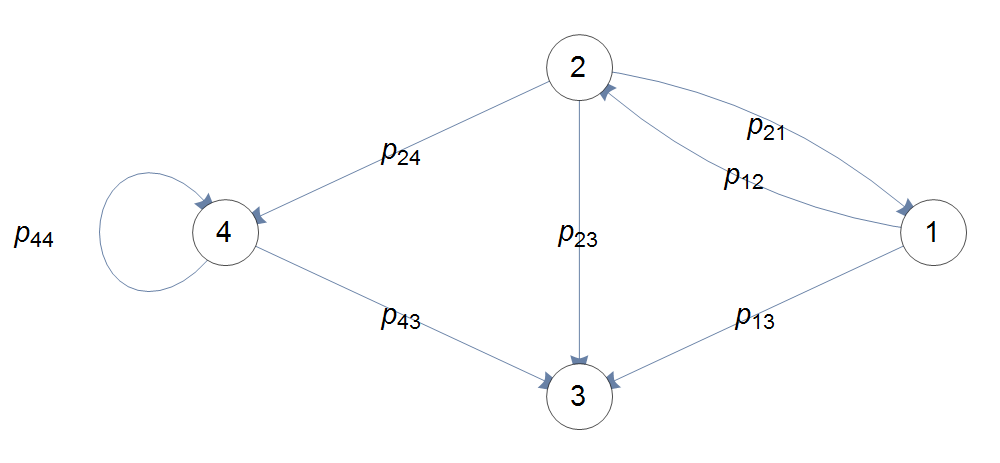
\includegraphics[width=0.7\linewidth]{graf}
\end{center}
\begin{defi}
Niech $ \left(X_n\right)_{n\ge0} $ będzie łańcuchem Markowa. Mówimy, że stan $ j\in S $ jest osiągalny ze stanu $ i\in S $, jeżeli istnieje $ n\ge0 $, że $ P\left(X_n=j|X_0=i\right)>0 $.
\end{defi}
\begin{itemize}
\item $ p_{i,j}^{(n)}>0 $
\item $ p_{i,j}^{[0,n]}>0 $
\end{itemize}
$ p_{i,j}^{[0,n]}>0 $ dla niejednorodnego łańcucha markowa nie Będzie przedmiotem rozważań.\\
Piszemy wtedy $ i\longrightarrow j $ dokładniej $ i\xrightarrow{\text{"n"}}j $
\begin{gather*}
\equiv P\left(X_0=i,X_1=i_1,\dots,X_{n-1}=i_{n-1},X_n=j\right)>0
\end{gather*}
dla pewnej ścieżki $ \left[i,i_1,i_2,\dots,i_{n-1},j\right] $
\begin{defi}
Mówimy, że stan $ i,j<in S $ komunikują się, gdy $ i\longrightarrow j $ oraz $ j\longrightarrow i $
\begin{gather*}
\left[
p_{ij}^{(n)}>0\wedge
p_{ji}^{(m)}>0
\right]
\end{gather*}
Piszemy wtedy
\begin{gather*}
i\longleftrightarrow j
\end{gather*}
\end{defi}
\begin{twr}
Relacja komunikowania się $ \longleftrightarrow $ jest relacją równoważności.
\begin{proof}
\begin{enumerate}
\item Zwrotność $ i\longleftrightarrow i $
\begin{gather*}
p_{ii}^{(0)}=1>0
\end{gather*}
\item Symetria $ i\longleftrightarrow j\stackrel{df}{\Leftrightarrow}i\longrightarrow j\wedge j\longrightarrow i $
\item Przechodniość $ i\longleftrightarrow j \wedge j\longleftrightarrow k\Rightarrow i\longleftrightarrow k$\\
$ i\longleftrightarrow k $?\\
$ i\longrightarrow j\wedge j\longrightarrow k $\\
$ p_{ij}^{(n)}>0 \wedge p_{jk}^{(m)}>0 $
\begin{gather*}
p_{ik}^{(n=k)}\stackrel{GK}{=}\sum_{l\in S}p_{il}^{(n)}p_{lk}^{(m)}\ge p_{ij}^{(n)}p_{jk}^{(m)}
\end{gather*}
Zatem $ i\longrightarrow k $. Analogicznie $ k\longrightarrow i $.
\end{enumerate}
\end{proof}
\end{twr}
\textbf{Wniosek.}\\
przestrzeń stanów $ S=\dot \bigcup[i]_{/\leftrightarrow},\,[i]_{/\leftrightarrow}= \left\{j\in S:i\longleftrightarrow j\right\}$
\begin{gather*}
S_{/\leftrightarrow}\quad \text{przestrzeń ilorazowa}
\end{gather*}
Przestrzeń stanów dzieli się na rozłączne klasy. Niektóre klasy są jednoelementowe. Czasami $ [i]_{\leftrightarrow}=\left\{i\right\} $
\begin{defi}
Dla ustalonego łańcucha Markowa $ \left(X_n\right)_{n\ge 0} $ o macierzy prawdopodobieństw przejść $ P=\left[p_{ij}\right] $ okresem stanu $ i $ nazywamy liczbę
\begin{gather*}
d(i)=NWD\left\{n\ge0:p_{ij}^{(n)}>0\right\}=
NWD\left\{n-m:pp_{ij}^{(n)},P_{ij}^{(m)}>0\right\}
\end{gather*}
\end{defi}
\textbf{Uwaga!}\\
Jeżeli $ \forall_{n\ge 1}\;p_{ii}^{(n)}=0 $, to $ d(i)=\infty  $.\\
Jeżeli $ d(i)=1 $, to stan $ i $ nazywamy aperiodycznym.
\begin{prz}
\begin{gather*}
P\left(X_{n+1}=j|X_n=i\right)=\left \{
\begin{array}{lll}
	p & j=i+1            &  \\
	q & j=i-1            &  \\
	0 & \text{pozostałe} &
\end{array}
\right .
\end{gather*}
$ P_{ii}^{(2n)}>0\\
p_{ii}^{(2n+1)}\equiv0 $\\
Konkluzja
\begin{gather*}
\forall_{i\in \mathbb Z}\;d(i)=d=2.
\end{gather*}
$ i\longleftrightarrow j $ dla dowolnych $ i,j\in \mathbb Z $
\end{prz}
\begin{defi}
Niech $ \left(X_n\right)_{n\ge 0} $ będzie jednorodnym łańcuchem Markowa. Mówimy, że łańcuch Markowa jest nieprzewiedlny (\emph{irreducible}), jeśli
\begin{gather*}
\forall_{i,j\in S}\;i\longleftrightarrow j.
\end{gather*}
\end{defi}
\chapter{7 grudnia 2015}
\begin{defi}
Niech $ \left(X_n\right)_{n\ge 0} $ będzie łańcuchem Markowa (z czasem dyskretnym i skończoną lub przeliczalną przestrzenią stanów $ S $). Mówimy, że łańcuch $ X\left(_n\right)_{n\ge 0} $ jest nieprzewiedlny, gdy
\begin{gather*}
\forall_{i,j\in S}\;i\longleftrightarrow j.
\end{gather*}
\end{defi}
\begin{twr}
Niech $ \left(X_n\right)_{n\ge0} $ będzie jednorodnym łańcuchem Markowa(z czasem dyskretnym i skończoną lub przeliczalną przestrzenią stanów $ S $) o macierzy prawdopodobieństw przejść $ \left[p_{ij}\right]_{S\times S} $. Jeżeli $ i\longleftrightarrow j $, to $ d(i)=d(j) $.\\
Przypomnienie: $ d(i)=NWD\left\{n\ge0:p_{ii}^{(n)}>0\right\} $
\end{twr}
\begin{proof}
$ i\longleftrightarrow j,P_{ij}^{(n)}>0,p_{ji}^{(m)}>0 $ dla pewnych $ n.m $ (myślimy, że $ i\neq j $)
\begin{gather*}
p_{ii}^{(n+m)}=\sum_{k\in S}p_{ik}^{(n)}p_{kj}^{(m)}\ge p_{ij}^{(m)}>0
\end{gather*}
$ p_{ii}^{l(n+m)}>0 $
\begin{gather*}
\underbrace{p_{ii}^{(n+m)}\cdot p_{ii}^{(n+m)}\dots p_{ii}^{(n+m)}}_{l\text{ razy}}
\end{gather*}
$ d(j)=p_{jj}^{(s)}>0 $
\begin{gather*}
p_{ii}^{(n+s+m)}\ge p_{ij}^{(n)}p_{jj}^{(s)}p_{ji}^{(m)}
\end{gather*}
$ p_{ii}^{(n+m)}>0 \\
d(i)|n+s+m=n+m+s\\
d9i)|n+m$\\
Stąd $ d(i)|s $ każde takie $ s $, ze $ p_{jj}^{(s)}>0 $.\\
Z teorii podzielności liczb naturalnych $ d(i)|d(j) $.\\
Z symetrii $ \longleftrightarrow\; d(j)|d(i) $.\\
Ostatecznie $ d(i)=d(j) $
\end{proof}
\textbf{Winosek}\\
Jeżeli łańcuch Markowa jest nieprzewiedlny, to
\begin{gather*}
\forall_{i,j\in S}\; d(i)=d(j)
\end{gather*}
Oznaczenia:\\
$ \left(X_n\right)_{n\ge0} $ - łańcuch Markowa jednorodny o macierzy prawdopodobieństw przejść $ P=\left[p_{ij}\right] _{S\times S}$
\begin{align*}
&f_{ij}^{(n)}=P\left(X_1\neq j,\dots,X_{n-1}\neq j,X_n=j\right),\quad n\ge 1\\
&f_{ij}=\sum_{n=1}^{\infty }f_{ij}^{(n)}=
\sum_{n=1}^{\infty }P\left(X_1\neq j,\dots,X_{n-1}\neq j,X_n=j\right)
=\\=
&P\left(\bigcup_{n=1}^{\infty }\left\{X_1\neq j,\dots,X_{n-1}\neq j,X_n=j\right\}\right)
=\\=
&P\left(\exists_{n\ge 1}\;X_n=j|X_0=i\right)
\end{align*}
Moment Markowa
\begin{gather*}
T_{ij}\stackrel{df}{=}\inf\left\{n\ge1:X_n=j,X_0=i \right\}
\end{gather*}
Pierwsza chwila uderzenia w stan $ j $.
\begin{gather*}
T_j\stackrel{df}{=}\inf\left\{n\ge1:X_n=j\right\}
\end{gather*}
Ogólnie
\begin{align*}
&T_D\stackrel{df}{=}\inf \left\{n\ge1:X_n\in D\right\},D\subseteq S\qquad\text{hitting time}\\
&P\left(T_{ij}<\infty |X_0=i\right)=P_i\left(T_{ij}<\infty \right)=f_{ij}
\end{align*}
\begin{defi}
Niech $ \left(X_n\right)_{n\ge 1} $ będzie łańcuchem Markowa z macierzą prawdopodobieństw przejść $ P\left[p_{ij}\right]_{S\times S} $. Mówimy, że stan $ j\in S $ jest powracający, jeżeli $ f_{jj}=1 $.\\
Mówimy, że stan $ j\in S $ jest chwilowy, jeżeli $ f_{jj}<1 $.
\end{defi}
\begin{twr}[Charakteryzacja stanów powracających]Neich $ \left(X_n\right)_{n\ge0} $ będzie jednorodnym łańcuchem markowa z macierzą prawdopodobieństw przejść $ P=\left[p_{ij}\right] _{S\times S}$. Wówczas następujące warunki są równoważne:
\begin{enumerate}
\item stan $ j $ jest powracający
\item $ P\left(\left\{\omega\in\Omega:X_n(\omega)=j\text{ dla nieskończenie wielu }n\in \mathbb N \right\}|X_0=j\right)=1 $
\item $ \sum_{n=1}^{}p_{jj}^{(n)}=\infty $
\end{enumerate}
\end{twr}
\begin{align*}
&L(\omega)=\#\left\{n\ge 1:X_n=j\right\}=\sum_{n=1}^{\infty }\mathbbm1_{\left\{j\right\}}\left(X_n(\omega)\right)\\
&\left\{L_j\ge1\right\}=\left\{T_j(\omega)<\infty \right\}\\
&\left\{L_j\ge 2\right\}=\left\{\exists_{n\ge 1}\;X_{t_j+n}=j\right\}\\
&T_j^{[2]}(\omega)=\inf\left\{n>T_j(\omega):X_n(\omega)=j\right\}&&\text{chwila drugiego trafienia w }j\\
&T_j^{[k]}(\omega)=\inf\left\{n>T_j^{[k-1]}(\omega):X_n(\omega)=j\right\}&&\text{chwila $ k $-tego trafienia do }j
\end{align*}
$ f_{jj}=
P\left(T_j<\infty \right)=
P\left(L_j\ge1\right)\\
P\left(L_j\ge2\right)=P\left(\exists_{n\ge 1}\;X_{t_j^{[1]}=j|X_0=j}\right) $
\begin{align*}
T_j^{[1]}=&\sum_{l=1}^{\infty }P\left(\exists_{n\ge 1}\;X_{T_j^{[1]}+n}(\omega)=j|T_j^{[1]}=l\right)P\left(T_j^{[1]}=l|X_0=j\right)
=\\=&
\sum_{l=1}^{\infty }f_{jj}\cdot P\left(T_j^{[1]}=l|X_0=j\right)
=\\=&
f_{jj}\cdot\sum_{l=1}^{\infty } P\left(T_j^{[1]}=l|X_0=j\right)
=\\=&
f_{jj}\cdot P\left(T_j^{[1]}<\infty |X_0=j\right)
=
f_{jj}^2
\end{align*}
W ten sam sposób
\begin{gather*}
P\left(L_j\ge m\right)=f_{jj}^m
\end{gather*}
\begin{proof}
$ (1)\Rightarrow(2) $\\
Jeżeli $ f_{jj}=1 $, to
\begin{align*}
&\forall_{n\in \mathbb N }\;P\left(L_j\ge m\right)=f_{jj}^{m}=1^m=1\\
&P\left(\left\{\omega\in\Omega:L_j(\omega)=\infty \right\}\right)=P\left(\bigcap_{n=1}{\infty }\left\{L_j\ge m\right\}\right)=\lim\limits_{m\to\infty} P\left(L_j\ge m\right)=1\\
&P\left(\left\{\omega\in\Omega:\sum_{n=1}^{\infty }\mathbbm1_{\left\{j\right\}}\left(X_n(\omega)=\infty )\right)\right\}\right)=P\left(\left\{\omega\in\Omega:L_j(\omega)=\infty \right\}\right)=1
\end{align*}
$ (2)\Rightarrow(3) $
\begin{align*}
&\sum_{n=1}^{\infty }p_{jj}^{(n)}
=\\=&
\sum_{n=1}^{\infty }\int\limits_{\Omega}\mathbbm1_{\left\{j\right\}}\left(X_n\right)\,dP_j
=\\=&
\sum_{n=1}^{\infty }\mathbb E _j\mathbbm1_{\left\{j\right\}}\left(X_n\right)
=\\=&
\mathbb E _j\sum_{n=1}^{\infty }\mathbbm1_{\left\{j\right\}}\left(X_n\right)
=\\=&
\mathbb E _jL_j(\omega)=\infty 
\end{align*}
$ (3)\Rightarrow(1) $\\
Przypuśćmy, że $ f_{jj}<1  $.\\
$ P_j\left(L_j\ge m\right)=f_{jj}^m $
\begin{gather*}
\sum_{n=1}^{\infty }P_j\left(L_j\ge m\right)=\sum_{n=1}^{\infty }f_{jj}^m=\frac{f_{jj}}{1-f_{jj}}<\infty \\
\mathbb E _{P_j}\left(L_j\right)=\sum_{n=1}^{\infty }p_{jj}^{(n)}=\infty 
\end{gather*}
Sprzeczność.
\end{proof}
\begin{lem}
$ \left(X_n\right)_{n\ge 0} $ jednorodny łańcuch Markowa z macierzą prawdopodobieństw przejść $ P=\left[p_{ij}\right] _{S\times S}$. Jeżeli $ j $ jest stanem powracającym oraz $ j\longleftrightarrow i (f_{ji}>0)$. Wówczas $ f_{ij}=1 $.
\end{lem}
\begin{proof}$  $\\
$ j \longrightarrow i \Rightarrow \exists_{n_0}\;p_{ji}^{(n_0)}>0$\\
$ P\left(L_j=\infty |X_0=j\right)=1 $. Zatem istnieje $ n>n_0 $ takie, że $ X_n=j $.\\
$ P\left(\left\{\omega\in\Omega:X_n(\omega)=j\text{ dla pewnego }n>n_0|X_0=j\right\}\right)=1 $
\begin{align*}
1=&P_j\left(\exists_{n>n_0}\;X_n=j\right)
=\\=&
\sum_{l\in S}P\left(\exists_{n>n_0}\;X_n=j|X_{n_0}=l\right)P_j\left(X_{n_0}=l\right)
=\\=&
\sum_{l\in S}P_j\left(\exists_{n\ge 1}\;X_{n+n_0}=j|X_{n_0}=l\right)p_{jl}^{(n_0)}
=\\=&
\sum_{l\in S}f_{ij}p_{jl}^{(n_0)}
\end{align*}
\begin{align*}
&1-\sum_{l\in S}f_{ij}p_{jl}^{(n_0)}
=\\=&
\sum_{l\in S}p_{jl}^{(n_0)}-\sum_{l\in S}f_{ij}p_{jl}^{(n_0)}
=\\=&
\sum_{l\in S}\underbrace{p_{jl}^{(n_0)}}_{\ge 0}(\underbrace{1-f_{lj}}_{\ge 0})
\end{align*}
Jeżeli $ p_{jl}^{(n_0)}>0 $, to $ 1-f_{lj}=0 $\\
Właśnie $ j\longrightarrow i $ spełnia $ p_{ji}^{(n_0)}>0 $ zatem ostatecznie $ f_{ij}=1 $
\end{proof}
\begin{lem}
Niech $ \left(X_n\right)_{n\ge 0} $ będzie jednorodnym łańcuchem Markowa o macierzy prawdopodobieństw przejść $ P=\left[p_{ij}\right] $. Jeżeli $ j\in S $ jest stanem chwilowym to dla dowolnego $ i\in S $
\begin{gather*}
\sum_{n=1}^{\infty }p_{ij}^{(n)}<\infty 
\end{gather*}
co implikuje
\begin{gather*}
\lim\limits_{n\to\infty} p_{ij}^{(n)}=0
\end{gather*}
\end{lem}
\begin{proof}
Ustalmy $ i\in S $. Jeżeli $ \forall_{n\ge 1}\;p_{ij}^{(n)}=0 $ (tzn. $ \neg\left(i\longleftrightarrow j\right) $), to oczywiście
\begin{gather*}
\sum_{n=1}^{\infty }p_{ij}^{(n)}=\sum_{n=1}^{\infty }0=0
\end{gather*}
Zatem będziemy rozpatrywali przypadek $ \exists_{n\ge 1}\;p_{ij}^{(n)}>0 $.
\begin{align*}
p_{ij}^{(n)}
=&
P\left(X_n=j|X_0=i\right)
=\\=&
\frac{P\left(X_n=j,X_0=i\right)}{P\left(X_0=i\right)}
=\\=&
\frac{P\left(\left\{X_n=j\right\}\cap\left\{T_j\le n\right\}\cap \left\{X_0=i\right\}\right)}{P\left(X_0=i\right)}
=\\=&
\frac{P\left(\left\{X_n=j\right\}\cap\bigcup\limits_{k=1}^\infty \left\{T_j=k\right\}\cap \left\{X_0=i\right\}\right)}{P\left(X_0=i\right)}
=\\=&
\sum_{k=1}^{n }\frac{P\left(\left\{X_n=j\right\}\cap \left\{X_1\neq j,\dots,X_{k-1}\neq j,X_k=j\right\}\cap \left\{X_0=i\right\}\right)}{P\left(X_0=i\right)}
=\\=&
\sum_{k=1}^{n}\frac{P\left(X_n=j|X_k=j,X_{k-1}\neq j,\dots,X_0=i\right)}{P\left(X_0=i\right)}P\left(X_k=j,X_{k-1}\neq j,\dots,X_0=i\right)
=\\=&
\sum_{k=1}^{n}p_{jj}^{(n-k)}f_{ij}^{[k]}=p_{ij}^{(n)}
\end{align*}
W ostatnim przejściu pamiętamy, że $ \sum_{n=0}^{\infty }p_{jj}^{(n)}<\infty  $

\begin{align*}
\sum_{n=1}^{\infty }p_{dół}^{(n)}
=&
\sum_{n=1}^{\infty }\left(\sum_{k=1}^{n}f_{ij}^{[k]}p_{jj}^{(n-k)}\right)
=\\=&
\sum_{k=1}^{\infty }f_{ij}^{[k]}\sum_{n=k}^{n}p_{jj}^{(n-k)}
=\\=&
\left(\sum_{n=1}^{n}p_{jj}^{(n)}\right)\sum_{k=1}^{\infty }f_{ij}^{[k]}<\infty 
\end{align*}
\begin{gather*}
\sum_{n=1}^{\infty }p_{ij}^{(n)}<\infty 
\end{gather*}
\end{proof}
\textbf{Wniosek}\\
Jeżeli przestrzeń stanów $ S $ dla jednorodnego łańcucha Markowa $ \left(X_n\right)_{n\ge 0} $ jest skończona ($ \#S<\infty  $), to istnieje co najmniej jedne stan powracający.
\begin{proof}
Przypuśćmy, że wszystkie stany są chwilowe.
\begin{gather*}
\forall_{i\in S}\forall_{j\in S}\;\sum_{n=0}^{\infty }p_{dół}^{(n)}=\rho_{ij}<\infty 
\end{gather*}
\begin{gather*}
\sum_{j\in S}\sum_{i\in S}\sum_{n=0}^{\infty }p_{dół}^{(n)}=\sum_{i,j\in S}\rho_{ij}<\infty \\
\sum_{n=0}^{\infty }\sum_{i\in S}\sum_{j\in S}p_{dół}^{(n)}=\sum_{n=0}^{\infty }\left(\#S\cdot 1\right)=\infty 
\end{gather*}
\end{proof}
\textbf{Uwaga!}\\
Może się zdarzyć, że dla $ \#S=\infty  $ nie ma w ogóle stanów powracających.

Oznaczenia\\
Część konserwatywna procesu $ \left(X_n\right)_{n\ge 0} $
\begin{gather*}
C=\left\{j\in S:j\text{ jest stanem powracającym}\right\}=\left\{j\in S:\sum_{n=1}^{\infty }p_{jj}^{(n)}=\infty \right\}
\end{gather*}
Część dysypatywna procesu $ \left(X_n\right)_{n\ge 0} $
\begin{gather*}
D=\left\{j\in S:p_{jj}^{(n)}\infty \right\}
\end{gather*}
\begin{defi}
Niech $ \left(X_n\right)_{n\ge 0} $ będzie jednorodnym łańcuchem Markowa na przestrzeni stanów $ S $ o macierzy prawdopodobieństw przejść $ P=\left[p_{ij}\right] _{S\times S}$. Mówimy, że $ A\subseteq S $ jest zamknięty (niezmienniczy), jeśli spełnia
\begin{gather*}
\forall_{i\in A}\forall_{j\notin A}\;p_{ij}=0
\end{gather*}
Inaczej
\begin{gather*}
P\mathbbm1_{A}(i)=\sum_{j\in A}p_{ij}=\sum_{j\in A}\mathbbm1_{A}(j)p_{ij}
\end{gather*}
\end{defi}
\begin{twr}
Część konserwatywna procesu jest zbiorem zamkniętym.
\begin{proof}
Niech $ i\in C $ oraz $ i\longleftrightarrow j $. Przypuśćmy $ p_{ij}^{(n_0)}>0 $. Wtedy $ f_{ij}=1 $ z lematu.\begin{gather*}
\exists_{n_0\ge 1}\;p_{ij}^{(n_0)}>0
\end{gather*}
\begin{align*}
\sum_{k=1}^{\infty }p_{jj}^{(k)}
\ge\\\ge&
\sum_{k=m_0+n_0+1}^\infty p_{jj}^{(k)}
\ge\\\ge&
\sum_{k=m_0+n_0+1}^\infty p_{ji}^{(m_0)}p_{ii}^{(k-n_0-m_0)}p_{ij}^{(n_0)}
=\\=&
\underbrace{p_{ji}^{(m_0)}}_{\ge 0}
\sum_{l=1}^\infty
\underbrace{p_{ii}^{(l)}}_{\infty }
\underbrace{p_{ij}^{(n_0)}}_{\ge 0}
=\infty 
\end{align*}
\end{proof}
\end{twr}
\chapter{14 grudnia 2015}
Komentarz związany z kolokwium\\
$ \left\{N(t)\right\}_{t\ge 0} $ jednorodny proces Poissona z intensywnością $ \lambda>0 $\\
$ cov\left(N(t),N(s)\right)=\lambda\left(t\wedge s\right)=\lambda\cdot\min\left\{s,t\right\} $\\
$ \mathbb E \left(N(t)\cdot N(s)\right)=cov\left(N(t),N(s)\right)+\mathbb E N(t)\mathbb E N(s)=\lambda\cdot\min\left\{s,t\right\}+\lambda s\cdot\lambda t $
dla $ t \ge s $\\
$ \mathbb E \left(N(t)\cdot N(s)\right)=\mathbb E \left(\left(N(t)\cdot N(s)\right)\cdot N(s)+N(t)^2\right) $
koniec komentarza

Niech $ \left(X_n\right)_{n\ge 0} $ będzie jednorodnym łańcuchem markowa z macierzą prawdopodobieństw przejść $ P=[p_{ij}] $. Oznaczmy
\begin{gather*}
\tau_j=\left \{
\begin{array}{l}
	\min\left\{n\ge 1:X_n(\omega)=j\right\}                     \\
	\infty , \text{ jeżeli }\forall_{n\ge 1}\; X_n(\omega)\neq j
\end{array}
\right .
\end{gather*}
moment Markowa.
\begin{gather*}
m_{jj}=\mathbb E _j\left(\tau_j\right)=\sum_{n=1}^{\infty }n\cdot f_{jj}^{[n]}=\int\limits_{\Omega}\tau_j\,dP\left(\cdot|X_0=j\right)
\end{gather*}
Przypomnienie
\begin{gather*}
f_{jj}^{[n]}=P\left(X_1\neq j,\dots,X_{n-1}\neq j,X_n=j|X_0=j\right)
\end{gather*}
\begin{defi}
Mówimy, że stan $ j\in C $ jest dodatnio powracający, jeżeli $ m_{jj}<\infty  $.\\
Mówimy, że stan $ j\in C $ jest 0 powracający, jeżeli $ m_{jj}=\infty  $.
\end{defi}
\textbf{Uwawga!}\\
Oczywiście, jeżeli $ j\in D=S\backslash C $ to $ P_j\left(\tau_j=\infty \right)>0 $. Zatem
\begin{gather*}
\forall_{j\in D}\;m_{jj}=\infty 
\end{gather*}
\begin{defi}
Mówimy, że miara probabilistyczna $ \mu  $na $ (S, 2^S) $ jest niezmiennicza (stacjonarna) dla $ j $ łańcucha Markowa $ \left(X_n\right)_{n\ge 0} $ o macierzy prawdopodobieństw przejść $ P $, jeżeli
\begin{gather*}
\forall_{j\in S}\;\sum_{i\in S}\mu_i\cdot p_{ij}=\mu_j\\
\underline{\mu}\circ P=\underline{\mu}
\end{gather*}
\end{defi}
\begin{gather*}
\mathcal P\left(S\right)\ni\underline{\mu}\to\underline{\mu}\circ P\in \mathcal P\left(S\right)\\
\left(\mu_0,\mu_1,\mu_2,\dots \right)\circ
\begin{bmatrix}
	p_{0,0} & p_{0,1} & \ldots \\
	p_{1,0} & p_{1,1} & \ldots \\
	\vdots  & \vdots  & \ddots
\end{bmatrix}=
\left(\mu_0,\mu_1,\mu_2,\dots \right)
\end{gather*}
\textbf{Uwaga!}\\
Niech $ X_0 $ ma rozkład $ \underline{\mu}\left[P\left(X_0=i\right)=\mu_i\right] $. Rozkład $ x_1 $?
\begin{gather*}
P\left(X_1=j\right)=
\sum_{j\in S}P\left(X_1=j|X_0=i\right)P\left(X_0=i\right)=
\sum_{i\in S}\mu_i\cdot p_{ij}=\underline{\mu}\circ P
\end{gather*}
\begin{align*}
\underline{\mu}&\text{ rozkład }X_0\\
\underline{\mu}\circ P&\text{ rozkład }X_1\\
\underline{\mu}\circ P^2&\text{ rozkład }X_2\\
\end{align*}
\begin{twr}
Niech $ \left(X_n\right)_{n\ge 0} $ będzie jednorodnym łańcuchem Markowa o macierzy prawdopodobieństw przejść $ P=\left[p_{ij}\right] _{S\times S}$. Jeżeli $ r\in C $ jest stanem dodatnio powracającym, wówczas istnieje dokładnie jedna miara probabilistyczna niezmiennicza $ \pi$ o własności $ \pi_r>0 $. Co więcej
\begin{gather*}
\pi_r=
\left \{
\begin{array}{ll}
\frac{1}{m_{rr}=\frac{1}{\mathbb E _r\tau_r}},&j=r\\
0,&j\notin [r]\\
\frac{1}{\mathbb E _r\tau_r}\cdot \left(1+P_{r_j}+\sum_{n=1}^{\infty }\sum_{i_1,\dots,i_n\in S\backslash\{r\}}
p_{ri_1}\cdot p_{i_1i_2}\cdot\dots p_{i_{n-1}j}\right),&j\in [r]\wedge j\neq r
\end{array}
\right .
\end{gather*}
\end{twr}
\textbf{Wniosek}
\begin{gather*}
C=C_+\cup C_0\\
C_+=\left\{r\in C:\mathbb E _r\tau_r<\infty \right\}=\left\{j\in C:\mu_j>0\text{ dla pewnej }\underline{\mu}\circ P=\underline{\mu}\right\}
\end{gather*}
\begin{twr}
Niech $ \left(X_n\right)_{n\ge 0} $ będzie jednorodnym łańcuchem Markowa na przestrzeni stanów $ S $ o macierzy prawdopodobieństw przejść $ P[p_{ij}] $. Łańcuch $ \left(X_n\right)_{n\ge 0} $jest stacjonarny wtedy i tylko wtedy, gdy $ \mu^{(0)}=\mathcal L\left(X_0\right) $ rozkład początkowy jest miarą niezmienniczą.
\end{twr}
\begin{proof}$ \Rightarrow $
Ze stacjonarności $ \left(X_0,X_1,\dots,X_n\right)\sim \left(X_1,X_2,\dots,X_{n+1}\right)$. $ \mathcal L(X_0)=\mathcal L(X_1) $. Ale pamiętamy, że $ \underline{\mu}^{(1)}=\underline{\mu}^{(0)}\circ P $, czyli mamy $ \underline{\mu}^{(0)}=\mu^{(0)}\circ P $.
\textbf{Uwaga!}\\
Iterując $ \underline{\mu}^{(n)}=\underline{\mu}^{(0)}\circ P^n $ dla dowolnego $ n\ge 0 $\\
$ \Leftarrow $\\
Załóżmy, że $ \underline{\mu}^{(0)}=\underline{\mu}^{(0)}\circ P $.\\
$ \mu_{(X_0,\dots,X_n)}=\mu_{(X_k,\dots,X_{n+k})} $ dla dowolnego $ k=1,2,\dots $?
\begin{gather*}
P\left(X_0=i_0,X_1=i_1,\dots,X_n=i_n\right)=
P\left(X_k=i_0,X_{k+1}=i_1,\dots,X_{k+n}=i_n\right)
\end{gather*}
dla dowolnego wyboru $ i_0,i_1,\dots,i_n\in S $
\begin{align*}
&P\left(X_0=i_0\right)p_{i_0i_1}\cdot p_{i_1i_2}\cdot\ldots \cdot p_{i_{n-1}i_n}\\
&P\left(X_k=i_0\right)p_{i_0i_1}\cdot p_{i_1i_2}\cdot\ldots \cdot p_{i_{n-1}i_n}\\
&P\left(X_k=i_0\right)=\left(\underline{\mu}^{(0)}\circ P^k\right)_{i_0}=\mu_{i_0}^{(0)}=P\left(X_0=i_0\right)
\end{align*}
Stąd $ P\left(X_0=i_0\right)p_{i_0i_1}\cdot p_{i_1i_2}\cdot\ldots \cdot p_{i_{n-1}i_n}=P\left(X_k=i_0\right)p_{i_0i_1}\cdot p_{i_1i_2}\cdot\ldots \cdot p_{i_{n-1}i_n} $ dla dowolnego $ k\ge 0 $. Czyli otrzymaliśmy stacjonarność $ X_0,X_1,\dots  $
\end{proof}
\begin{twr}
Niech $ \left(X_n\right)_{n\ge 0} $ będzie jednorodnym łańcuchem Markowa z macierzą prawdopodobieństw przejść $ P=[p_{ij}] $. Wówczas
\begin{enumerate}
\item
\begin{gather*}
\lim\limits_{n\to\infty} \frac{1}{n}\sum_{k=1}^{n}p_{jj}^{(k)}=\frac{1}{m_{jj}}
\end{gather*}
\item 
\begin{gather*}
\lim\limits_{n\to\infty} p_{jj}^{(n)}=\frac{1}{m_{jj}}
\end{gather*}
jeśli dodatkowo założymy, że $ j $ jest aperiodyczny
\item 
\begin{gather*}
\lim\limits_{n\to\infty} p_{jj}^{(n)}=\frac{d}{m_{jj}}
\end{gather*}
jeżeli dodatkowo założymy, że $ d(j)=d $.
\end{enumerate}
\end{twr}
\textbf{Uwaga!}\\
Powyższe twierdzenie nosi nazwę średniego twierdzenia ergodycznego na $ l^1 $.
\newpage
\begin{center}
{\Large\textsc{Proces ruchu Browna}}
\end{center}
Intuicyjne wprowadzenie w teorię procesów ruchu Browna (procesów Wienera).\\
$ X_1,\dots  $ ciąg niezależnych zmiennych losowych o tym samym rozkładzie takich, że 
$ P\left(X_k=-1\right)=P\left(X_k=1\right)=\frac{1}{2} $\\
$ X_t^{\substack{\Delta x\\\Delta t}} =\Delta x\cdot X_1+\Delta x\cdot X_2+\dots\Delta x\cdot X_{\left \lfloor\frac{t}{\Delta t}\right \rfloor}$ dla $ t\ge 0 $\\
Spacer losowy o skokach $ \pm\Delta x $\\
\begin{gather*}
\mathbb E X_t^{\substack{\Delta x\\\Delta t}}=\sum_{j=1}^{\left \lfloor\frac{t}{\Delta t}\right \rfloor}\mathbb E \Delta x\cdot X_1=0\\
\Var X_t^{\substack{\Delta x\\\Delta t}}=\sum_{j=1}^{\left \lfloor\frac{t}{\Delta t}\right \rfloor}\Var\left(\Delta x\cdot X_j\right)=\Delta x^2\cdot \left \lfloor\frac{t}{\Delta t}\right \rfloor\cdot 1
\end{gather*}
Dobieramy $ \Delta x,\Delta t $
\chapter{21 grudnia 2015}
$ X_t^{\substack{\Delta x\\\Delta t}} =\Delta x\cdot X_1+\dots +\Delta x\cdot X_{\left \lfloor\frac{t}{\Delta t}\right \rfloor}, X_1,X_2,\dots$ - i.i.d.\\
$ X_j\in\left\{-1,1\right\} $\\
$P\left(X_j=1\right)=P\left(X_j=-1\right)=\frac{1}{2}$
\begin{gather*}
X_t^{\substack{\Delta x\\\Delta t}}\xrightarrow[\substack{\Delta x\to 0^+\\\Delta t\to 0^+}]{?}
\end{gather*}
Załóżmy, że $ \Delta x=c\sqrt{\Delta t} $\\
$ c>0 $ - stała
\begin{gather*}
\frac{\Delta x\cdot X_1+\dots +\Delta x\cdot X_{\left \lfloor\frac{t}{\Delta t}\right \rfloor}}{\sqrt{\left \lfloor\frac{t}{\Delta t}\right \rfloor}\Delta x} \stackrel{\mathcal D}{\Longrightarrow}\mathfrak X\sim \mathcal N(0,1)\\
\Delta x\cdot X_1+\dots +\Delta x\cdot X_{\left \lfloor\frac{t}{\Delta t}\right \rfloor}
=\\=
\sqrt{\left \lfloor\frac{t}{\Delta t}\right \rfloor\Delta x^2}\cdot
\frac{\Delta x\cdot X_1+\dots +\Delta x\cdot X_{\left \lfloor\frac{t}{\Delta t}\right \rfloor}}{\sqrt{\left \lfloor\frac{t}{\Delta t}\right \rfloor}\Delta x}\stackrel{\mathcal D}{\Longrightarrow}\mathcal N(0,c^2t)\\
\left(\frac{t}{\Delta t}-1\right)\Delta x^2\le \left \lfloor\frac{t}{\Delta t}\right \rfloor\Delta x^2\le \frac{t \Delta x^2}{\Delta t}
\end{gather*}
\begin{defi}
Dla $ t\ge 0 $ niech
\begin{gather*}
X_t\stackrel{df}{=}\lim\limits_{\substack{\Delta t\to 0\\\Delta x=c\sqrt{\Delta t}}} X_t^{\substack{\Delta x\\\Delta t}}
\end{gather*}
\end{defi}

\textbf{Wniosek}\\
$ X_t\sim\mathcal N(\mu=0,\Var=c^2t) $
\begin{gather*}
\underbrace{\Delta xX_1+\dots+\Delta xX_{\left \lfloor\frac{s}{\Delta t}\right \rfloor}}_{X_s}+
\underbrace{\Delta xX_{\left \lfloor\frac{s}{\Delta t}\right \rfloor+1}+\dots+\Delta xX_{\left \lfloor\frac{t}{\Delta t}\right \rfloor}}_{X_{t-s}}\to X_t
\end{gather*}
\begin{align*}
X_s\sim \mathcal N(0,c^2s)&&
X_{t-s}\sim \mathcal N(0,c^2(t-s))
\end{align*}
$ X_t-X_s $ ten sam rozkład co $ X_{t-s} $ oraz $ X_{t-s}\Perp X_s $

Otrzymany proces jest procesem o przyrostach niezależnych, jednorodnych. Mała kolizja oznaczeń; proces graniczny oznaczamy $ \left\{X_t\right\}_{t\ge 0} $ i wyjściowy ciąg Bernoulliego niestety oznaczamy $ X_1,X_2,\dots  $.
\begin{defi}
Mówimy, że proces stochastyczny $ \mathfrak X=\left\{X_t\right\} _{t\ge 0}$ jest procesem ruchu Browna, jeżeli spełnia
\begin{enumerate}
\item $ X_0=0 $ z pr. 1
\item $ \left\{X_t\right\}_{t\ge 0} $ jest procesem o przyrostach niezależnych i jednorodnych
\item $ \forall_{t\ge0}\;X_t\sim \mathcal N(0,c^2t) $
\item Trajektorie $ X_t(\omega) $ są funkcjami ciągłymi (zmiennej $ t $) dla $ P $ prawie wszystkich $ \omega\in \Omega $
\end{enumerate}
\end{defi}
Pytanie\\
Czy taki proces stochastyczny istnieje?\\
Heurystycznie pokazaliśmy, że atk.\\
Tak, istnieje (dowód pełny podał Wiener; w latach 60 piękny dowód istnienia podał Z. Ciesielski (Sopot, IMPAN))

\textbf{Uwaga!}\\
(10,(2),(3) implikuje (4) [z dokładnością do wersji]\\
Od tej pory będziemy zakładali $ c=1 $.\\
Standardowy proces ruchu Browna ma rozkłady $ X_t\sim \frac{1}{\sqrt{2\pi t}}e^{-\frac{x^2}{2t}} $. $ \Var X_t=t $
\begin{defi}
Mówimy, że proces stochastyczny $ \left\{Y_t\right\} _{t\ge 0}$ określony na $ (\Omega,\mathcal F,P) $ i wartościach w przestrzeni fazowej (stanów) $ (S<\mathcal G) $ jest procesem Markowa, jeżeli
\begin{gather*}
\forall_{n\in \mathbb N }\forall_{Y_{n-1},Y_{n-2},\dots,Y_0\in S}\forall_{B\in\mathcal G}\forall_{t_n>t_{n-1}>\dots>t_0}
\end{gather*}
zachodzi warunek Markowa
\begin{gather*}
P\left(Y_{t_n}\in B|
Y_{t_{n-1}}=y_{n-1},
Y_{t_{n-2}}=y_{n-2},
\dots,
Y_{t_{0}}=y_{0}
\right)=
P\left(Y_{t_n}\in B|
Y_{t_{n-1}}=y_{n-1}
\right)\\
F_{Y_{t_n}|
Y_{t_{n-1}}=y_{n-1},
Y_{t_{n-2}}=y_{n-2},
\dots,
Y_{t_{0}}=y_{0}}=
F_{Y_{t_n}|
Y_{t_{n-1}}=y_{n-1}}
\end{gather*}
\end{defi}
\textbf{Oznaczenie}
\begin{gather*}
P\left(Y_t\in B|Y_s=y\right)=P^{[s,t]}(y,B)\qquad 0\le s<t
\end{gather*}
funkcja prawdopodobieństwa przejścia. Czas ciągły i przestrzeń stanów (może być ciągła).
\begin{twr}
Proces ruchu Browna jest procesem Markowa.
\begin{proof}
Ustalmy $ n\in \mathbb N, \;t_0<t_1<\dots<t_{n-1}<t_n,\;y_0,y_1,\dots,y_{n-1}\in \mathbb R ,\\ B\in \mathfrak B_\mathbb R  $
\end{proof}
\begin{align*}
&P\left(X_{t_n}\in B|X_{t_{n-1}}=y_{n-1},\dots,X_{t_0}=y_0\right)
=\\=&
P\left(X_{t_n}-X_{t_{n-1}}\in B-y_{n-1}|X_{t_{n-1}}-X_{t_{n-2}}=y_{n-1}-y_{n-2},\dots,X_{t_1}-X_{t_0}=y_1-y_0,\right .\\&\left .X_{t_0}=y_0\right)
\end{align*}
Niezależność przyrostów
\begin{align*}
&P\left(X_{t_{n}}-X_{t_{n-1}}\in B-y_{n-1}\right)
=\\=&
\int\limits_{B-y_{n-1}}\frac{1}{\sqrt{2\pi(t_n-t_{n-1})}}\exp\left(-\frac{x^2}{2\left(t_n-t_{n-1}\right)}\right)\,dx
=\\=&
\int\limits_{B-y_{n-1}}\frac{1}{\sqrt{2\pi(t_n-t_{n-1})}}\exp\left(-\frac{\left(x-y_{n-1}\right)^2}{2\left(t_n-t_{n-1}\right)}\right)\,dx
=\\=&
P^{[t_{n-1},t_n]}\left(y_{n-1},B\right)
\end{align*}
\begin{gather*}
\mathbb E 
\left(\mathbbm1_{\left\{X_{t_n}\in B\right\}}|X_{t_{n-1}},\dots,X_{t_0}\right)
\stackrel{?}{=}
\mathbb E 
\left(\mathbbm1_{\left\{X_{t_n}\in B\right\}}|X_{t_{n-1}}\right)
\end{gather*}
\begin{align*}
&
P\left(X_{t_n}\in B|X_{t_{n-1}}=y_{n-1}\right)
=\\=&
P\left(X_{t_n}-y_{n-1}\in B-y_{n-1}|X_{t_{n-1}}-X_0=y_{n-1}-0\right)
=\\=&
P\left(X_{t_n}-y_{n-1}\in B-y_{n-1}|X_{t_{n-1}}-X_0=y_{n-1}\right)
\end{align*}
Niezależność przyrostów $ X_{t_n}-X_{t_{n-1}}\Perp X_{t_{n-1}}-X_0 $
\begin{align*}
&
P\left(X_{t_n}-y_{n-1}\in B-y_{n-1}\right)
=\\=&
P\left(X_{t_n-t_{n-1}}\in B-y_{n-1}\right)
=\\=&
\int\limits_{B-y_{n-1}}\frac{1}{\sqrt{2\pi(t_n-t_{n-1})}}\exp\left(-\frac{x^2}{2\left(t_n-t_{n-1}\right)}\right)\,dx
=\\=&
\int\limits_{B}\frac{1}{\sqrt{2\pi(t_n-t_{n-1})}}\exp\left(-\frac{\left(x-y_{n-1}\right)^2}{2\left(t_n-t_{n-1}\right)}\right)\,dx
\end{align*}
\end{twr}
Dygresja formalna
\begin{gather*}
\mathbb E \left(\mathbbm1_{\left\{X_{t_n}\in B\right\}}|X_{t_{n-1}},\dots,X_{t_0}\right)=P^{[t_{n-1},t_n]}\left(X_{t_{n-1},B}\right)
\end{gather*}
\begin{twr}
Jeżeli $ \left\{B_t\right\} _{t\in [0,\infty )}$ jest standardowym procesem ruchu Browna to
\begin{gather*}
\cov \left(B_s,B_t\right)=s\wedge t\;\left(=\min\left\{s,t\right\}\right)
\end{gather*}
\begin{proof}
\begin{align*}
&
\cov \left(B_s,B_t\right)
=\\=&
\mathbb E B_sB_t-\mathbb E B_s\mathbb E B_t
=\\=&
\mathbb E B_sB_t
\stackrel{s=s\wedge t}{=}\\=&
\mathbb E \left(\left(B_t-B_s+B_s\right)B_s\right)
=\\=&
\mathbb E \left(\left(B_t-B_s\right)B_s+B_s^2\right)
=\\=&
\mathbb E \left(\left(B_t-B_s\right)B_s\right)+\mathbb EB_s^2
=\\=&
\mathbb E \left(B_t-B_s\right)\mathbb E \left(B_s\right)+\Var B_s^2=s=s\wedge t
\end{align*}
\end{proof}
\end{twr}
\textbf{Ostrzeżenie}\\
Dwa różne procesy $ \left\{N_t\right\}_{t\ge 0},\left\{B_t\right\}_{t\ge 0} $ mają tę samą funkcję autokorelacji $ c(s,t)=s\wedge t $
\begin{twr}
Niech $ \left\{X_t\right\}_{t\ge0 } $ będzie standardowym procesem ruchu Browna. Dla dowolnych $ t_1<t_2<\dots<t_n,\;n\ge 1 $, wektor gaussowski $ \left(X_{t_1},X_{t_2},\dots,X_{t_n}\right) $ ma gęstość $ n $-wymiarową (niezdegenerowaną) postaci
\begin{gather*}
f_{\left(X_{t_1},X_{t_2},\dots,X_{t_n}\right)}
\left(x_1,x_2,\dots,x_n\right)=
\prod_{j=1}^{n}\int\limits_{B}\frac{1}{\sqrt{2\pi(t_j-t_{j-1})}}\exp\left(-\frac{\left(x_j-y_{j-1}\right)^2}{2\left(t_j-t_{j-1}\right)}\right)\,dx
\end{gather*}
\begin{proof}
$\left(X_{t_1}-X_{t_0},X_{t_2}-X_{t_1},\dots,X_{t_n}-X_{t_{n-1}}\right) $ ma gęstość
\begin{gather*}
f_{\left(X_{t_1},X_{t_2}-X_{t_1},\dots,X_{t_n}-X_{t_{n-1}}\right)}\left(x_1,x_2,\dots,x_n\right)
=\\=
\prod_{j=1}^{n}f_{X_{t_j-X_{t_{j-1}}}}(x_j)=
\prod_{j=1}^{n}f_{X_{t_j-X_{t_{j-1}}}}(x_j)
\frac{1}{\sqrt{2\pi(t_j-t_{j-1})}}\exp\left(-\frac{x_j^2}{2\left(t_j-t_{j-1}\right)}\right)\\
\psi\left(X_{t_1},X_{t_2}-X_{t_1},\dots,X_{t_n}-X_{t_{n-1}}\right)=
\left(X_{t_1},X_{t_2},\dots,X_{t_n}\right)
\end{gather*}
Jak wygląda $ \psi:\mathbb R^n\to \mathbb R ^n $?
\begin{align*}
&\psi \left(x_1,x_2-x_1,\dots,x_n-x_{n-1}\right)=
\left(x_1,\dots,x_n\right)\\
&\psi \left(y_1,y_2,\dots,y_n\right)=
\left(y_1,y_1+y_2,y_1+y_2+y_3,\dots,y_1+y_2+\dots+y_n\right)
\end{align*}
$ \psi $ operacja liniowa.
\begin{gather*}
f_{\psi\left(\vec Z\right)}\left(z_1,\dots,z_n\right)=f\left(\psi^{-1}\right)\left|J_{\psi^{-1}}\right|\\
\psi^{-1}\left(z_1,\dots,z_n\right)=\left(z_1,z_2-z_1,\dots,z_n-z_{n-1}\right)
\end{gather*}
Macierz
\begin{gather*}
J_{\psi^{-1}}=
\begin{bmatrix}
	1      & 0      & 0      & \ldots & 0      & 0      \\
	-1     & 1      & 0      & \ldots & 0      & 0      \\
	0      & -1     & 1      & \ldots & 0      & 0      \\
	\vdots & \vdots & \vdots & \ddots & \vdots & \vdots \\
	0      & 0      & 0      & \ldots & 1      & 0      \\
	0      & 0      & 0      & \ldots & -1     & 1
\end{bmatrix}\\
\left|J_{\psi^{-1}}\right|=1
\end{gather*}
\begin{gather*}
f_{\left(X_{t_1},X_{t_2},\dots,X_{t_n}\right)}\left(x_1,\dots,x_n\right)=
f_{\left(X_{t_1},X_{t_2}-X_{t_1},\dots,X_{t_n}-X_{t_{n-1}}\right)}\left(\psi^{-1}\left(x_1,\dots,x_n\right)\right)
=\\=
\prod_{j=1}^{n}\frac{1}{\sqrt{2\pi(t_j-t_{j-1})}}\exp\left(-\frac{\left(x_j-y_{j-1}\right)^2}{2\left(t_j-t_{j-1}\right)}\right)
\end{gather*}
\end{proof}
\end{twr}
\section{Własności trajektorii standardowego procesu ruchu Browna}
$ \mathbb R _+\ni t\to B_t(\omega) $ jest funkcją ciągłą dla $ P $ p.w. $ \omega\in\Omega $.\\
Problem różniczkowalności
\begin{gather*}
P\left(\left|\frac{X_{t+\Delta t}(\omega)-X_t(\omega)}{\Delta t}\right|>n\right)=
2\int\limits_{n}^{\infty }\frac{1}{\sqrt{2\pi \frac{1}{\Delta t}}}\exp\left(-\frac{x^2}{2\cdot \frac{1}{\Delta t}}\right)\,dx\xrightarrow[\Delta t\to0]{}1
\end{gather*}
Według prawdopodobieństwa $ \left|\frac{X_{t+\Delta t}-X_t}{\Delta t}\right|\xrightarrow[\Delta t\to0]{}\infty $\\
Trajektorie procesu ruchu Browna są nigdzie różniczkowalne z prawdopodobieństwem 1.
\begin{twr}[Prawo iterowania logarytmu]
Niech $ \left\{B_t\right\} _{t\ge 0}$ będzie standardowym procesem Wienera (ruch Browna). Wówczas
\begin{align*}
&P\left(\left\{\omega\in\Omega:\limsup_{t\to+\infty }\frac{B_t(\omega)}{\sqrt{2t\ln \left(\ln t\right)}}=1\right\}\right)=1\\
&P\left(\left\{\omega\in\Omega:\liminf_{t\to+\infty }\frac{B_t(\omega)}{\sqrt{2t\ln \left(\ln t\right)}}=-1\right\}\right)=1
\end{align*}
\end{twr}
\begin{twr}[Lokalne prawo iterowania logarytmu]
Niech $ \left\{B_t\right\} _{t\ge 0}$ będzie standardowym procesem Wienera (ruch Browna). Wówczas
\begin{align*}
&P\left(\left\{\omega\in\Omega:\limsup_{t\to0^+ }\frac{B_t(\omega)}{\sqrt{2t\ln \left(\ln t\right)}}=1\right\}\right)=1\\
&P\left(\left\{\omega\in\Omega:\liminf_{t\to0^+ }\frac{B_t(\omega)}{\sqrt{2t\ln \left(\ln t\right)}}=-1\right\}\right)=1
\end{align*}
\end{twr}

\textbf{Wniosek}\\
Z prawdopodobieństwem 1, trajektoria $ B_t(\omega) $ w okolicy $ t_0=-0 $ przecina poziom 0 nieskończenie wiele razy.

\textbf{Wniosek}\\
Z prawdopodobieństwem 1, trajektoria $ B(\omega) $
\begin{align*}
\limsup_{t\to0^+}\frac{B_t(\omega)}{t}=+\infty
&&
\liminf_{t\to0^+}\frac{B_t(\omega)}{t}=-\infty
\end{align*}
Syntezując punkty skupienia $ \frac{B_t(\omega)}{t}\underset{t\to 0^+}{=}[-\infty ,+\infty ] $

Widać
\begin{gather*}
\frac{B_t(\omega)}{t}=
\frac{B_t(\omega)}{\sqrt{2t\ln\left|\ln t\right|}}\cdot \frac{2t\ln\left|\ln t\right|}{t}
\end{gather*}
\section{Procesy stacjonarne}
\begin{defi}
Mówimy, że proces stochastyczny $ \left\{X_t\right\} _{t\in T}$ jest procesem stacjonarnym w większym sensie (ściśle stacjonarnym, mocno stacjonarnym, \emph{strickly stationary},...), jeżeli
\begin{align*}
&\forall_n\forall_{t_0<t_1<\dots<t_n}\forall_h\;
\mu_{\left(X_{t_0},X_{t_1},\dots,X_{t_n}\right)}=
\mu_{\left(X_{t_0+h},X_{t_1+h},\dots,X_{t_n+h}\right)}\\
&\forall_n\forall_{t_0<t_1<\dots<t_n}\forall_h\forall_{B\in\mathfrak B_\mathbb R }\;
P\left(\left(X_{t_0},X_{t_1},\dots,X_{t_n}\right)\in B\right)=
P\left(\left(X_{t_0+h},X_{t_1+h},\dots,X_{t_n+h}\right)\in B\right)
\end{align*}
$ T=\mathbb Z,\mathbb N _0,\mathbb R _+,\mathbb R  $, operacja $ t_0+h,t_1+h,\dots,t_n+h $ nie może wyprowadzić poza $ T $
\end{defi}
\begin{defi}
Mówimy, że proces stochastyczny $ \left\{X_t\right\} _{t\in T}$ jest stacjonarny w szerszym sensie (słabo stacjonarny, \emph{weakly stationary}), jeżeli $ \forall_{t\in T}\; X_t\in L^2(P) $
\begin{enumerate}
\item 
\begin{gather*}
\forall_{t\in T}\;m_t=\mathbb E X_t=m=const
\end{gather*}
\item 
\begin{gather*}
\forall_{s,t\in T}\forall_h\;
c(s,t)=
\cov \left(X_s,X_t\right)=
\cov \left(X_{s+h},X_{t+h}\right)=
c(s+h,t+h)\\
\left(=c(0,t-s)=c(t-s)\right)
\end{gather*}
\end{enumerate}
\begin{gather*}
\Var\left(X_0\right)=c(0)=\Var\left(X_t\right)=const
\end{gather*}
\end{defi}
\begin{twr}
Jeżeli $ \left\{X_t\right\} _{t\in T}$ jest stacjonarny w węższym sensie i $ X_t\in L^2(P) $ to jest stacjonarny w szerszym sensie (ale nie na odwrót).
\begin{proof}
$ \mu_{X_t}=\mu_{X_s} $ dla dowolnych $ s,t\in T $
\end{proof}
\begin{gather*}
\mathbb E X_t=
\int\limits_{\mathbb R }x\,d\mu_{X_t}(x)=
\int\limits_{\mathbb R }x\,d\mu_{X_s}(x)=
\mathbb E X_s=m=const\\
\cov \left(X_s,X_t\right)\stackrel{?}{=}
\cov \left(X_{s+h},X_{t+h}\right)
\end{gather*}
\begin{align*}
&\int\limits_{\mathbb R ^2}\left(x-m\right)\left(y-m\right)\,d\mu_{\left(X_s,X_t\right)}(x,y)
=\\=&
\int\limits_{\mathbb R ^2}\left(x-m\right)\left(y-m\right)\,d\mu_{\left(X_{s+h},X_{t+h}\right)}(x,y)
=\\=&
\cov \left(X_{s+h},X_{t+h}\right)
\end{align*}
\end{twr}
\begin{defi}
Mówimy, że proces stochastyczny $ \left\{X_t\right\}_{t\in \mathbb R } $ jest procesem gaussowskim, jeżeli
\begin{gather*}
\forall_n\forall_{t_1<t_2<\dots<t_n}\;
\left(X_{t_1},X_{t_2},\dots,X_{t_n}\right) \text{ma rozkład gaussowski}
\end{gather*}
$ \mu_{\left(X_{t_1},X_{t_2},\dots,X_{t_n}\right)} $ jest miarą gaussowską na $ \mathbb R ^n $ (być może zdegenerowaną). Czyli
\begin{gather*}
\varphi_{\left(X_{t_1},X_{t_2},\dots,X_{t_n}\right)}(\tau_1,\tau_2,\dots,\tau_n)=
\exp\left(i\sum_{k=1}^{n}\tau_k\cdot \mathbb E X_{t_k}-\frac{1}{2}\sum_{k=1}^{n}v_{k,l}\cdot \tau_k\tau_l\right)
\end{gather*}
gdzie $ \cov \left(X_{t_k},X_{t_l}\right) $
\end{defi}
Oznaczenia
\begin{gather*}
V\left(t_1,\dots,t_n\right)=\left[\cov \left(X_{t_k},X_{t_l}\right)\right]_{n\times n}\\
m\left(t_1,t_2,\dots,t_n\right)=
\left(\mathbb E X_{t_1},\mathbb E X_{t_2},\dots,\mathbb E X_{t_n}\right)
\end{gather*}
\chapter{11 stycznia 2016}
\begin{twr}
Niech $ \mathfrak X=\left\{X_t\right\}_{t\in T} $ będzie procesem gaussowskim. Wówczas $ \mathfrak X $ jest stacjonarny w węższym sensie wtedy i tylko wtedy, gdy $ \mathfrak X $ jest stacjonarny w szerzym sensie.
\begin{proof}
$ \Rightarrow $
mocna stacjonarność implikuje słabą stacjonarność
\begin{gather*}
X_t\in L^2\left(\text{gdyż }X_t\in \bigcap_pL^p,\text{ a nawet }\mathbb E e^{\alpha|X_t|^2}<\infty \text{ dla pewnej }\alpha>0\right)
\end{gather*}
$ \Leftarrow $
\begin{align*}
&\mu_{t_1,\dots,t_n}\sim\mathcal N\left(m_{t_1,\dots,t_n},V_{t_1,\dots,t_n}\right),
&m_{t_1+h,\dots,t_n+h}=
\left(\mathbb E X_{t_1+h},\dots,\mathbb E X_{t_n+h}\right)
=\\=&
\left(\mathbb E X_{t_1},\dots,\mathbb E X_{t_n}\right)
=\\=&
m_{t_1,\dots,t_n}
\end{align*}
i analogicznie
\begin{gather*}
V_{t_1+h,\dots,t_n+h}=
\left[\cov\left(X_{t_j+h},X_{t_k+h}\right)\right]_{n\times n}=
\left[\cov\left(X_{t_j},X_{t_k}\right)\right]_{n\times n}=
V_{t_1,\dots,t_n}
\end{gather*}
\begin{gather*}
\mu_{t_1+h,\dots,t_n+h}^\mathfrak X=
\mathcal N\left(m_{t_1+h,\dots,t_n+h},V_{t_1+h,\dots,t_n+h}\right)
=\\=
\mathcal N\left(m_{t_1,\dots,t_n},V_{t_1,\dots,t_n}\right)=
\mu_{t_1,\dots,t_n}^\mathfrak X
\end{gather*}
\end{proof}
\end{twr}
\begin{twr}
Proces gaussowski $ \mathfrak X=\left\{X_t\right\} _{t\in T}$ jest procesem Markowa wtedy i tylko wtedy, gdy
\begin{align*}
&\forall_{n\in \mathbb N }\forall_{t_1<\dots<t_n=s<t}\;
\mathbb E \left(X_t|X_{t_1},\dots,X_{t_n},X_s\right)=
\mathbb E \left(X_t|X_s\right)\\
&\forall_{n\in \mathbb N }\forall_{t_1<\dots<t_n=s<t}\forall_{g:\mathbb R \to \mathbb R }\;
\mathbb E \left(g\left(X_t\right)|X_{t_1},\dots,X_{t_n},X_s\right)=
\mathbb E \left(g\left(X_t\right)|X_s\right)
\end{align*}
gdzie $ g $ jest ograniczoną funkcją borelowską.
\end{twr}
\begin{prz}
Funkcja autokorelacji gaussowskiego procesu stacjonarnego i markowskiego. $ \mathfrak X=\left\{X_t\right\} _{t\ge 0}, \mathbb E X_t=m_t=0$.
\begin{align*}
&\mathbb E \left(X_{t+s}|X_s\right)
=\\=&
\frac{\cov\left(_{t+s},X_s\right)}{\sqrt{\Var X_{t+s}}\sqrt{\Var X_s}}\cdot\frac{\sqrt{X_{t+s}}}{\sqrt{ \Var X_s}}X_s+\left(0+\dots+0\right)
=\\=&
\frac{\cov\left(_{t},X_0\right)}{\Var X_s}\cdot X_s=\frac{c(t)}{c(0)}X_s
=\\=&
\frac{\cov\left(_{t},X_0\right)}{\Var X_s}\cdot X_s=\frac{c(t)}{\Var X_0}X_s
\end{align*}
$ \cov\left(X_{t+s},X_s\right)=\cov\left(X_t,X_0\right) =c(t)$
\begin{align*}
&
c(0)\cdot \cov \left(X_0,X_{t+s}\right)
=\\=&
c(0)\cdot \mathbb E \left(X_0\cdot X_{t+s}\right)
=\\=&
c(0)\cdot \mathbb E \left(\mathbb E \left(X_0\cdot X_{t+s}|X_0,X_s\right)\right)
=\\=&
c(0)\cdot \mathbb E \left(X_0\cdot\mathbb E \left( X_{t+s}|X_0,X_s\right)\right)
=\\=&
c(0)\cdot \mathbb E \left(X_0\cdot\frac{c(t)}{c(0)}X_s\right)
=\\=&
c(0)\cdot \frac{c(t)}{c(0)}\mathbb E \left(X_0\cdot X_s\right)
=\\=&
c(t)\mathbb E \left(X_0\cdot X_s\right)
=\\=&
c(t)\cdot c(s)
\end{align*}
Jak rozwiązać równanie funkcyjne $ C(0)\cdot c(t+s)=c(t)\cdot c(s) $? Dla uproszczenia załóżmy, że $ c:\mathbb R \to \mathbb R  $ jest funkcją ciągłą (borelowską)
\begin{gather*}
\varphi(s)=\frac{c(s)}{c(0)}\\
\varphi(s+t)=\frac{c(s+t)}{c(0)}=\frac{c(t)c(s)}{c(0)c(0)}=\varphi(t)\cdot \varphi(s)\\
\varphi(s+t)=\varphi(s)\varphi(t)\\
\forall_{s,t>0}\;\varphi(s)=e^{-\alpha|s|}
\end{gather*}
dla pewnej stałej $ \alpha>0 $ $ \cov(X_0,X_s)=e^{-\alpha|s|} $\\
Gdy $ \alpha=0 $ daje proces stały $ X_t=X $ 
\end{prz}
\section{Procesy gałązkowe}
$ Z_0 $ - liczba osobników, cząstek w chwili $ t=0 $ - generacja zerowa\\
$ Z_1 $ - liczba osobników, cząstek w chwili $ t=1 $ - pierwsza generacja\\
\vdots\\
$ Z_n $ - liczba osobników, cząstek w chwili $ t=n $ - $ n $-ta generacja

$ \left(Z_n\right) _{n\ge 0}$ proces z czasem dyskretnym, $ Z_n\in \mathbb N _0=\left\{0,1,2,\dots \right\} $. W chwili $ k\ge 0 $ mamy $ Z_k $ ochotników. Każda osobniczka rodzi $ X_1,X_2,\dots,X_j,\dots,X_{Z_k}^k,X_{Z_{k+1}}^k,\dots $, "dzieci". $ X_j^k,\quad j=1,2,\dots $ niezależne zmienne losowe o wartościach w $ \mathbb N _0 $ i tych samych rozkładach.\\
$ G_{X_j^k}(s)=G_X(s) $ - funkcja tworząca
\begin{align*}
Z_n=&\sum_{j=1}^{Z_{n-1}}X_j^{n-1}\Rightarrow\\
& G_{Z_n}\mathbb E s^{Z_n}
=\\=&
G_{\sum_{j=1}^{Z_{n-1}}X_j^{n-1}}(s)
=\\=&
G_{Z_{n-1}}\left(G_Z(s)\right)
=\\=&
G_{Z_{n-1}}\circ G_Z(s)
=\\=&
G_{Z_0}\circ G_X^{\circ n}(s)
\end{align*}

\textbf{Wniosek}\\
Jeżeli $ Z_0=1 $ z pr. 1($ G_{Z_0}(s)=s $), to $ G_{Z_n}(s)=G_{Z_0}\left(G_X^{\circ n}(s)\right)=G_X^{\circ n}(s) $
\begin{twr}
Dla procesu gałązkowego $ \left\{Z_n\right\} _{n\ge 0},Z_0=1$ z pr. 1.
\begin{enumerate}
\item 
\begin{gather*}
\mathbb E Z_n=\mu^n
\end{gather*}
gdzie $ \mu=\mathbb E X_j^k=\mathbb E X $
\item 
\begin{gather*}
\Var Z_n=
\left \{
\begin{array}{ll}
n\sigma^2&,\text{ gdy }\mu=1,\sigma^2=\Var (X)\\
\frac{\sigma^2(\mu^n-1)\mu^{n-1}}{\mu-1}&,\text{ gdy }\mu\neq 1
\end{array}
\right .
\end{gather*}
\end{enumerate}
\begin{proof}
%\begin{enumerate}
%\item $ \mathbb E X=G_X'(1) $
%\begin{align*}
%\mathbb E Z_n=&G_{Z_n}'(1)
%=\\=&
%\left(G_X^{\circ n}\right)'(1)
%=\\=&
%\underbrace{\left(G_X\circ G_X\circ\dots\circ G_X\right)'}_{n\text{ razy}}(1)
%=\\=&
%G_X'\underbrace{\left(G_X\circ G_X\circ\dots\circ G_X(1)\right)}_{n-1\text{ razy}}\cdot
%\underbrace{\left(G_X\circ G_X\circ\dots\circ G_X(1)\right)'}_{n-1\text{ razy}}
%=\\=&
%G_X'(1)\cdot \left(G_X^{\circ(n-1)}\right)(1)
%=\\=&
%\mu\cdot \left(G_X^{\circ(n-1)}\right)'=\dots=\mu^n
%\end{align*}
%\item $ \Var Z_n=? $
%\begin{align*}
%&G_y''(1)=\mathbb E Y(Y-1)=\mathbb E Y^2-\mathbb E Y\\
%&G_{Z_n}''(1)=\mathbb E Z_n^2-\mathbb E Z_n\\
%&\mathbb E Z_n^2=G_{Z_n}''(1)+\mu^n\\
%&\Var Z_n=\mathbb E Z_n^2-\left(\mathbb E Z_n\right)^2=G_{Z_n}''(1)+\mu^n-\mu^{2n}
%\end{align*}
%\begin{align*}
%&\left(G_X^{\circ n}\right)''(s)
%=\\=&
%\left(\left(G_X^{\circ n}\right)'\right)'(s)
%=\\=&
%\left(G_X'\left(G_X^{\circ(n-1)}(s)\right)\cdot G_X^{\circ(n-1)'}(s)\right)'
%=\\=&
%G''_X\left(G_X^{\circ(n-1)}(s)\right)\cdot G_X'\left(G_X^{\circ(n-1)}(s)\right)\left(G_X^{\circ(n-1)}\right)'(s)\cdot
%\left(G_X^{\circ (n-1)}\right)'(s)+\\
%+&G_X'\left(G_X^{\circ(n-1)}(s)\right)\cdot G_X^{\circ(n-1)''}(s)=
%\end{align*}
%\end{enumerate}
\end{proof}
\end{twr}
\begin{twr}
Reich $ \left(Z_n\right)_{n\ge 0} $ będzie procesem gałązkowym; $ Z_0=1 $. Wówczas prawdopodobieństwo wymarcia populacji (w skończonym czasie) jest równe najmniejszemu pierwiastkowi równania
\begin{gather*}
G_X(s)=s.
\end{gather*}
\begin{proof}
Jeżeli $ Z_n=0 $, to $ Z_{n+1}=Z_{n+2}=\dots=0 $
\begin{gather*}
\left\{Z_1=0\right\}\subseteq
\left\{Z_2=0\right\}\subseteq
\left\{Z_3=0\right\}\subseteq\dots\subseteq
\left\{Z_n=0\right\}\subseteq
\left\{Z_{n+1}=0\right\}\subseteq\dots \\
P\left(\bigcup_{n=1}^\infty \left\{Z_n=0\right\}\right)=
\lim\limits_{n\to\infty} P\left(Z_n=0\right)=
\lim\limits_{n\to\infty} G_{Z_n}(0)=
\lim\limits_{n\to\infty} G_{X}^{\circ n}(0)=s^*=G_X(s^*)
\end{gather*}
Rozpatrzmy przypadki:\\
$ X=1 $ z pr. 1; $ G_X(s) $ ma najmniejszy pierwiastek $ s^*=0 $. Oczywiście prawdopodobieństwo wynosi 0.\\
$ \mu=\mathbb E X=1=G_X'(1) $\\
$ s^*=1= $ prawdopodobieństwo wymarcia populacji
\end{proof}
\end{twr}
Paradoks $ P\left(\exists_{n\ge 1}\;Z_n=0\right)=1 $, ale $ \mathbb E Z_n=1=\mu^n $ dla każdego $ n $
\chapter{18 stycznia 2016}
\section{Twirdzenie Kołmogorowa o rozkładach zgodnych}
\begin{defi}
Niech $ (S,\mathcal G) $ będzie przestrzenią mierzalną taką, że $ \forall_{s\in S}\;\left\{s\right\}\in \mathcal G $ oraz $ \left(\Omega,\mathcal F,P\right) $ przestrzeń probabilistyczna. Procesem stochastycznym na przestrzeni stanów (fazowej) $ \left(S,\mathcal G\right) $ nazywamy rodzinę elementów losowych $ X_t:\left(\Omega,\mathcal F,P\right) \to \left(S,\mathcal G\right)$ (tzn. $ \forall_{t\in T}\forall_{B\in \mathcal G}\;X_t^{-1}(B)\in \mathcal F $), gdzie $ t\in T $ (zbiór indeksów). Jeżeli $ S=\mathbb R ,\mathcal G=\mathfrak B_\mathbb R  $, wtedy proces $ \left\{X_t\right\} _{t\in T}$ nazywamy procesem stochastycznym rzeczywistym.
\end{defi}
\begin{itemize}
\item $ X $ - zmienna losowa $ \left(T=\left\{t\right\},X=X_t\right) $ - charakteryzowany jest przez $ F_X(\equiv\mu_X,f_X,\varphi_X,M_X) $
\item $ \vec X=\left(X_1,\dots,X_n\right) $ ($ T=\left\{1,2,\dots,n\right\} $) - charakteryzowany jest przez $ F_{\vec X} (\equiv\mu_{\vec X},f_{\vec X},\varphi_{\vec X},M_{\vec X}) $
\item $ X_1,X_2,\dots $ ciąg zmiennych losowych - (np. łańcuch Markowa) $ P=\left[p_{ij}\right]$
\item $ \mathfrak X=\left\{X_t\right\} _{t\in T}$ przez co jest charakteryzowany?
\end{itemize}
\begin{defi}
Niech $ \left\{X_t\right\} _{t\in T}$ będzie procesem stochastycznym Dla ustalonego $ (t_1,\dots,t_n)\in T^n, n\in \mathbb N $
\begin{gather*}
\mu_{t_1,\dots,t_n}(A)\stackrel{df}{=}P\left(\left(X_{t_1},\dots,X_{t_n}\right)\in A\right)(=\mu_{(X_{t_1},\dots,X_{t_n})})
\end{gather*}
$ A\in\mathcal G\otimes\mathcal G\otimes\dots\otimes\mathcal G $. ($ \mathfrak B_{\mathbb R ^n} $, gdy mamy proces stochastyczny rzeczywisty)\\
$ \mu_{t_1,\dots,t_n} $ nazywamy rozkładem skończenie wymiarowym odpowiadającym $ \left(t_1,\dots,t_n\right) $.
\end{defi}
\begin{defi}
Niech $ \mathfrak X=\left\{X_t\right\} _{t\in T}$ będzie procesem stochastycznym. Rodzinę rozkładów skończenie wymiarowych procesu $ \mathfrak X $ nazywamy rodzinę (wszystkich) miar na $ S^n=S\times S\times \dots\times S $ $ \mu_{(t_1,\dots,t_n)},t_j\in T,n\in \mathbb N $, tzn.
\begin{gather*}
M^\mathfrak X=\left\{\mu_{(t_1,\dots,t_n)}:t_1,t_2,\dots,t_n\in T,n=1,2,\dots \right\}
\end{gather*}
\end{defi}
\textbf{Dygresja 1.} $ \mathcal M^\mathfrak X $ jest charakterystyką procesu $ \mathfrak X $\\
\textbf{Dygresja 2.} Ewolucja teorii stochastycznej $ F_X\rightsquigarrow F_{\vec X}\rightsquigarrow\mathcal M^\mathfrak X $\\
\textbf{Uwaga!}\\
Nie wykluczamy $ t_i=t_j $ dla niektórych $ i\neq j $.
\begin{defi}
Przestrzenią kanoniczną dla procesu $ \mathfrak=\left\{X_t\right\} _{t\in T}$ nazywamy $ S^T=\left\{f:T\to S\right\} $. W przypadku procesów rzeczywistych $ S^T=R^T $.
\end{defi}
\textbf{Dygresja}
\begin{gather*}
card \mathbb R ^{[0,\infty ]}=\mathfrak C^\mathfrak C=2^{\aleph_0\times \mathfrak C}=2^\mathfrak C
\end{gather*}
\textbf{Uwaga!}\\
$ S^T=\left\{\left(f(t)\right)_{t\in T}\right\} \leftrightarrow $  rodzina wszystkich trajektorii i hipotetycznych przekrojów procesu $ \mathfrak X $.
\begin{align*}
&\underline t=\left(t_1,\dots,t_n\right), A\in\mathcal G^{\otimes n}\left(\mathfrak B_\mathbb R ^n\right)\\
&C_{\underline t,A}=\left\{f\in S^T:\left(f(t_1),\dots,f(t_n)\right)\in A\right\}
\end{align*}
\begin{defi}
$ C_{\underline t,A} $ nazywamy cylindrem (skończenie wymiarowym o bazie $ \underline t\in T^n $ i $ A\in \mathcal G^{\otimes n} $)
\end{defi}
\textbf{Uwaga!}\\
Cylindry nie są wyznaczone jednoznacznie.
\begin{align*}
&C_{t,A}=\left\{f\in S^T:f(t)\in A\right\}=C_{(t,t),A\times A}\\
&C_{(t,s),A\times S}=\left\{f\in S^T:\left(f(t),f(s)\right)\in A\times S\right\}
\end{align*}
\begin{defi}
Ciałem cylindrów procesu $ \mathfrak X=\left\{X_t\right\}_{t\in T} $ nazywamy\\$ \mathcal C=\left\{C_{\underline t,A}:\left(t_1,\dots,t_n\right)\in T^n,A\in \mathcal G^{\otimes n},n\in \mathbb N \right\} $
\end{defi}
\begin{twr}
$ \mathcal C $ jest ciałem podzbiorów przestrzeni kanonicznej $ S^T $.
\begin{proof}
\begin{enumerate}
\item 
\begin{gather*}
\Phi=C_{t,\Phi}=\left\{f:T\to S:f(t)\in \Phi \right\}=C_{(t,t),A\times A\mathrm c}
\end{gather*}
\item $ C\in\mathcal C $; $ C\in C_{\underline t,A} $,
\begin{gather*}
C^\mathrm c=C_{\underline t,A^\mathrm c}=\left\{f:T\to S:\left(f(t_1),\dots,f(t_n)\right)\in A^\mathrm c\right\}\\
C^\mathrm c=C_{\underline t,A^\mathrm c}=\left\{f:T\to S:\left(f(t_1),\dots,f(t_n)\right)\notin A\right\}
\end{gather*}
\item 
\begin{align*}
&
C_{\left(t_1,\dots,t_n\right),A_1}\cup C_{\left(t_1,\dots,t_n\right),A_2}
=\\=&
\left\{f:T\to S:\left(f(t_1),\dots,f(t_n)\right)\in A_1\vee\left(f(t_1),\dots,f(t_n)\right)\in A_2\right\}
=\\=&
\left\{f:T\to S:\left(f(t_1),\dots,f(t_n)\right)\in A_1\cup A_2\right\}
=\\=&
C_{\left(t_1,\dots,t_n\right),A_1\cup A_2}\in\mathcal C\\
&
C_{\left(t_1,\dots,t_n\right),A_1}=
C_{\left(t_1,\dots,t_n,s_1,\dots,s_m\right),A_1\times S^m}\\
&C_{\left(s_1,\dots,s_m\right),A_2}=
C_{\left(t_1,\dots,t_n,s_1,\dots,s_m\right),S^n\times A_2}\\
&C_{\underline t,A_1}\cup C_{\underline s,A_2}=
C_{\left(t_1,\dots,t_n,s_1,\dots,s_m\right),A_1\times S^m\cup S^n\times A_2}\in \mathcal C
\end{align*}
\end{enumerate}
\end{proof}
\end{twr}
\begin{defi}
Niech $ \mathfrak X=\left\{X_t\right\} _{t\in T}$ będzie procesem stochastycznym. $ \sigma $-ciałem cylindrycznym nazywamy $ \mathcal G^T=\sigma(\mathcal C). $ (dla rzeczywistego procesu stochastycznego $ B^T $).
\end{defi}
\begin{twr}
$ A\in\mathcal G $ wtedy i tylko wtedy, gdy istnieje $ \left(t_1,t_2,\dots \right)\in T\times T\times\dots =T^\mathbb N $ i baza $ B\in \mathcal G\otimes\mathcal G\otimes\dots =G^{\otimes \mathbb N }$, $ A=\left\{f\in S^T:\left(f(t_1),f(t_2),\dots \right)\in B\right\} $
\begin{proof}
Rozpatrzmy rodzinę\\
$ \mathcal H=\left\{A\in \mathcal G^T:\exists_{(t_1,t_2,\dots )\in T^\mathbb N }\exists_{B\in \mathcal G^{\otimes \mathbb N }}\;A=D_{\underline t,B}=\left\{f:T\to S:\left(f(t_1),f(t_2),\dots\right)\in B\right\}\right\} $\\
$ \mathcal C\subseteq \mathcal H $\\
$ C_{\left(t_1,\dots,t_n\right),E}=C_{\left(t_1,\dots,t_n,s_{n+1},dots\right),E\times S^\infty } $\\
Sprawdzamy, że $ \mathcal H $ jest $ \sigma $-ciałem podzbiorów $ S^T $.\\
$ \Phi\in\mathcal H,D_{\underline t,B}=D_{\underline t,B^\mathrm c} $\\
$ \bigcup_{j=1}^\infty D_{\underline t^{(j)},B^{(j)}}$\\
$ \mathcal C\subseteq \mathcal H\subseteq \mathcal G^T=\sigma(\mathcal C) $\\
$ \mathcal G^T=\sigma(\mathcal C)\subseteq \mathcal H\subseteq \mathcal G^T $\\
Stąd $ \mathcal H=\mathcal G^T $
\end{proof}
\end{twr}
\textbf{Wniosek}\\
$ T=[0,1],C\left([0,1]\right)\subseteq \mathbb R ^T=\mathbb R ^{[0,1]},C\left([0,1]\right)\notin B^{[0,1]} $ nie jest mierzalna względem $ sig
$-ciała cylindrycznego.
\begin{twr}
Niech $ \mathfrak X=\left\{X_t\right\} _{t\in T}$ będzie procesem stochastycznym na przestrzeni $ \left(S,\mathcal G\right) $. Wówczas
\begin{gather*}
\left(\Omega,\mathcal F,P\right)=\omega\longrightarrow \left(X_t(\omega)\right)_{t\in T}\in \left(S^T,\mathcal G^T\right)
\end{gather*}
jest odwzorowaniem mierzalnym. Zatem $ \mu_\mathfrak X(A)\stackrel{df}{=}P\left(\left(X_t(\cdot )\right)_{t\in T}\in A\right) $ definiuje miarę $ \sigma $-addytywną na $ \left(S^T,\mathcal G^T\right) $ i w konsekwencji otrzymujemy przestrzeń probabilistyczną $ \left(S^T,\mathcal G^T,\mu_\mathfrak X\right) $.
\end{twr}
\begin{defi}
Niech $ \left\{\nu_{(t_1,\dots,t_n)}:n\in \mathbb N ,t_1,\dots,t_n\in T\right\} $ będzie rodziną miar probabilistycznych\\$ \nu_{t_1,\dots,t_n} $ miara probabilistyczna $ \sigma $-addytywna na $ \left(\mathbb R ^n,\mathfrak B_{\mathbb R ^n}\right) $. Mówimy, że ta rodzina jest zgodna, jeżeli spełnia:
\begin{itemize}
\item dla dowolnego $ n,B\in \mathfrak B_{\mathbb R ^n} $, dowolnych $ t_1,\dots,t_n\in T $, dowolnego $ t_{n+1}\in T $
\begin{gather*}
\nu_{t_1,\dots,t_n,t_{n+1}}\left(B\times \mathbb R \right)=
\nu_{t_1,\dots,t_n}(B)
\end{gather*}
\item dla dowolnego $ n\in \mathbb N $, dowolnych $ B_1,\dots,B_n\in \mathfrak B_{\mathbb R ^n} $ i dowolnej permutacji $ \gamma:\left\{1,\dots,n\right\}\to \left\{1,\dots,n\right\} $
\begin{gather*}
\nu_{t_1,\dots,t_n}\left(A_1\times\dots\times A_n\right)=
\nu_{t_{\gamma(1)},\dots,t_{\gamma(n)}}\left(A_{\gamma(1)}\times\dots\times A_{\gamma(n)}\right)
\end{gather*}
\end{itemize}
\end{defi}
Prosty fakt
\begin{gather*}
\nu_{t_{n+1},t_1,\dots,t_n}\left(\mathbb R \times B\right)=
\nu_{t_1,\dots,t_n}\left(B\right)
\end{gather*}
\begin{twr}
Niech $ \mathfrak X=\left\{X_t\right\}_{t\in T} $ będzie procesem stochastycznym. Wówczas rodzina rozkładów skończenie wymiarowych $ \mathcal M^\mathfrak X=\left\{\mu_{t_1,\dots,t_n}:t_j\in T,n\in \mathbb N \right\} $ jest zgodna.
\begin{proof}
\begin{enumerate}
\item
\begin{align*}
&\mu_{t_1,\dots,t_n,t_{n+1}}\left(B\times \mathbb R \right)
=\\=&
P\left(\left(X_{t_1},\dots,X_{t_n},X_{t_{n+1}}\right)\in B\times \mathbb R \right)
=\\=&
P\left(\left(X_{t_1},\dots,X_{t_n}\right)\in B\right)
=\\=&
\mu_{t_1,\dots,t_n}\left(B\right)
\end{align*}
\item Podobnie
\end{enumerate}
\end{proof}
\end{twr}
\begin{twr}
Niech $ \mathcal M $ będzie rodziną rozkłądów skończenie wymiarowych. Wówczas istnieje proces stochastyczny $ \mathfrak X=\left\{X_t\right\}_{t\in T} $ rzeczywisty (ewentualnie $ S $ - przestrzeń metryczna, ośrodkowa, zupełna), taka, że $ \mathcal M^\mathfrak X=\mathcal M $ wtedy i tylko wtedy, gdy $ \mathcal M $ jest zgodna.
\begin{proof}
$ \Rightarrow $ z poprzedniego twierdzenia\\
$ \Leftarrow $ (Znajdź $ \left(\Omega,\mathcal F,P\right) $ oraz $ \left\{X_t\right\}_{t\in T} $)
\end{proof}
\end{twr}
\begin{defi}[Miara ciasna]
Niech $ (S,d) $ będzie przestrzenią metryczną oraz $ \nu $ będzie miarą probabilistyczną $\sigma $-addytywną na $ (S,\mathfrak B_s) $. Mówimy, że $ \nu jest ciasna $ (\emph{tight}), jeżeli
\begin{gather*}
\forall_{\varepsilon>0}\exists_{K_\varepsilon\subseteq S}
\;
\nu\left(K_\varepsilon\right)>1-\varepsilon
\end{gather*}
\end{defi}
\begin{twr}[Ulama]
Jeżeli $ (S,d) $ jest przestrzenią metryczną, zupełną i ośrodkową (przestrzeń polska), to dowolna miara probabilistyczna ($ \sigma $-addytywna) $ \nu $ na $ S $ jest ciasna.
\end{twr}
\end{document}
